%%%%%%%%%%%%%%%%%%%%%%%%%%%%%%%%%%%%%%%%%%%%%%%%%%%%%%%%%%%%%%%%%%%%%%%%%%%%%%%%
%%%%%%%%%%%%%%%%%%%%%%%%%%%%%%%%%%%%%%%%%%%%%%%%%%%%%%%%%%%%%%%%%%%%%%%%%%%%%%%%
%\documentclass[addpoints,12pt,solution]{exam}
\documentclass[preprint,12pt]{elsarticle}
%% Use the option review to obtain double line spacing

%% Use the options 1p,twocolumn; 3p; 3p,twocolumn; 5p; or 5p,twocolumn
%% for a journal layout:
%% \documentclass[final,1p,times]{elsarticle}
%% \documentclass[final,1p,times,twocolumn]{elsarticle}
%% \documentclass[final,3p,times]{elsarticle}
%% \documentclass[final,3p,times,twocolumn]{elsarticle}
%% \documentclass[final,5p,times]{elsarticle}
%% \documentclass[final,5p,times,twocolumn]{elsarticle}

%% The graphicx package provides the includegraphics command.
\usepackage{graphicx}
%% The amssymb package provides various useful mathematical symbols
\usepackage{amssymb}
\usepackage{amsmath}
\usepackage{titlesec}
\usepackage{breqn}
\usepackage{chemfig}
\usepackage{csvsimple}
%% The amsthm package provides extended theorem environments
%% \usepackage{amsthm}

%% The lineno packages adds line numbers. Start line numbering with
%% \begin{linenumbers}, end it with \end{linenumbers}. Or switch it on
%% for the whole article with \linenumbers after \end{frontmatter}.
\usepackage{lineno}
\usepackage{natbib}
\usepackage{hyperref}
% \usepackage[top=0.75in, bottom=0.75in, left=0.55in, right=0.85in]{geometry}
\usepackage{graphicx}
\usepackage{url}
\usepackage{palatino}
\usepackage{tabularx}
\usepackage{graphicx}
\usepackage{multicol}
\usepackage{graphicx}
\usepackage{amssymb}
\usepackage{float}
\usepackage{amsmath}
\usepackage{rotating}
\usepackage{subfigure}
\usepackage{multirow}
\usepackage{mathrsfs}
\usepackage{xfrac}
\usepackage[font=small,skip=0pt]{caption}
%\usepackage[numbers,sort&compress]{natbib}
%\usepackage{hyperref}
\usepackage{pgf,tikz}
\usetikzlibrary{shapes,arrows,chains}
\usetikzlibrary[calc]
\usepackage{graphicx}
\graphicspath{ {./images/}}
\usepackage{geometry}
\geometry{lmargin=1in,rmargin=1in,tmargin=1in,bmargin=1in}
\usepackage{lipsum}
%\pagestyle{empty}
\usepackage{natbib}
\pagenumbering{arabic}
%\usepackage[T1]{fontenc}
\usepackage{setspace}
\usepackage{mathptmx}
\usepackage{t1enc}
%\usepackage{xkeyval}
%\usepackage{chemformula}
%\usepackage{array}
%\usepackage{booktabs}
%\usepackage{hypdoc}
%\usepackage{listings}
%\usepackage{lmodern}
%\usepackage{mathpazo}
%\usepackage{microtype}
\usepackage{graphicx}
\usepackage{amssymb}
\usepackage{float}
\usepackage{amsmath}
\usepackage{rotating}
\usepackage{subfigure}
\usepackage{multirow}
\usepackage{xfrac}
\usepackage[font=small,skip=0pt]{caption}
%\usepackage[numbers,sort&compress]{natbib}
%\usepackage{hyperref}
\usepackage{pgf,tikz}
\usetikzlibrary{shapes,arrows,chains}
\usetikzlibrary[calc]
\usepackage{graphicx}
\usepackage{geometry}
\geometry{lmargin=1in,rmargin=1in,tmargin=1in,bmargin=1in}
\usepackage{lipsum}
%\pagestyle{empty}
\usepackage{natbib}
\pagenumbering{arabic}
%\usepackage[T1]{fontenc}
\usepackage{setspace}
\usepackage{mathptmx}
\usepackage{t1enc}
%\usepackage{xkeyval}
%\usepackage{chemformula}
%\usepackage{array}
%\usepackage{booktabs}
%\usepackage{hypdoc}
%\usepackage{listings}
%\usepackage{lmodern}
%\usepackage{mathpazo}
%\usepackage{microtype}
\usepackage{lineno,hyperref}
\usepackage{multirow}
\usepackage{cancel}
\usepackage{url}
\usepackage[norule]{footmisc}
\usepackage[utf8]{inputenc}
\usepackage[english]{babel}
\hypersetup{colorlinks = true,linkcolor = blue,urlcolor = blue}
% \fontfamily{SansSerif}
% \selectfont
% \usepackage[T1]{fontenc}
% \usepackage
%% natbib.sty is loaded by default. However, natbib options can be
%% provided with \biboptions{...} command. Following options are
%% valid:
%%   round  -  round parentheses are used (default)
%%   square -  square brackets are used   [option]
%%   curly  -  curly braces are used      {option}
%%   angle  -  angle brackets are used    <option>
%%   semicolon  -  multiple citations separated by semi-colon
%%   colon  - same as semicolon, an earlier confusion
%%   comma  -  separated by comma
%%   numbers-  selects numerical citations
%%   super  -  numerical citations as superscripts
%%   sort   -  sorts multiple citations according to order in ref. list
%%   sort&compress   -  like sort, but also compresses numerical citations
%%   compress - compresses without sorting
%%
%% \biboptions{comma,round}
% \biboptions{}
\usepackage{caption}
\usepackage{caption}
\usepackage{algorithm} 
\usepackage[noend]{algpseudocode}
\usepackage{amsmath}
\DeclareMathOperator*{\argmin}{argmin}
\DeclareMathOperator*{\argmax}{argmax}
\newcommand*{\argminl}{\argmin\limits}
\newcommand*{\argmaxl}{\argmax\limits}



\begin{document}


\hrule
\vspace{1mm}
\noindent 
\begin{center}
{\Large CS6700 : Reinforcement Learning} \\

{\large Programming Assignment-3 Report} \\
{\large HRL and DQN   \hfill }
\end{center}
\vspace{1mm}
\noindent 


\titleformat{\section}
{\normalfont\fontfamily{phv}\fontsize{17}{20}\bfseries\itshape}{\thesubsection}{1em}{}

\titleformat{\subsection}
{\normalfont\fontfamily{phv}\fontsize{13}{17}\bfseries\itshape}{\thesubsection}{1em}{}

%%%%%%%%%%%%%%%%%%%%%%%%%%%%%%%%%%%%%%%%%%%%%%%%%%%%%%%%%%%%%%%%
% Enter name and roll number here
\noindent {\bf Name:} Pragnesh Rana \hfill {\bf Roll number:} ME17S301
%%%%%%%%%%%%%%%%%%%%%%%%%%%%%%%%%%%%%%%%%%%%%%%%%%%%%%%%%%%%%%%%%%
\vspace{2mm}
\hrule

{\small

\begin{itemize}\itemsep0mm
\item Part-1 is on Hierarchical Reinforcement Learning
\item Part-2 is on Deep Reinforcement Learning 
\end{itemize}
}
\hrule

%%
%% Following citation commands can be used in the body text:
%% Usage of \cite is as follows:

%%   \cite{key}          ==>>  [#]
%%   \cite[chap. 2]{key} ==>>  [#, chap. 2]
%%   \citet{key}         ==>>  Author [#]

%\tableofcontents

\section{Hierarchical Reinforcement Learning}

The SMDP and Intra option Q learning has been used to solve the four room grid world problem. Let's start with brief introduction about the problem.


\subsection{Answers-1: Grid World of Four Rooms and Visualization the learned Q values}




The defined grid world is divided into four rooms. The upper left is room is define as Room-1. Numbering of room follows the clockwise notation. The agent is defined in upper left corner of room as given in fig-\ref{fig:grids} by blue colour cell. In image  In the fig.-\ref{fig:grids}, the brown colour indicates wall and green colour indicates terminal state.The study is conducted for two terminal state which is defined as G1 as in fig.-\ref{grid_a_arrow} and G2 as in fig.-\ref{grid_b_arrow}. In the grid, each room has two hallways which can take agent from one room to another. The hall-way option follows policy $\pi$ such that the agent get transferred to terminal state with shortest possible path and least possible obstacles. 

For one move, agent is rewarded with 0. For terminal state reward is +1. With $\Pr = \frac{2}{3}$, the agent take correct action and other actions are performed with $\Pr = \frac{1}{9}$. The vale of discounted factor is $\gamma=0.9$. Each hallway option has termination condition 0 for states lies within room and 1 if outside. The initiation of state includes room as well as hallway. The initiation state is defined only inside the room which makes the world deterministic. To take agent from one room to another, there are two possible options. Option-1 follows the clockwise notation which take agent from room-1 to room-2. Option-2 follows anti-clockwise direction which can take agent from room-1 to room-4.

\begin{figure}[H]
	\centering  
	\subfigure[Grid world with goal G1]
	{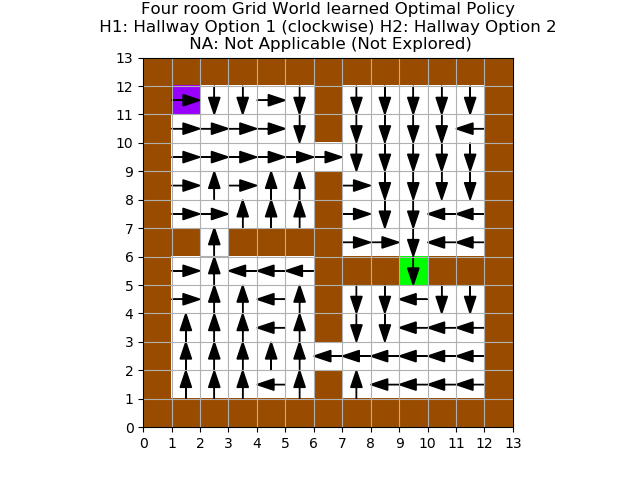
\includegraphics[width=0.43\linewidth]{./O1_10000_Arrows.png}\label{grid_a_arrow}}
	\subfigure[Grid world with goal G2]
	{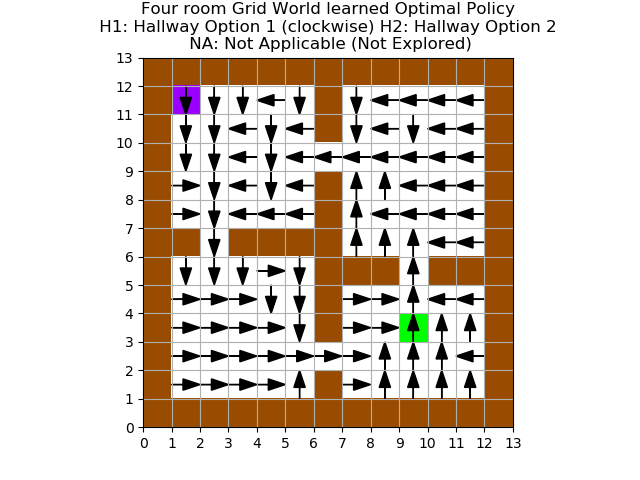
\includegraphics[width=0.43\linewidth]{./O2_10000_Arrows.png}\label{grid_b_arrow}}
	\caption{Grid world of four rooms.  Blue:Agent, Green:Terminal The grid world-\ref{grid_a_arrow} has terminal state G1 and grid world-\ref{grid_b_arrow} has terminal state G2. Arrow indicates the optimal policy. The policy in fig-\ref{grid_a_arrow} is obtained using option-1 where as same in fig.-\ref{grid_b_arrow} by option-2 }
	\label{fig:grids}
\end{figure}



To solve the defined problem, SMDP and Intra-option Q learning is utilized. The optimal policy is the fundamental thing for used methods. To obtain the optimal policy using Q-learning, the initial states were randomly selected and goal is directed to hallway. likewise, eight policy is obtained. The state values are obtained using the maximum return.

\begin{equation}
	V(s) = \argmax_{Q(s,a)} 
\end{equation}



\begin{figure}[H]
	\centering  
	\subfigure[State values with goal G1 by option-1]
	{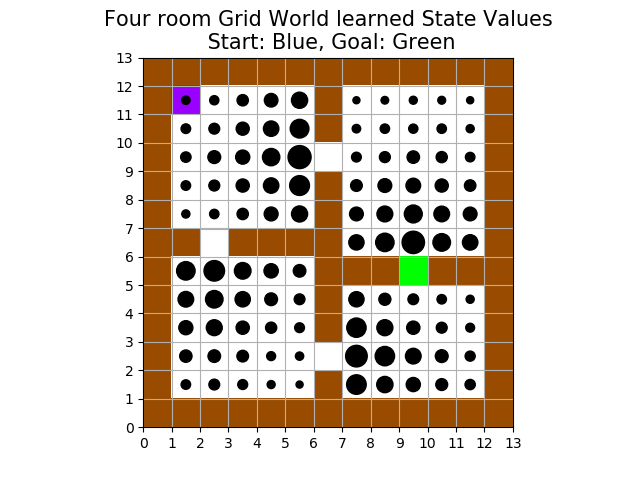
\includegraphics[width=0.43\linewidth]{./O1_10000_Circles.png}\label{grid_a_circle}}
	\subfigure[State values with goal G2 by option-2]
	{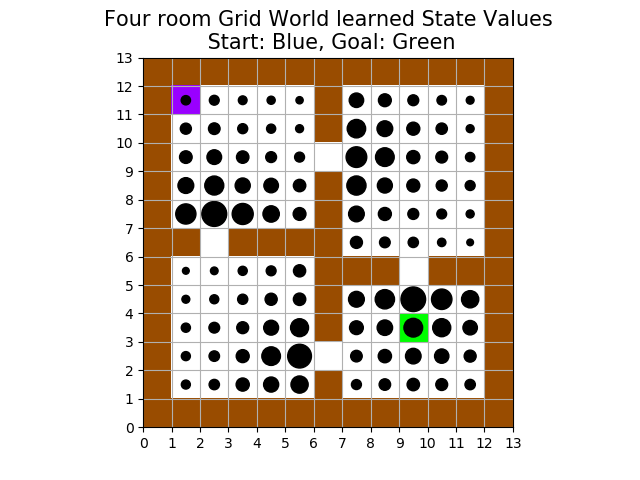
\includegraphics[width=0.43\linewidth]{./O2_10000_Circles.png}\label{grid_b_circle}}
	\caption{The grid world-\ref{grid_a_circle} has terminal state G1 and grid world-\ref{grid_b_circle} has terminal state G2. Circle size indicates the associated state value. The values in fig-\ref{grid_a_circle} is obtained using option-1 where as same in fig.-\ref{grid_b_circle} by option-2}
	\label{fig:state_val}
\end{figure}

The obtained optimal policy for goal-G1 and G2 is given in fig.-\ref{fig:grids}. The visualization of state values are given in fig.-\ref{fig:state_val}. For goal both goals, higher state values are obtained near hallways and terminal state. High state values are indicated by bigger size of circle.  \\

\textbf{SMDP Q-learning :}
\vspace{2mm}

Semi Markov Decision Processes are generalized MDPs, which allows policy maker to choose action according to change in state. It also provides the evolution of policy with continuous time while following arbitrary probability distribution. In short, SMDP follows the similar nature of MDP with options. Execution option starts with state $\mathcal{I}$ following policy $\pi$ and jumps to terminating state s'. The SMDP Q-learning updates for option-value function is given by,
\begin{equation}
	Q(s,o)  = Q(s,o) + \alpha [ r + \gamma^k \max_{o'\in s'} Q(s',o') - Q(s,o)]
\end{equation}
where, \\
k -  the number of time steps between s' and s \\
r - Cummulative discounted return over time\\
 
\textbf{Observation for Goal-G1:}

The learned optimal policy by SMDP-Q learning for goal-G1 is given in fig.-\ref{SMDP_G1_policy}. \textbf{The optimal policy is resultant of defined policy and primitive actions as well.} The primitive action are better than option away from goal and near the start state. Whereas, \textbf{near the terminal state Q-values are high and options play crucial role.}

Same can be observed from the state value diagram. \textbf{Near the goal state has higher valuer, which decrease as we move away from the goal.} Due to property of learning from experience and bound of wall near terminal state, in near the goal region there might be high chances of stumbling.  Some of the states are not explored as it possible to reach toward goal by following any option from those states. 

\begin{figure}[H]
	\centering  
	\subfigure[Optimal policy by SMDP-Q]
	{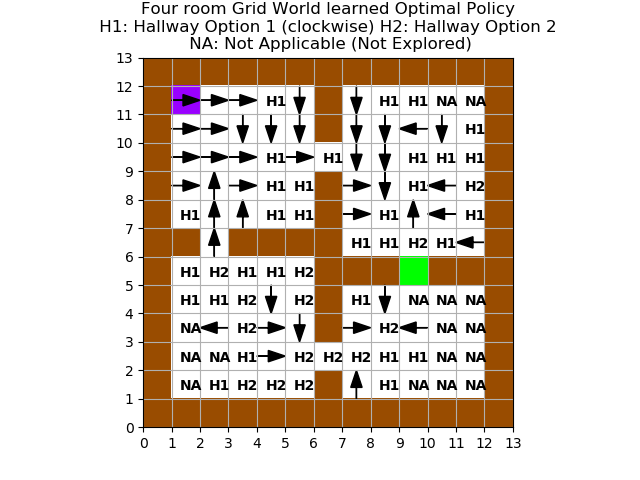
\includegraphics[width=0.45\linewidth]{./Q1_G1_10000_Arrows.png}\label{SMDP_G1_policy}}
	\subfigure[State values for SMDP-Q]
	{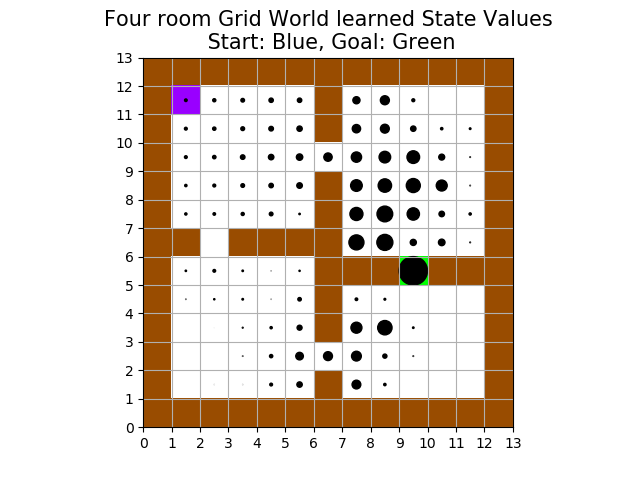
\includegraphics[width=0.45\linewidth]{./Q1_G1_10000_Circles.png}\label{SMDP_G1_value}}
	\caption{Grid world of four rooms.  Blue:Agent, Green:Terminal. The optimal policy-\ref{SMDP_G1_policy} and associated state values-\ref{SMDP_G1_value} for Goal-G1 after training of 10000 episodes.(By SMDP)}
	\label{fig:SMDP_G1}
\end{figure}

\newpage

\textbf{Observation for Goal-G2:}

The optimal policy for goal-G2 is given in fig.\ref{SMDP_G2_policy}. For this case also, states near the goal selects primitive action over policy as it helps agent to move away from the hallways and direct it towards goal whereas, states away from the goal follows actions. From figure-\ref{fig:SMDP_G2}, it is clear that SMDP Q-learning has obtained optimal policy using \textbf{mix of primitive action as well as options.}

\begin{figure}[H]
	\centering  
	\subfigure[Optimal policy by SMDP-Q]
	{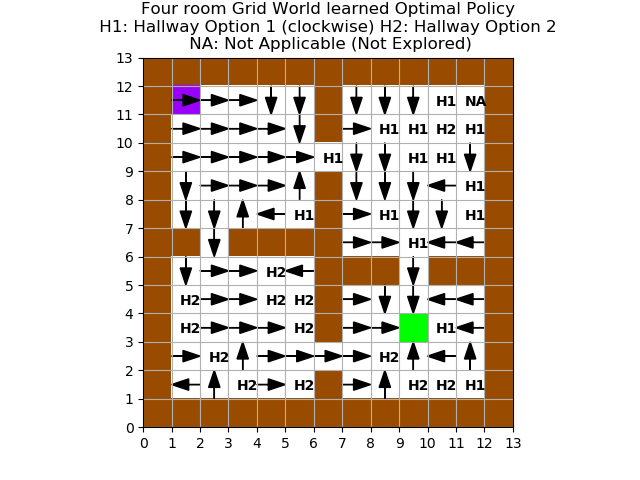
\includegraphics[width=0.45\linewidth]{./Q1_G2_10000_Arrows.png}\label{SMDP_G2_policy}}
	\subfigure[State values for SMDP-Q]
	{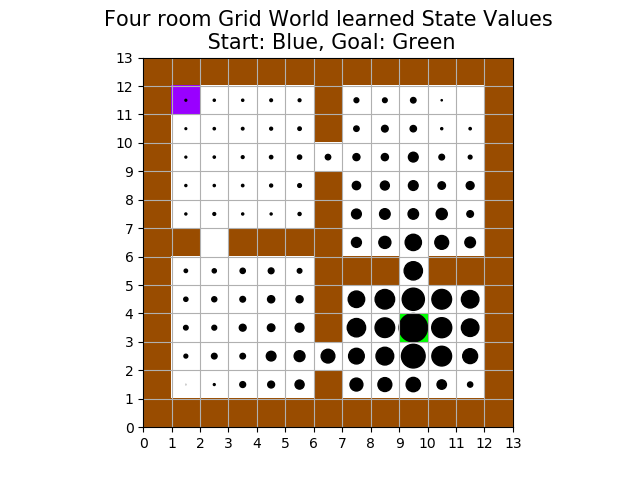
\includegraphics[width=0.45\linewidth]{./Q1_G2_10000_Circles.png}\label{SMDP_G2_value}}
	\caption{Grid world of four rooms.  Blue:Agent, Green:Terminal. The optimal policy-\ref{SMDP_G2_policy} and associated state values-\ref{SMDP_G2_value} for Goal-G2 after training of 10000 episodes.(By SMDP)}
	\label{fig:SMDP_G2}
\end{figure}
 For goal-2 compared to goal-1, the major states follow primitive actions where as options are dominant in case of goal-G1. Mainly for room-1 policy plays major role, whereas for room 2 and 4 it requires both.  \textbf{Near terminal state, dominance of policy make algorithm faster by increasing the learning rate.}

\newpage

\subsection{Answers-2 : Changed initial state to the centre of room 4}

\begin{figure}[H]
	\centering  
	\subfigure[Optimal policy for goal G1]
	{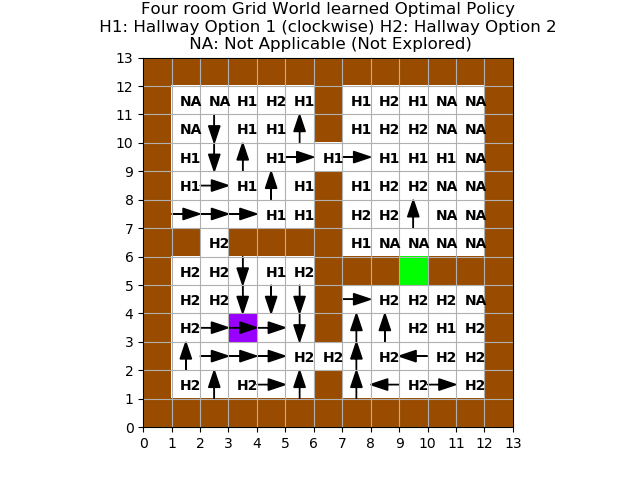
\includegraphics[width=0.45\linewidth]{./Q2_G1_10000_Arrows.png}\label{R4_SMDP_G1_policy}}
	\subfigure[State values for goal G1]
	{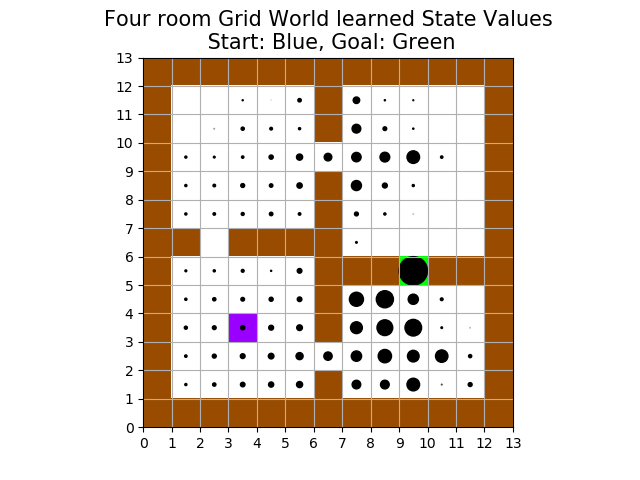
\includegraphics[width=0.45\linewidth]{./Q2_G1_10000_Circles.png}\label{R4_SMDP_G1_value}}
	\subfigure[Optimal policy for goal G2]
	{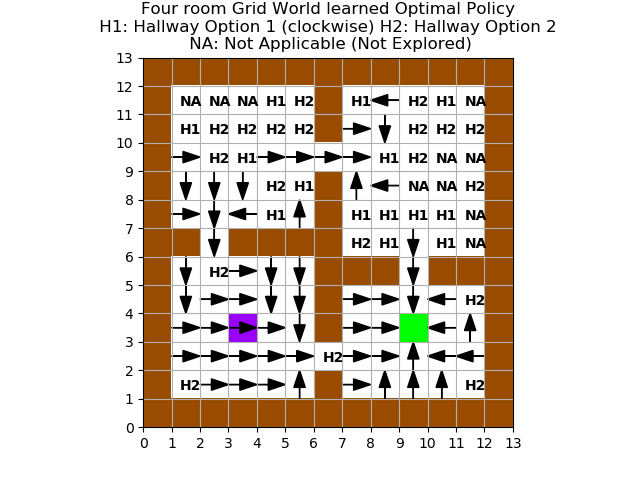
\includegraphics[width=0.45\linewidth]{./Q2_G2_10000_Arrows.png}\label{R4_SMDP_G2_policy}}
	\subfigure[State values for goal G2]
	{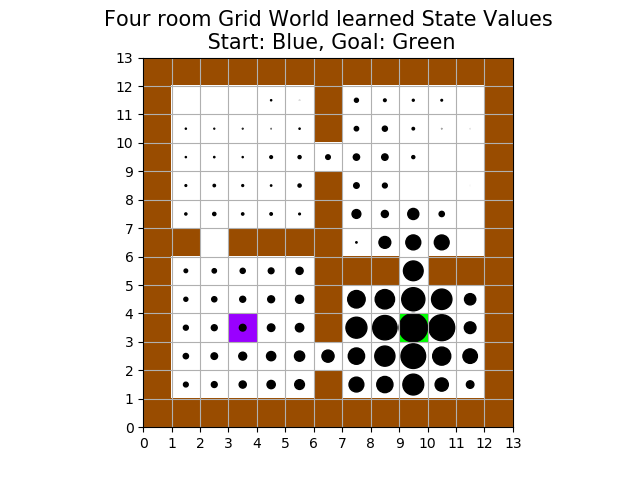
\includegraphics[width=0.45\linewidth]{./Q2_G2_10000_Circles.png}\label{R4_SMDP_G2_value}}
	\caption{Grid world of four rooms.  Blue:Agent, Green:Terminal. The optimal policy-\ref{R4_SMDP_G1_policy} and associated state values-\ref{R4_SMDP_G1_value} for Goal-G1 after training of 10000 episodes. Same way, the optimal policy-\ref{R4_SMDP_G2_policy} and associated state values-\ref{R4_SMDP_G2_value} for Goal-G2 (By SMDP) }
	\label{fig:R4_SMDP}
\end{figure}

\textbf{Observations:}

For the same terminal state, initial state is directed to center of room-4. \textbf{The change in state also causes the change in value function and optimal policy.} The optimal policy obtained in these cases are also mixtures of options as well as primitive actions. 

Change of state does not affect the role of primitive action and policy near the terminal states as well as far away from it. The major difference in both scenario (policy for same goal and change of initial state) is change in state value function. By comparing the fig.-\ref{SMDP_G1_policy} and fig.-\ref{R4_SMDP_G1_policy}, it is clear that the \textbf{state value of adjutant room of terminal and start state has higher state values. Change of the initial state directly affect the optimal policy, which varies in both scenario and finds the best possible route using primitive action and options.}

 The value obtained in case of goal G2 is higher and shows nature of gradient. As goal-G1 is constrained by two wall these varies in this case. Options play vital role near terminal state of goal-G1, whereas, primitive actions play important role in case of goal-G2.
 
 \newpage

\subsection{Bonus Answers-3: Intra-option Q learning} 

Intra option Q learning learns from the execution of one policy while it following another behavioral policy. It is an off policy algorithm. The downside about SMDP is that it has to execute a termination condition and due to that only single option is applied at time. This limitation is removed in Intra-option Q learning. It can learn different options at time without prior execution of option from same experience. The update rule for intra-option Q learning is given in as below,
\begin{equation}
\begin{aligned}
Q(s,0) &= Q(s,o) + \alpha(s,0) [r+\gamma \hat{Q}(s',o) - Q(s,o)] \\
\hat{Q}(s,0) &= (1-\beta(s')) Q(s',o) + \beta(s')  \max_{o'\in s'} Q(s',o')
\end{aligned}
\end{equation}
\textbf{For Intial State in Upper Left Corner:} 
\begin{figure}[H]
	\centering  
	\subfigure[Optimal policy for goal G1]
	{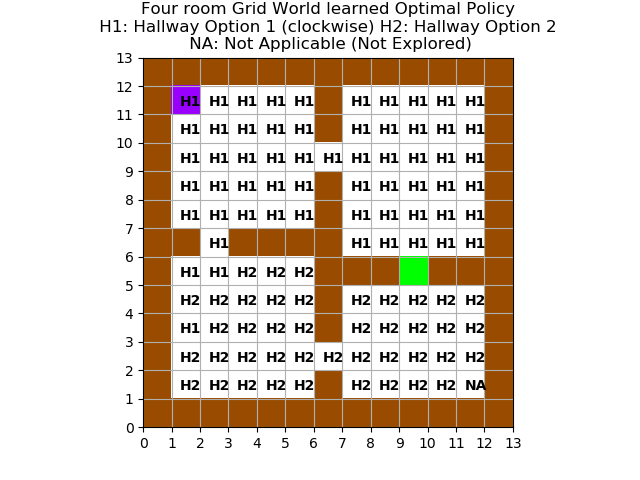
\includegraphics[width=0.45\linewidth]{./Q3_G1_10000_Arrows.png}\label{R1_Intra_G1_policy}}
	\subfigure[State values for goal G1]
	{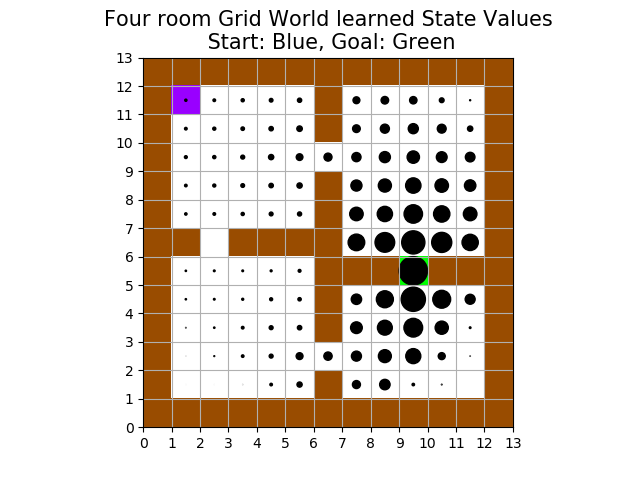
\includegraphics[width=0.45\linewidth]{./Q3_G1_10000_Circles.png}\label{R1_Intra_G1_value}}
	\subfigure[Optimal policy for goal G2]
	{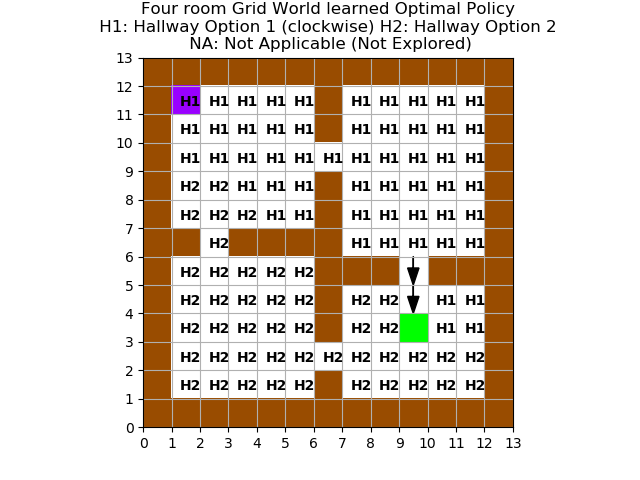
\includegraphics[width=0.45\linewidth]{./Q3_G2_10000_Arrows.png}\label{R1_Intra_G2_policy}}
	\subfigure[State values for goal G2]
	{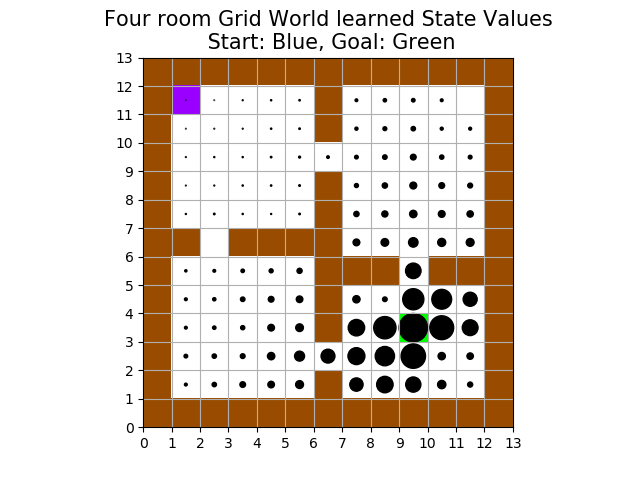
\includegraphics[width=0.45\linewidth]{./Q3_G2_10000_Circles.png}\label{R1_Intra_G2_value}}
	\caption{Grid world of four rooms.  Blue:Agent, Green:Terminal. The optimal policy-\ref{R1_Intra_G1_policy} and associated state values-\ref{R1_Intra_G1_value} for Goal-G1 after training of 10000 episodes. Same way, the optimal policy-\ref{R1_Intra_G2_policy} and associated state values-\ref{R1_Intra_G2_value} for Goal-G2 (By Intra option Q learning)}
	\label{fig:R1_Intra}
\end{figure}

\textbf{Observation and Improvement:}


The intra-option Q learning, learns most possible option. It can be observed that, it \textbf{only uses correct options to reach the goal.} The optimal policy does not change by learning from more episodes. By comparing result of SMDP and intra-option, it is clear that for 10000 episodes intra-option Q learning outperforms the SMDP. Even around \textbf{1000 episodes are enough to give similar result in case of intra-opion Q learning. }

From figure-\ref{fig:R1_Intra}, it can be seen that for \textbf{goal-G1 optimal policy is learned only using correct options rather than primitive actions.} For goal-G2, \textbf{it is not using any primitive action till goal-G1 as the agent has learned to reach the goal. After that, it just take primitive action from near goal location.} \\


\textbf{For Initial State in the center of room-4 :} \\

 Similar observation has been made by transferring the initial state to center of the room-4 as given in fig.-\ref{fig:R4_Intra}. \textbf{For goal-G1 it has only obtained the optimal policy using options. Once it has learned to reach that state then change of goal is attained by primitive actions.} \\
 

\begin{figure}[H]
	\centering  
	\subfigure[Optimal policy for goal G1]
	{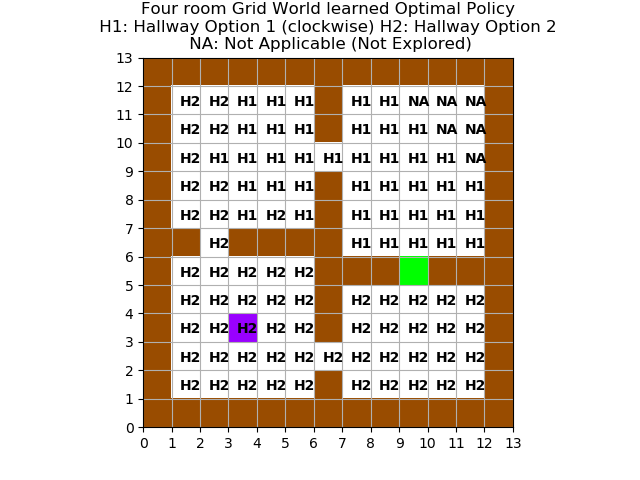
\includegraphics[width=0.45\linewidth]{./Q4_G1_10000_Arrows.png}\label{R4_Intra_G1_policy}}
	\subfigure[State values for goal G1]
	{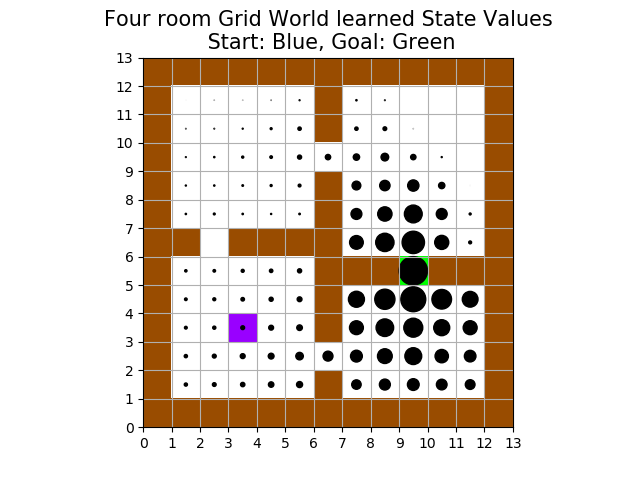
\includegraphics[width=0.45\linewidth]{./Q4_G1_10000_Circles.png}\label{R4_Intra_G1_value}}
	\subfigure[Optimal policy for goal G2]
	{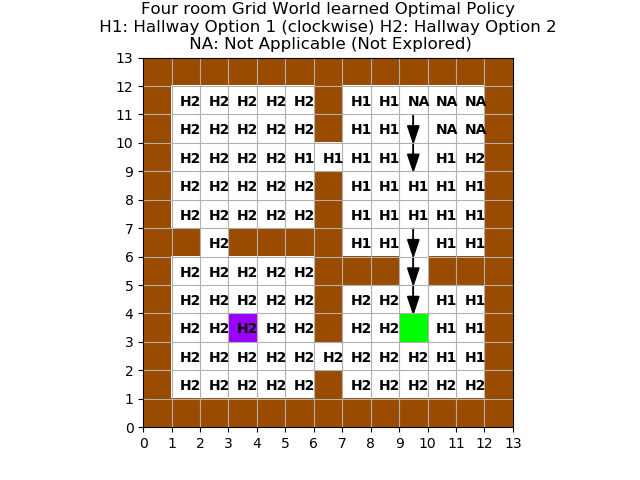
\includegraphics[width=0.45\linewidth]{./Q4_G2_10000_Arrows.png}\label{R4_Intra_G2_policy}}
	\subfigure[State values for goal G2]
	{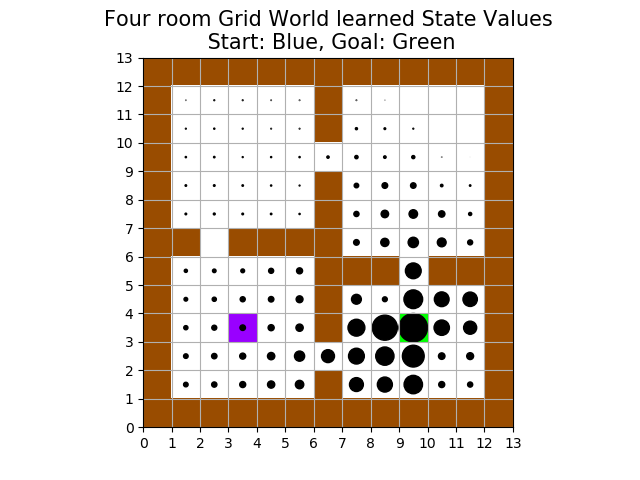
\includegraphics[width=0.45\linewidth]{./Q4_G2_10000_Circles.png}\label{R4_Intra_G2_value}}
	\caption{Grid world of four rooms.  Blue:Agent, Green:Terminal. The optimal policy-\ref{R4_Intra_G1_policy} and associated state values-\ref{R4_Intra_G1_value} for Goal-G1 after training of 10000 episodes. Same way, the optimal policy-\ref{R4_Intra_G2_policy} and associated state values-\ref{R4_Intra_G2_value} for Goal-G2  (By Intra option Q learning)}
	\label{fig:R4_Intra}
\end{figure}


 \subsection{Learning Curves of Average Return and Steps :}
  For all the possible cases comparative graphs of average return and average steps is mentioned here. 
 
 \begin{figure}[H]
 	\centering  
 	\subfigure[Number of average steps for goal G1]
 	{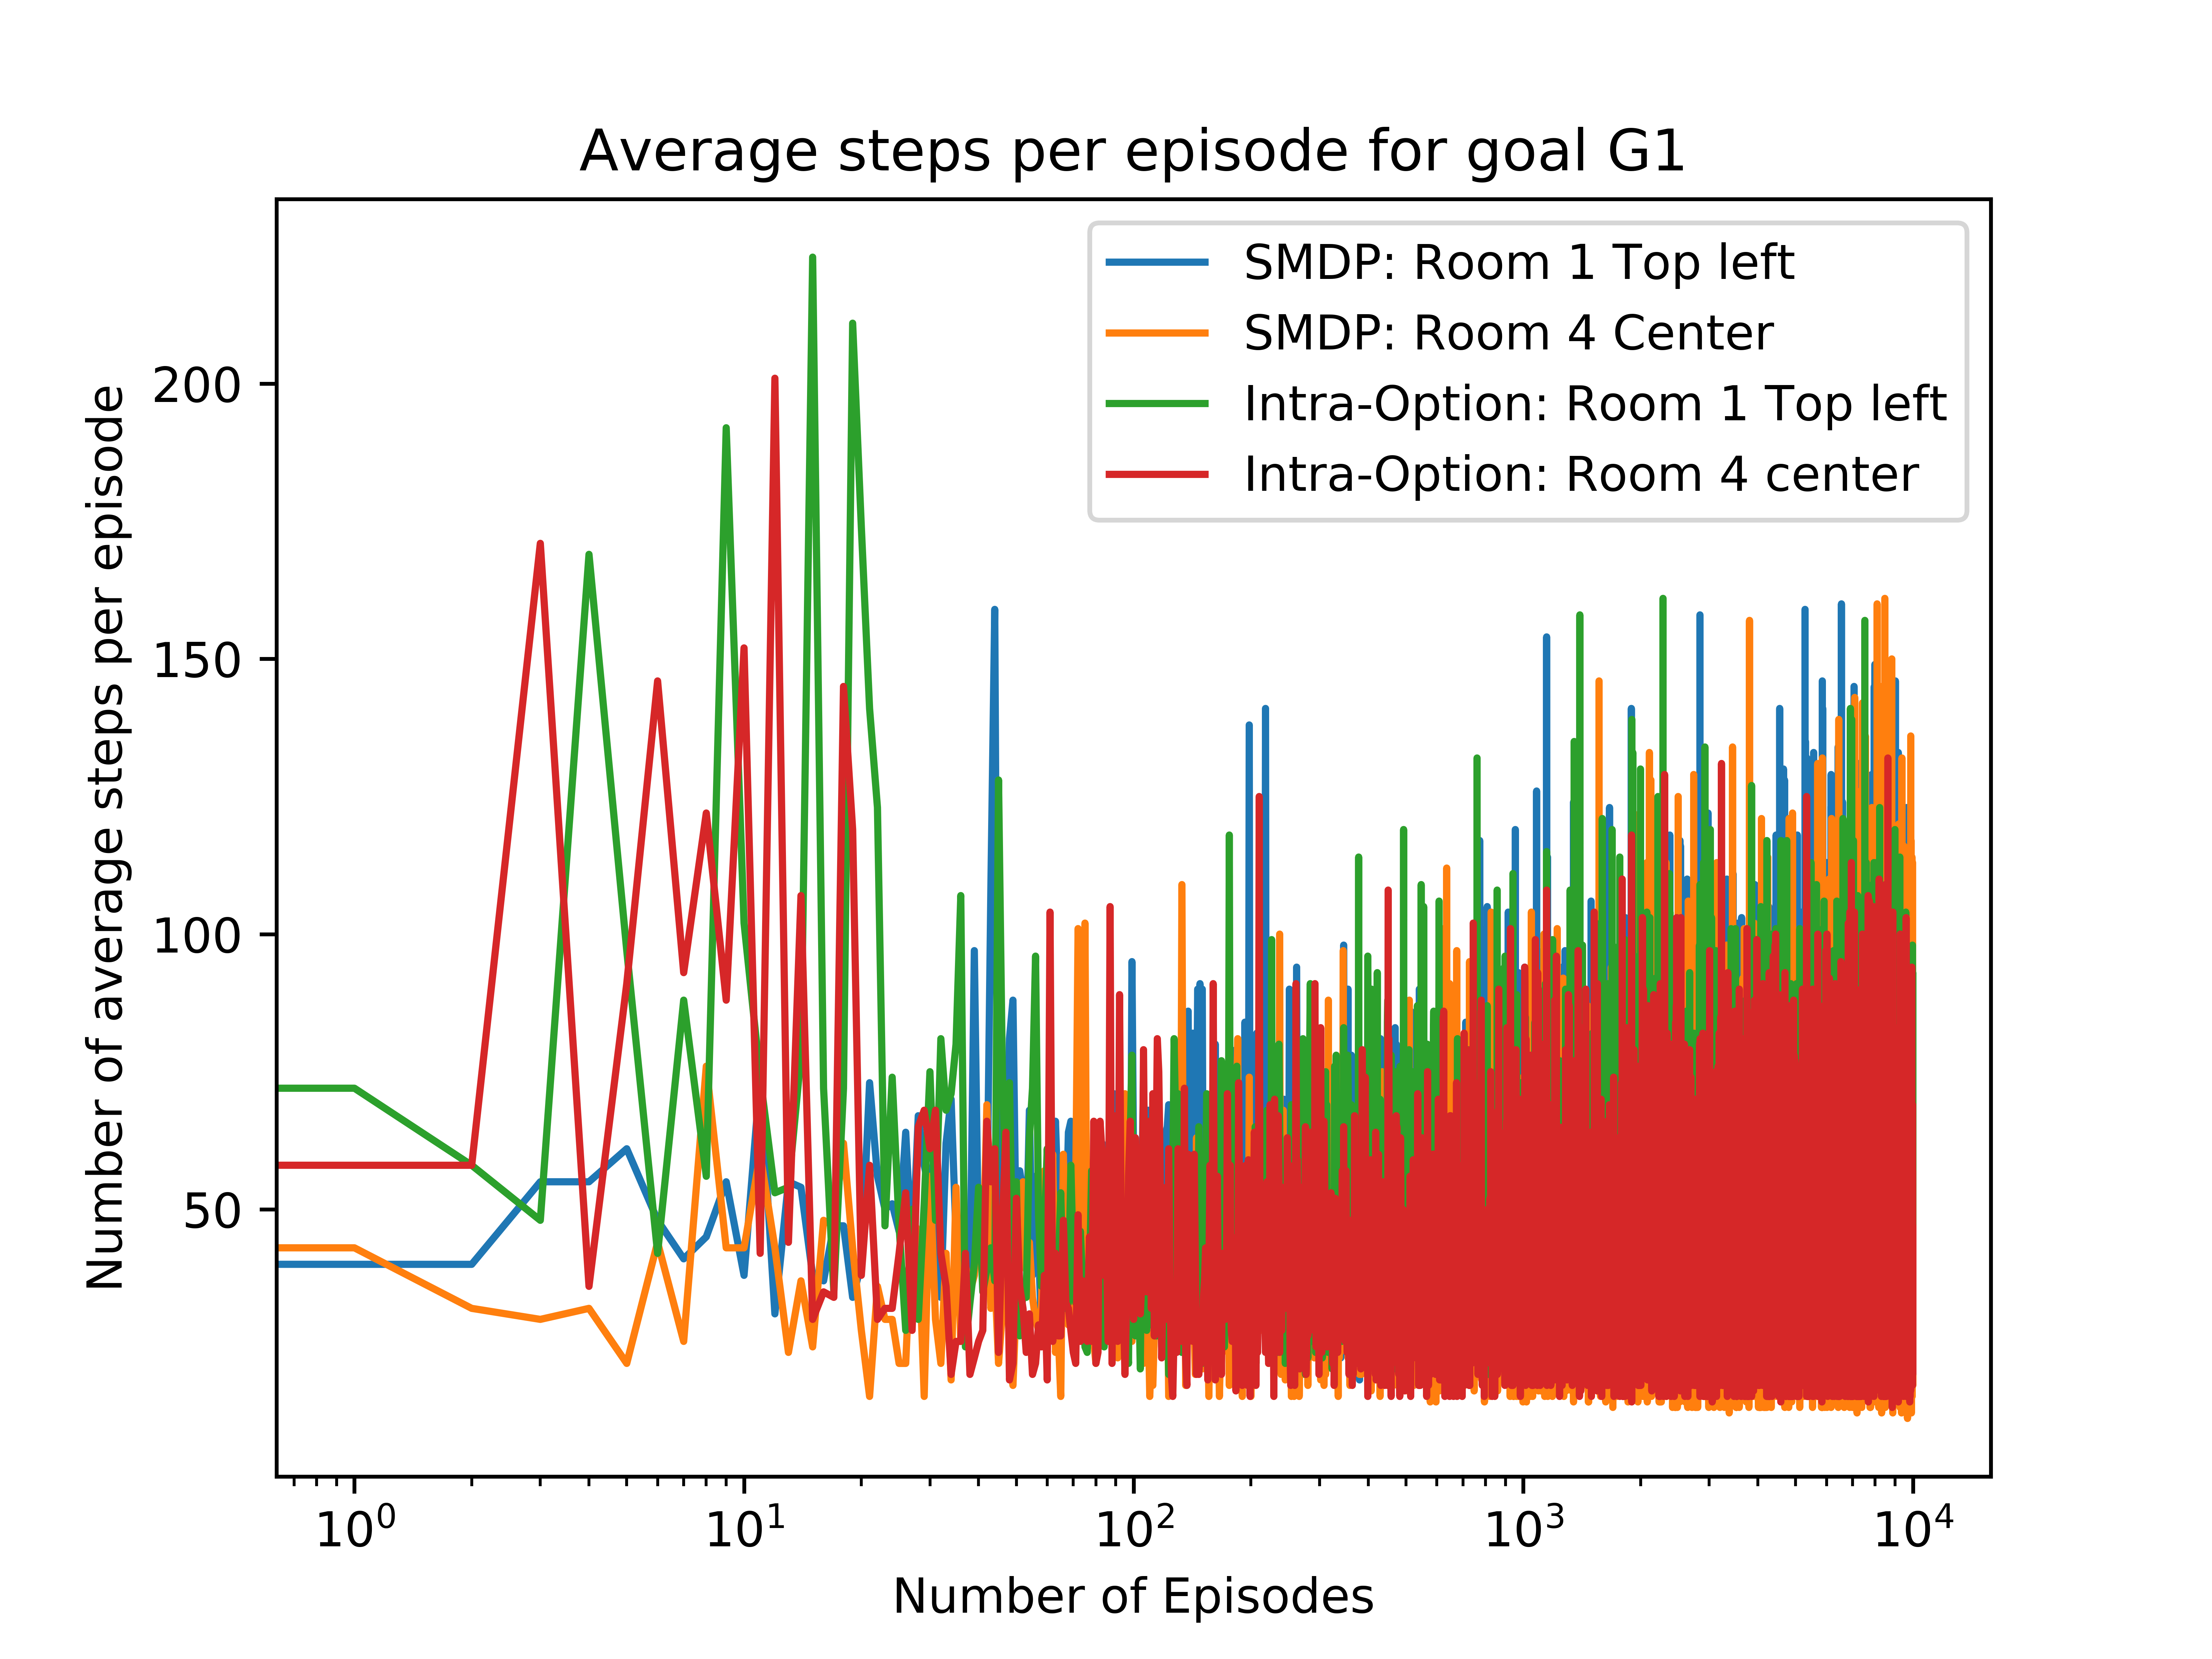
\includegraphics[width=0.4\linewidth]{./Avg_steps_G1.png}\label{avg_steps_G1}}
 	\subfigure[Number of average steps for goal G2]
 	{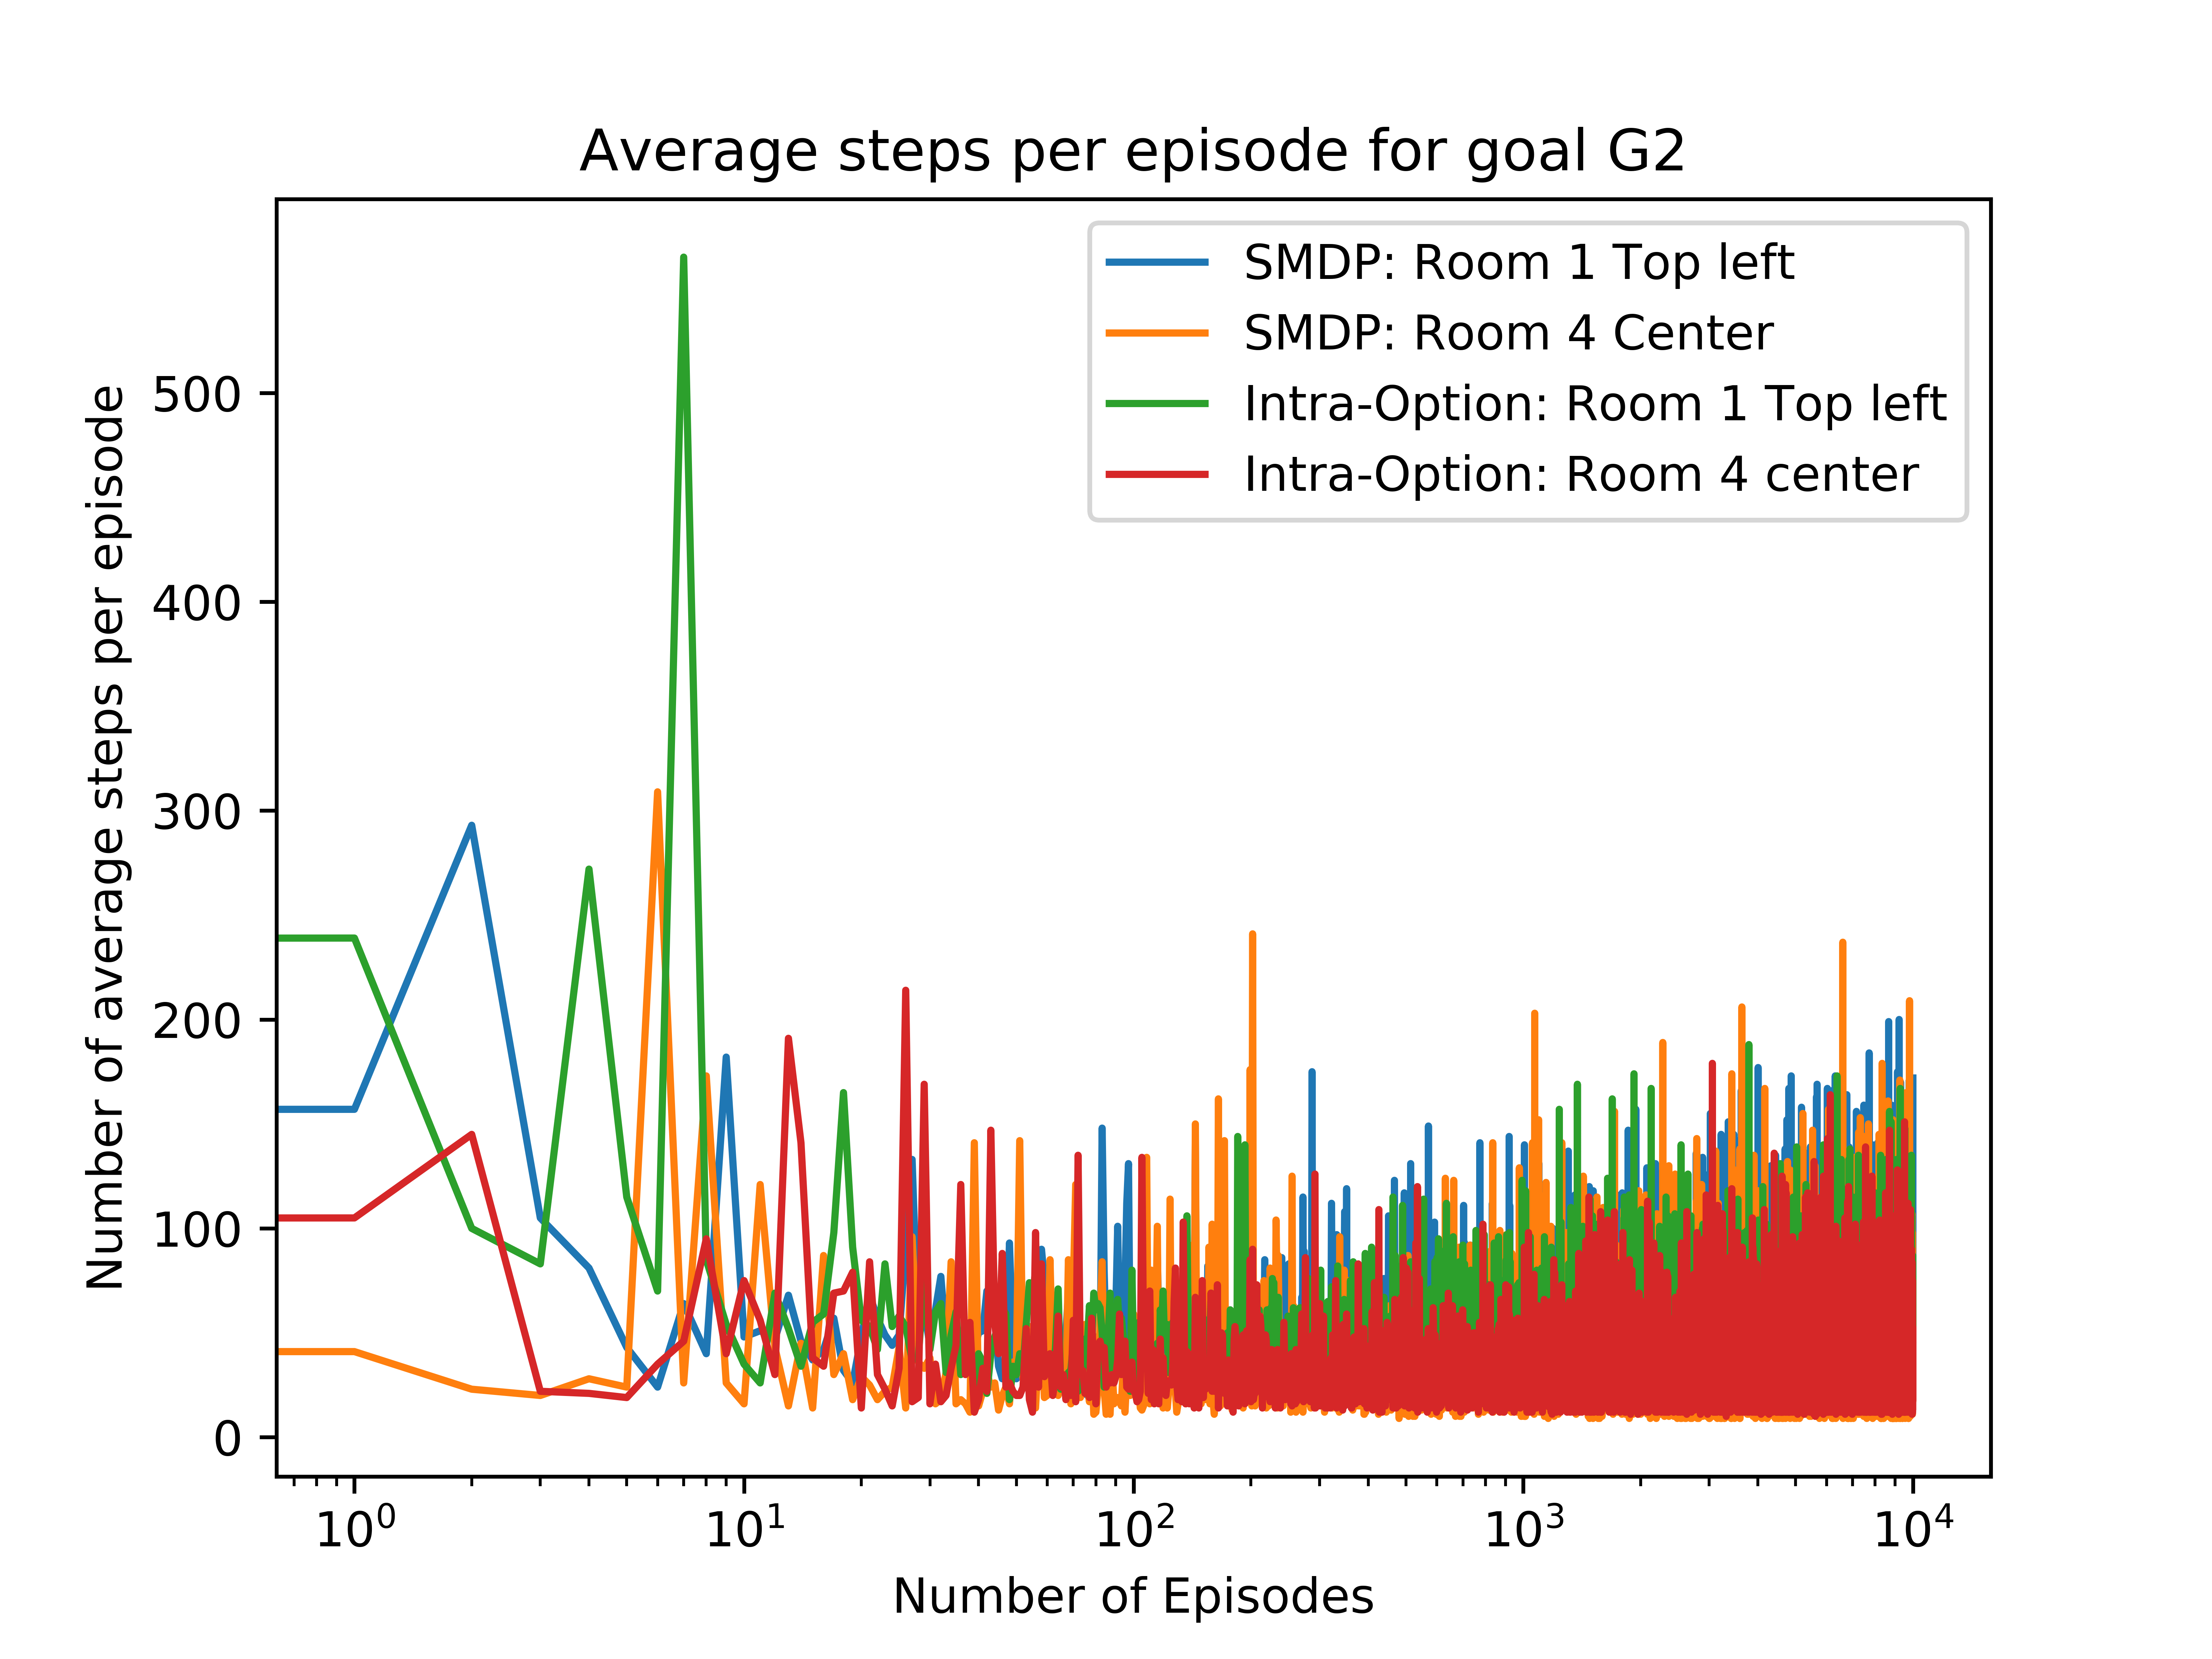
\includegraphics[width=0.4\linewidth]{./Avg_steps_G2.png}\label{avg_steps_G2}}
 	\caption{Total number of average steps in case of initiation of agent at different states for SMDP and Intra-Option Q learning for goal-G1 \ref{avg_steps_G1} and for goal-G2-\ref{avg_steps_G2}}
 	\label{fig:Avg_stes}
 \end{figure}
 
 As given in fig.-\ref{avg_steps_G1} in case for goal G1 for SMDP, initially as it does the exploration and takes more steps to reach the goal. SMDP takes on average 50 steps per episode which goes to 75 steps and almost remains constant. Whereas,\textbf{ when initial state is shifted to center of the room-4, the number of average steps taken are slightly lesser in case of SMDP.}
 
 Intra option Q learning has tendency to learn from applicable options of past experience so \textbf{initially due to exploration, intra option takes slightly more steps then SMDP.}  But once it has learned the policy, l\textbf{ater the average steps comes down significantly.  Further requires around half amount of average steps in learning the policy. } 
 
 Similar observation can be made for goal-G2. \textbf{Initially average steps taken by intra-option method is almost double but with increase in number of episodes intra option learns faster and outperforms the SMDP.} 
 
  
 \begin{figure}[H]
 	\centering  
 	\subfigure[Total return vs epsiode for goal G1]
 	{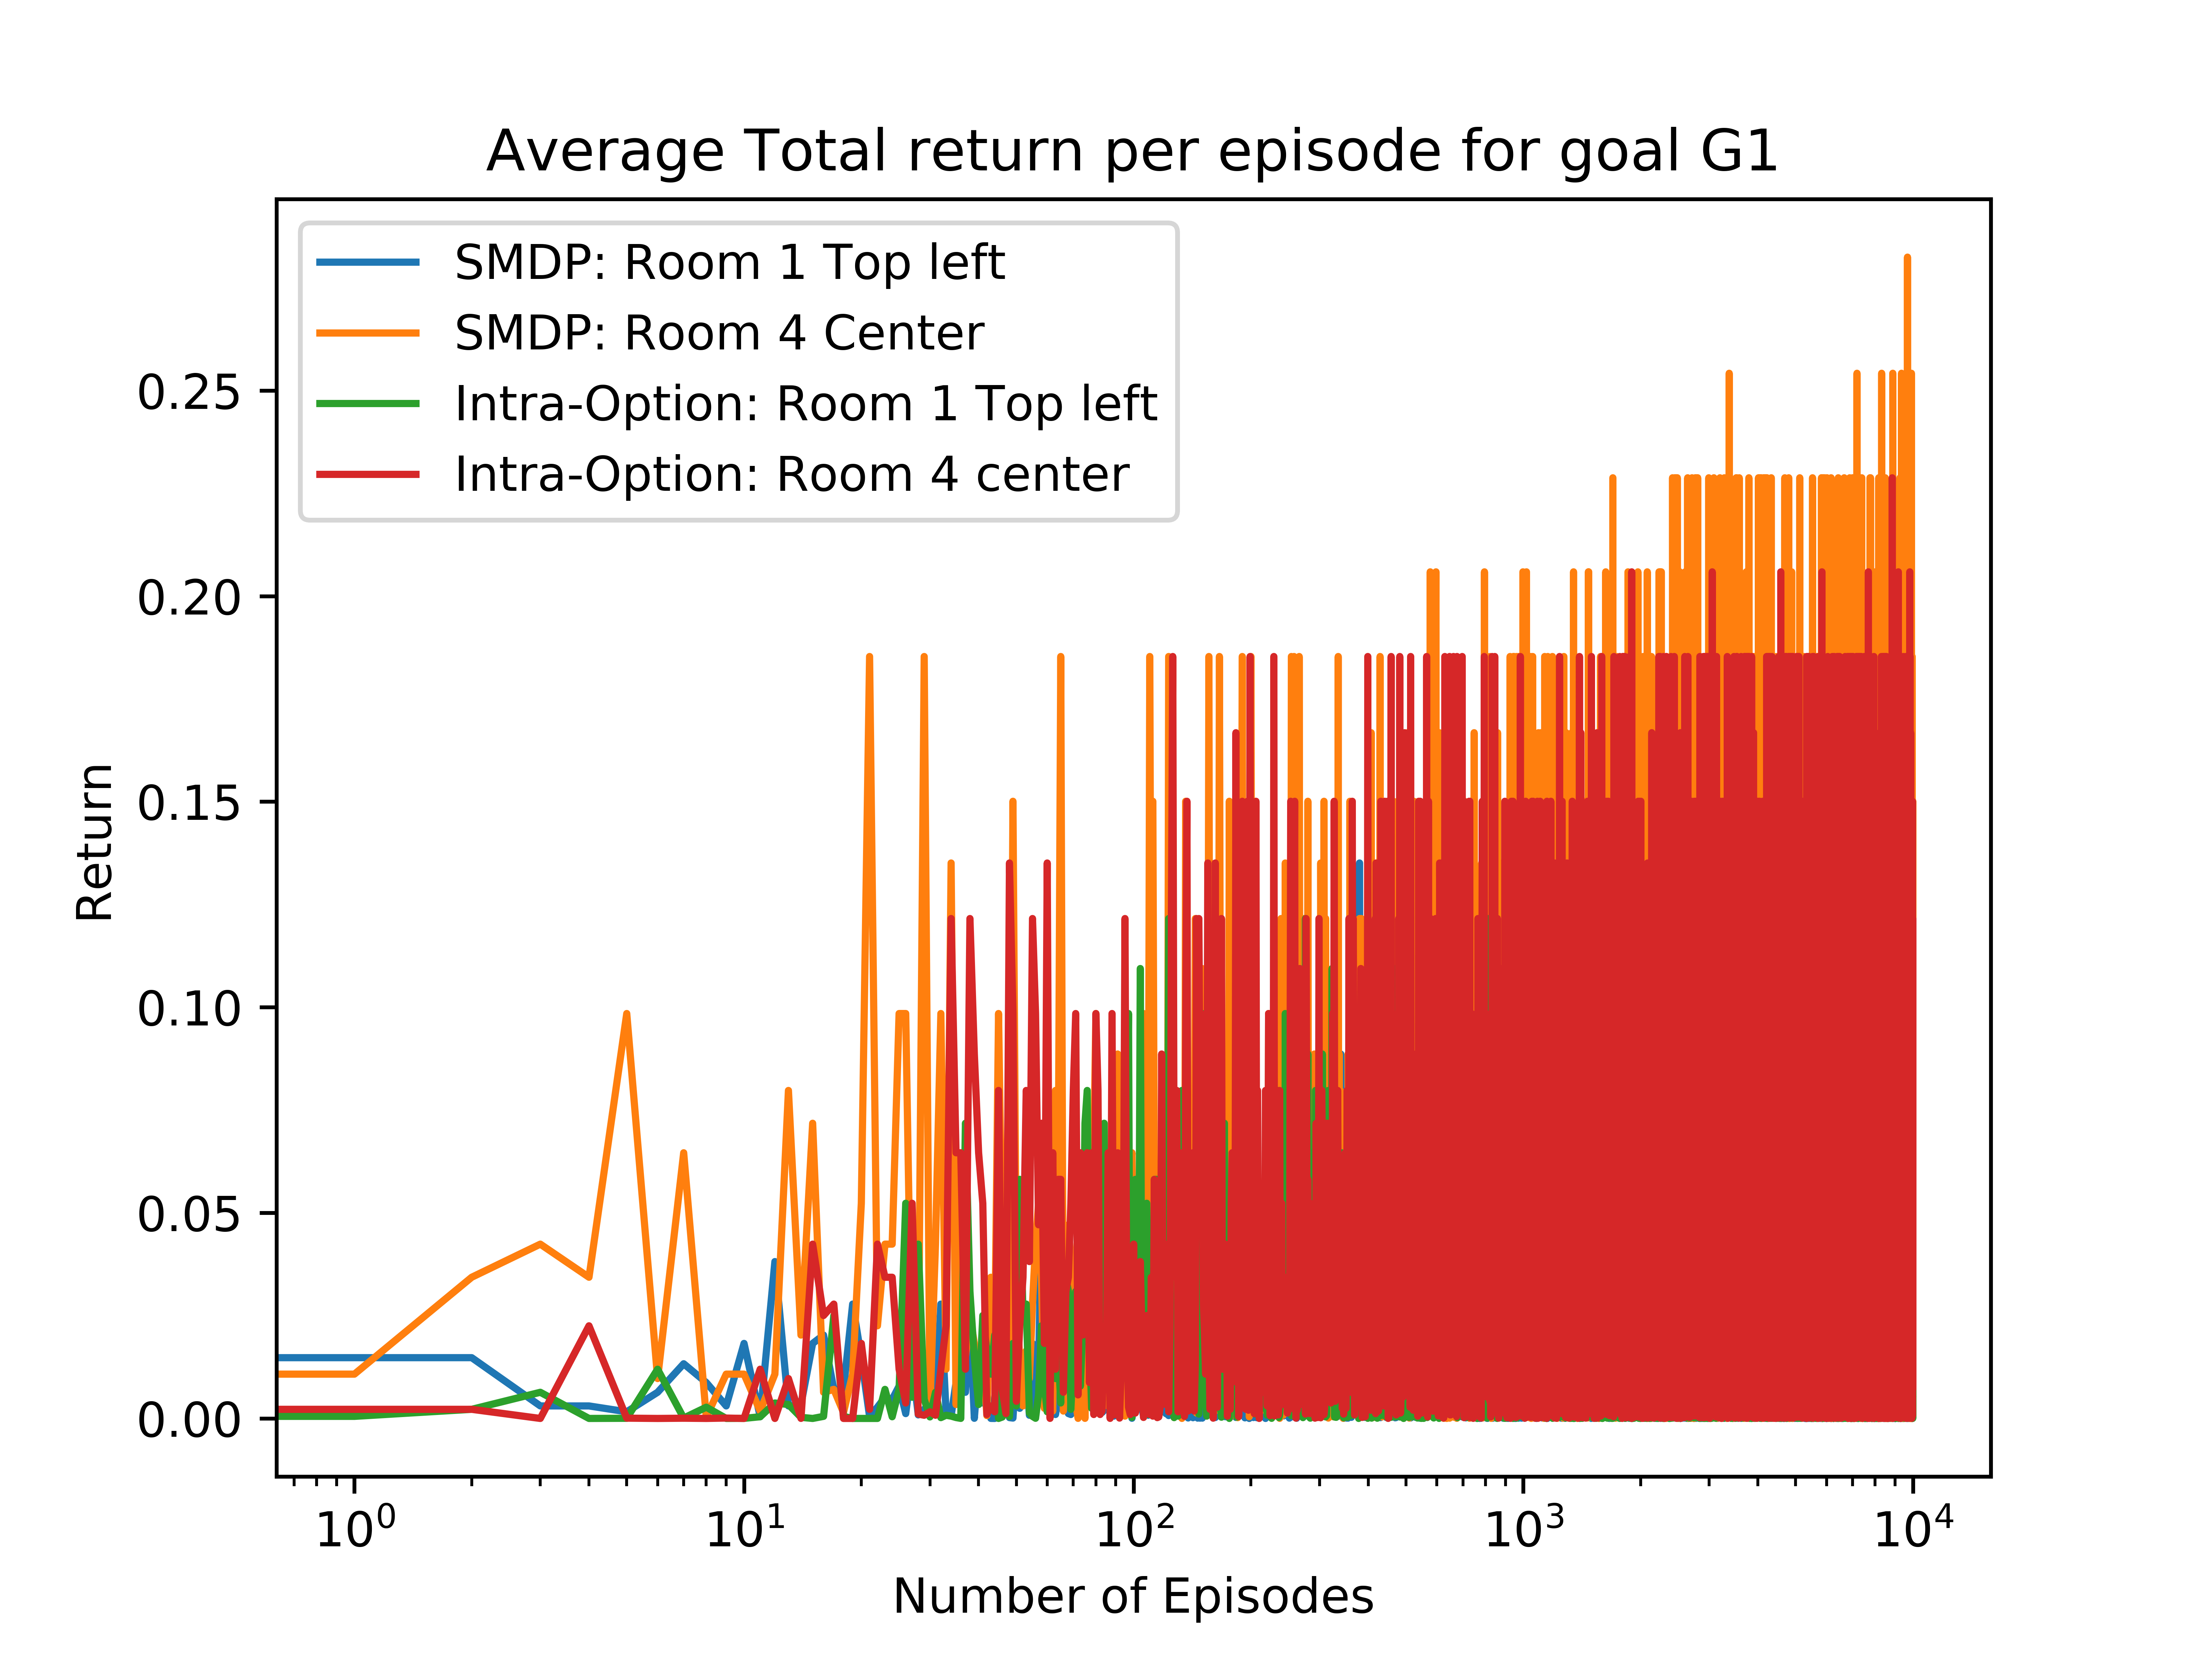
\includegraphics[width=0.4\linewidth]{./Total_return_steps_G1.png}\label{action_G1}}
 	\subfigure[Total return vs epsiode for goal G2]
 	{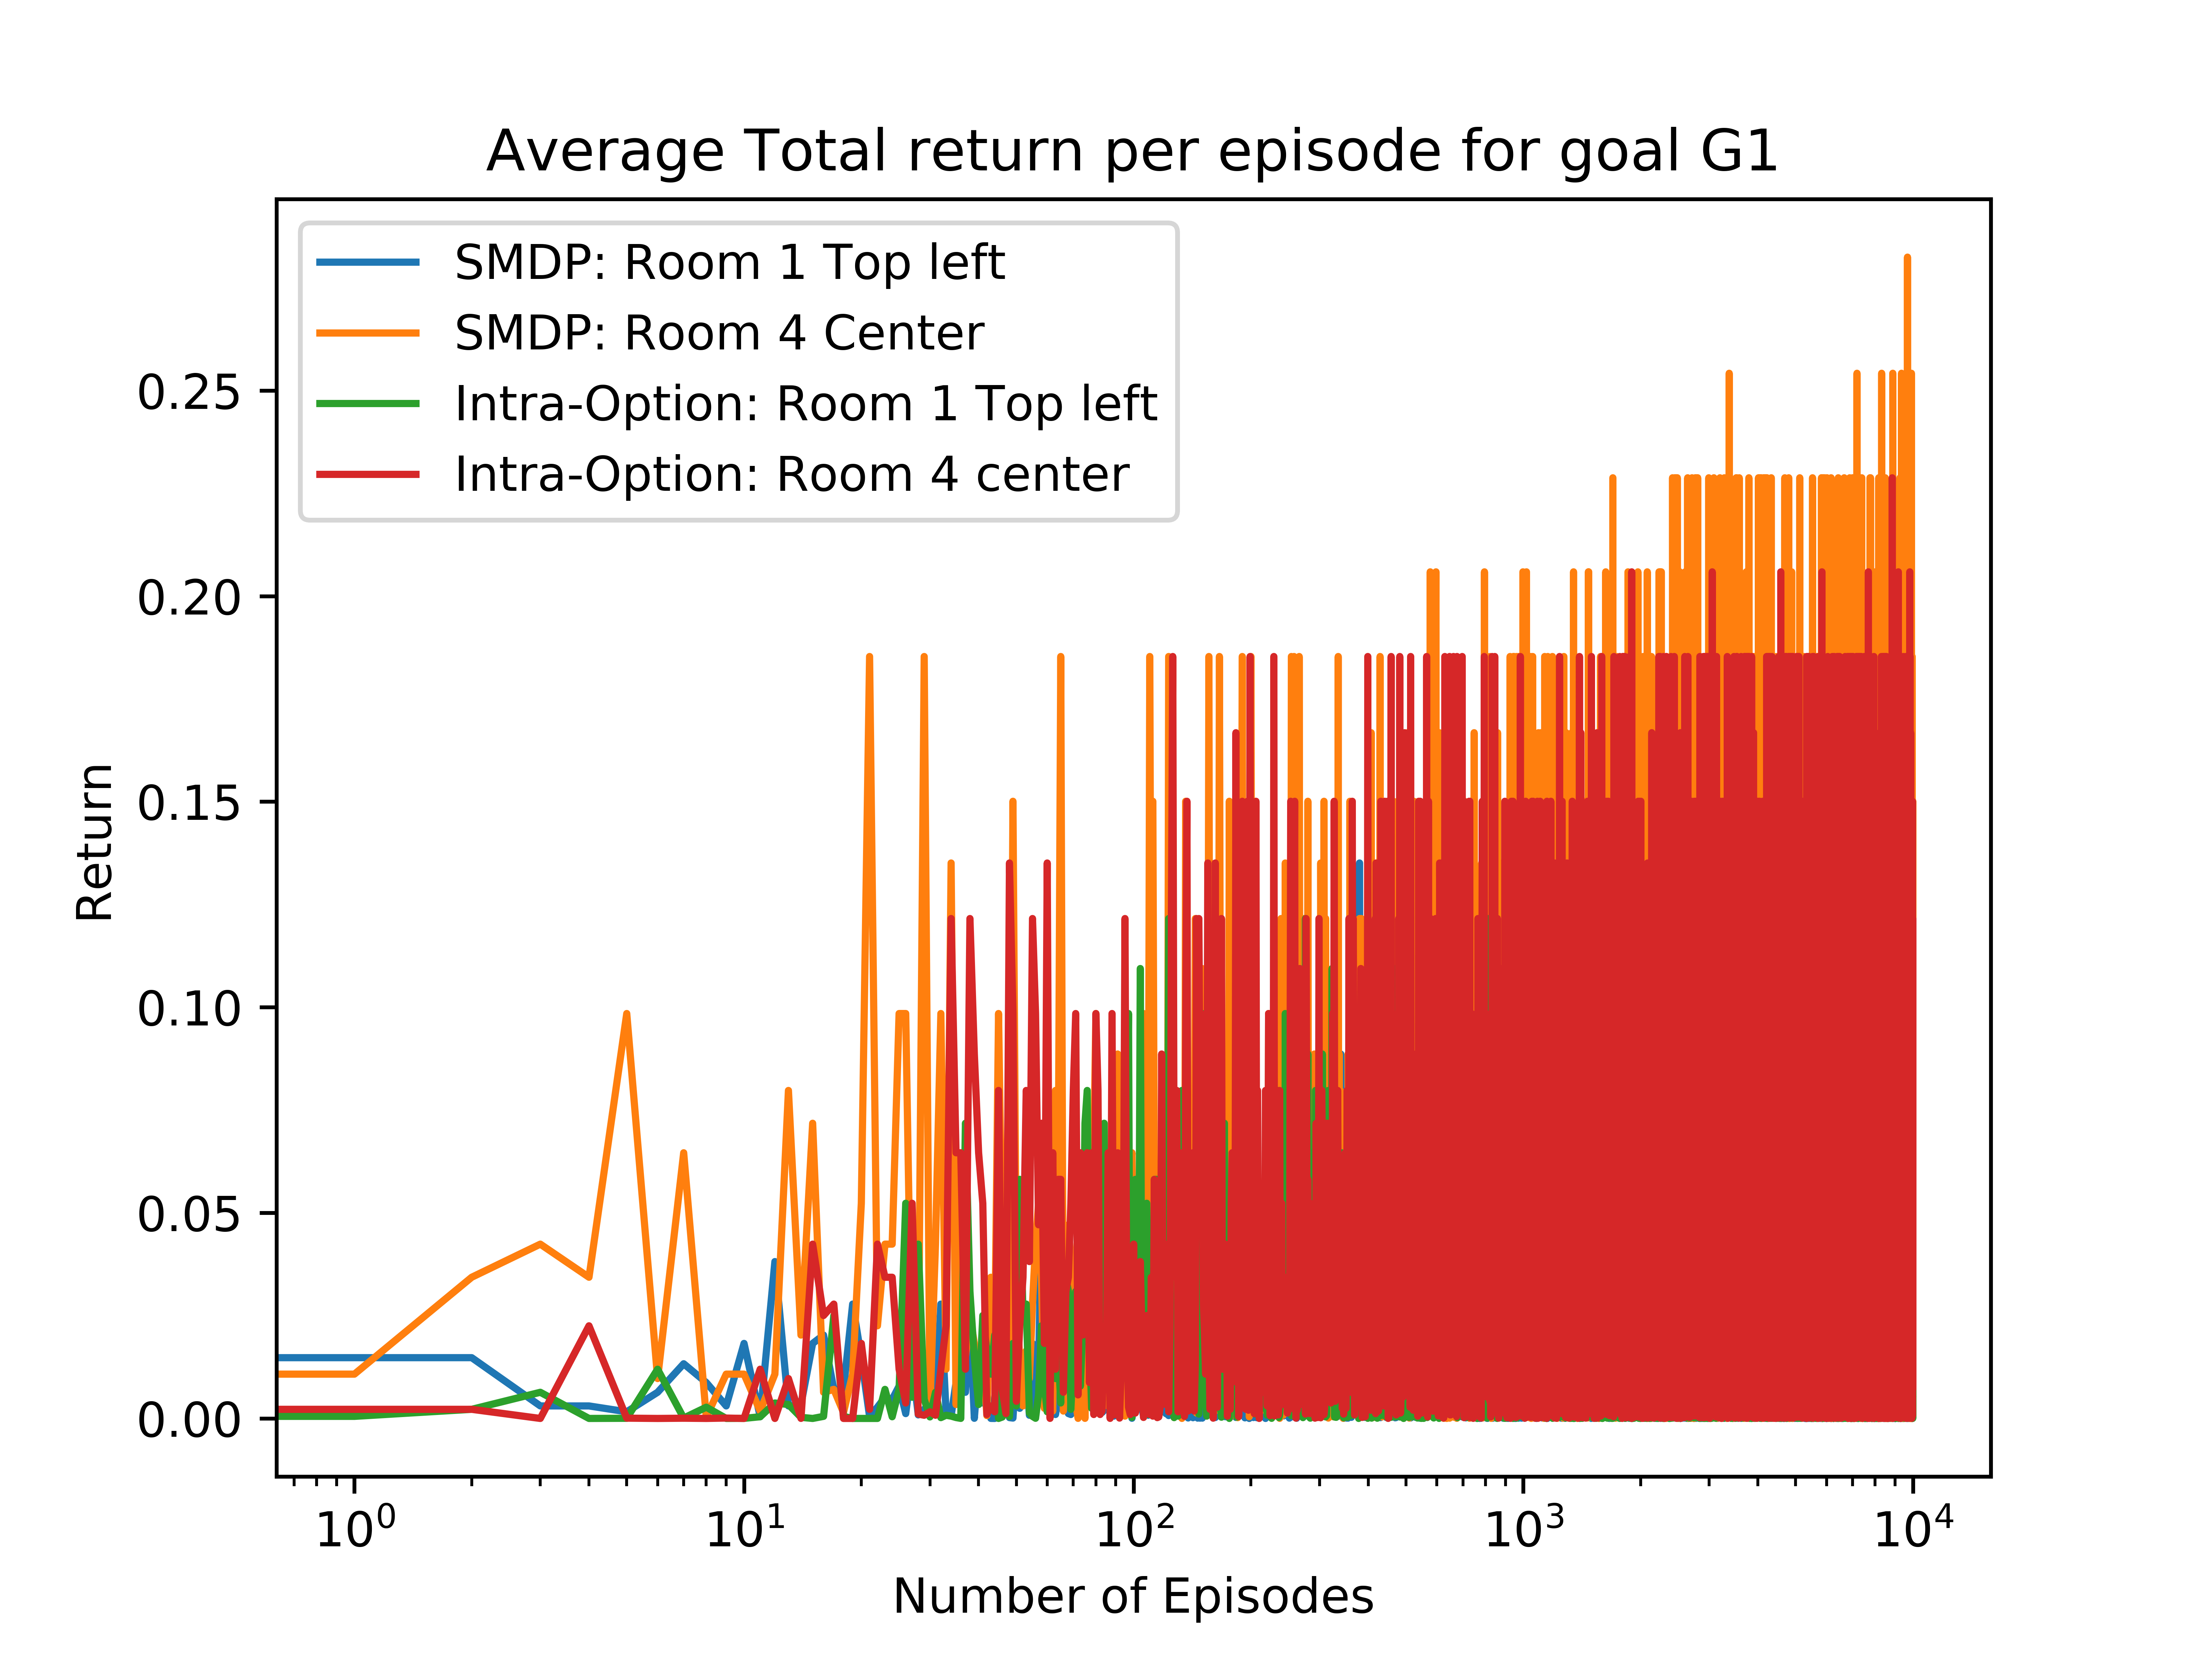
\includegraphics[width=0.4\linewidth]{./Total_return_steps_G1.png}\label{action_G2}}
 	\caption{Average total return by SMDP and Intra-option Q learning for goal-G1 \ref{avg_steps_G1} and for goal-G2-\ref{avg_steps_G2}. Each primitive action denotes the single step. The average is taken over 10 episodes and x-axis follows $\log 10$ scale.}
 	\label{fig:action}
 \end{figure}
 
  \begin{figure}[H]
  	\centering  
  	\subfigure[Total return vs epsiode for goal G1]
  	{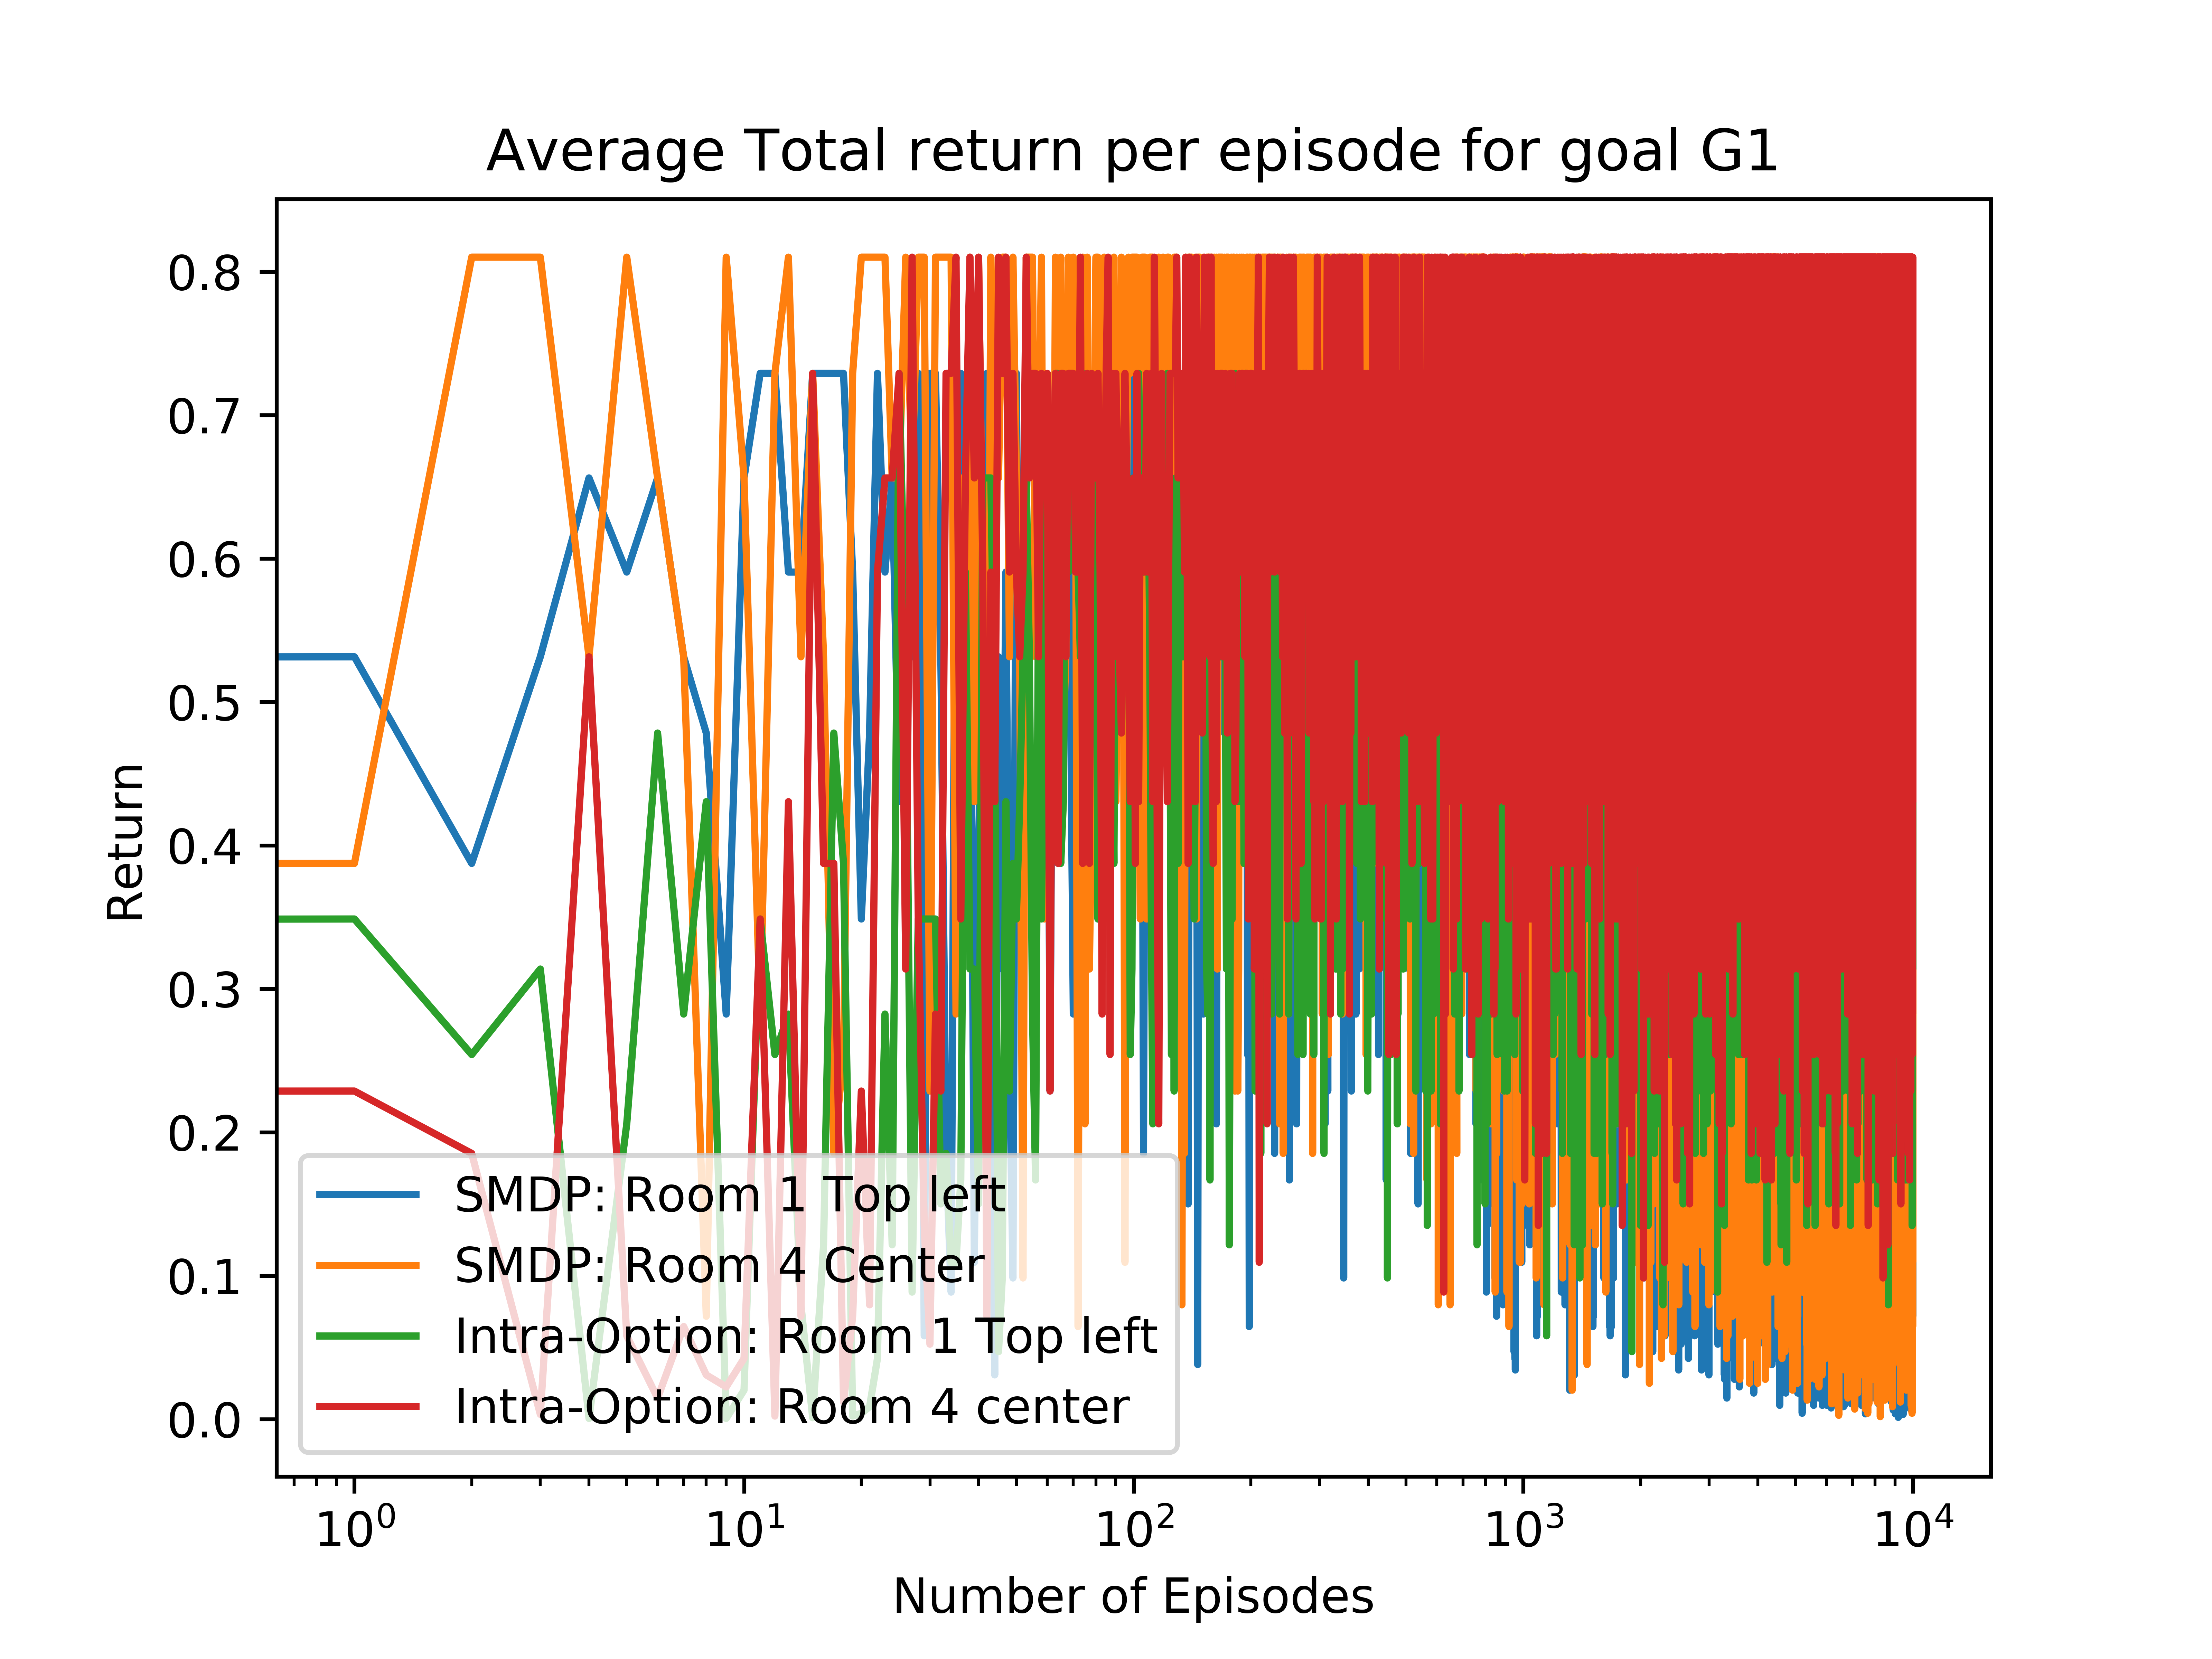
\includegraphics[width=0.4\linewidth]{./Total_return_G1.png}\label{option_G1}}
  	\subfigure[Total return vs epsiode for goal G2]
  	{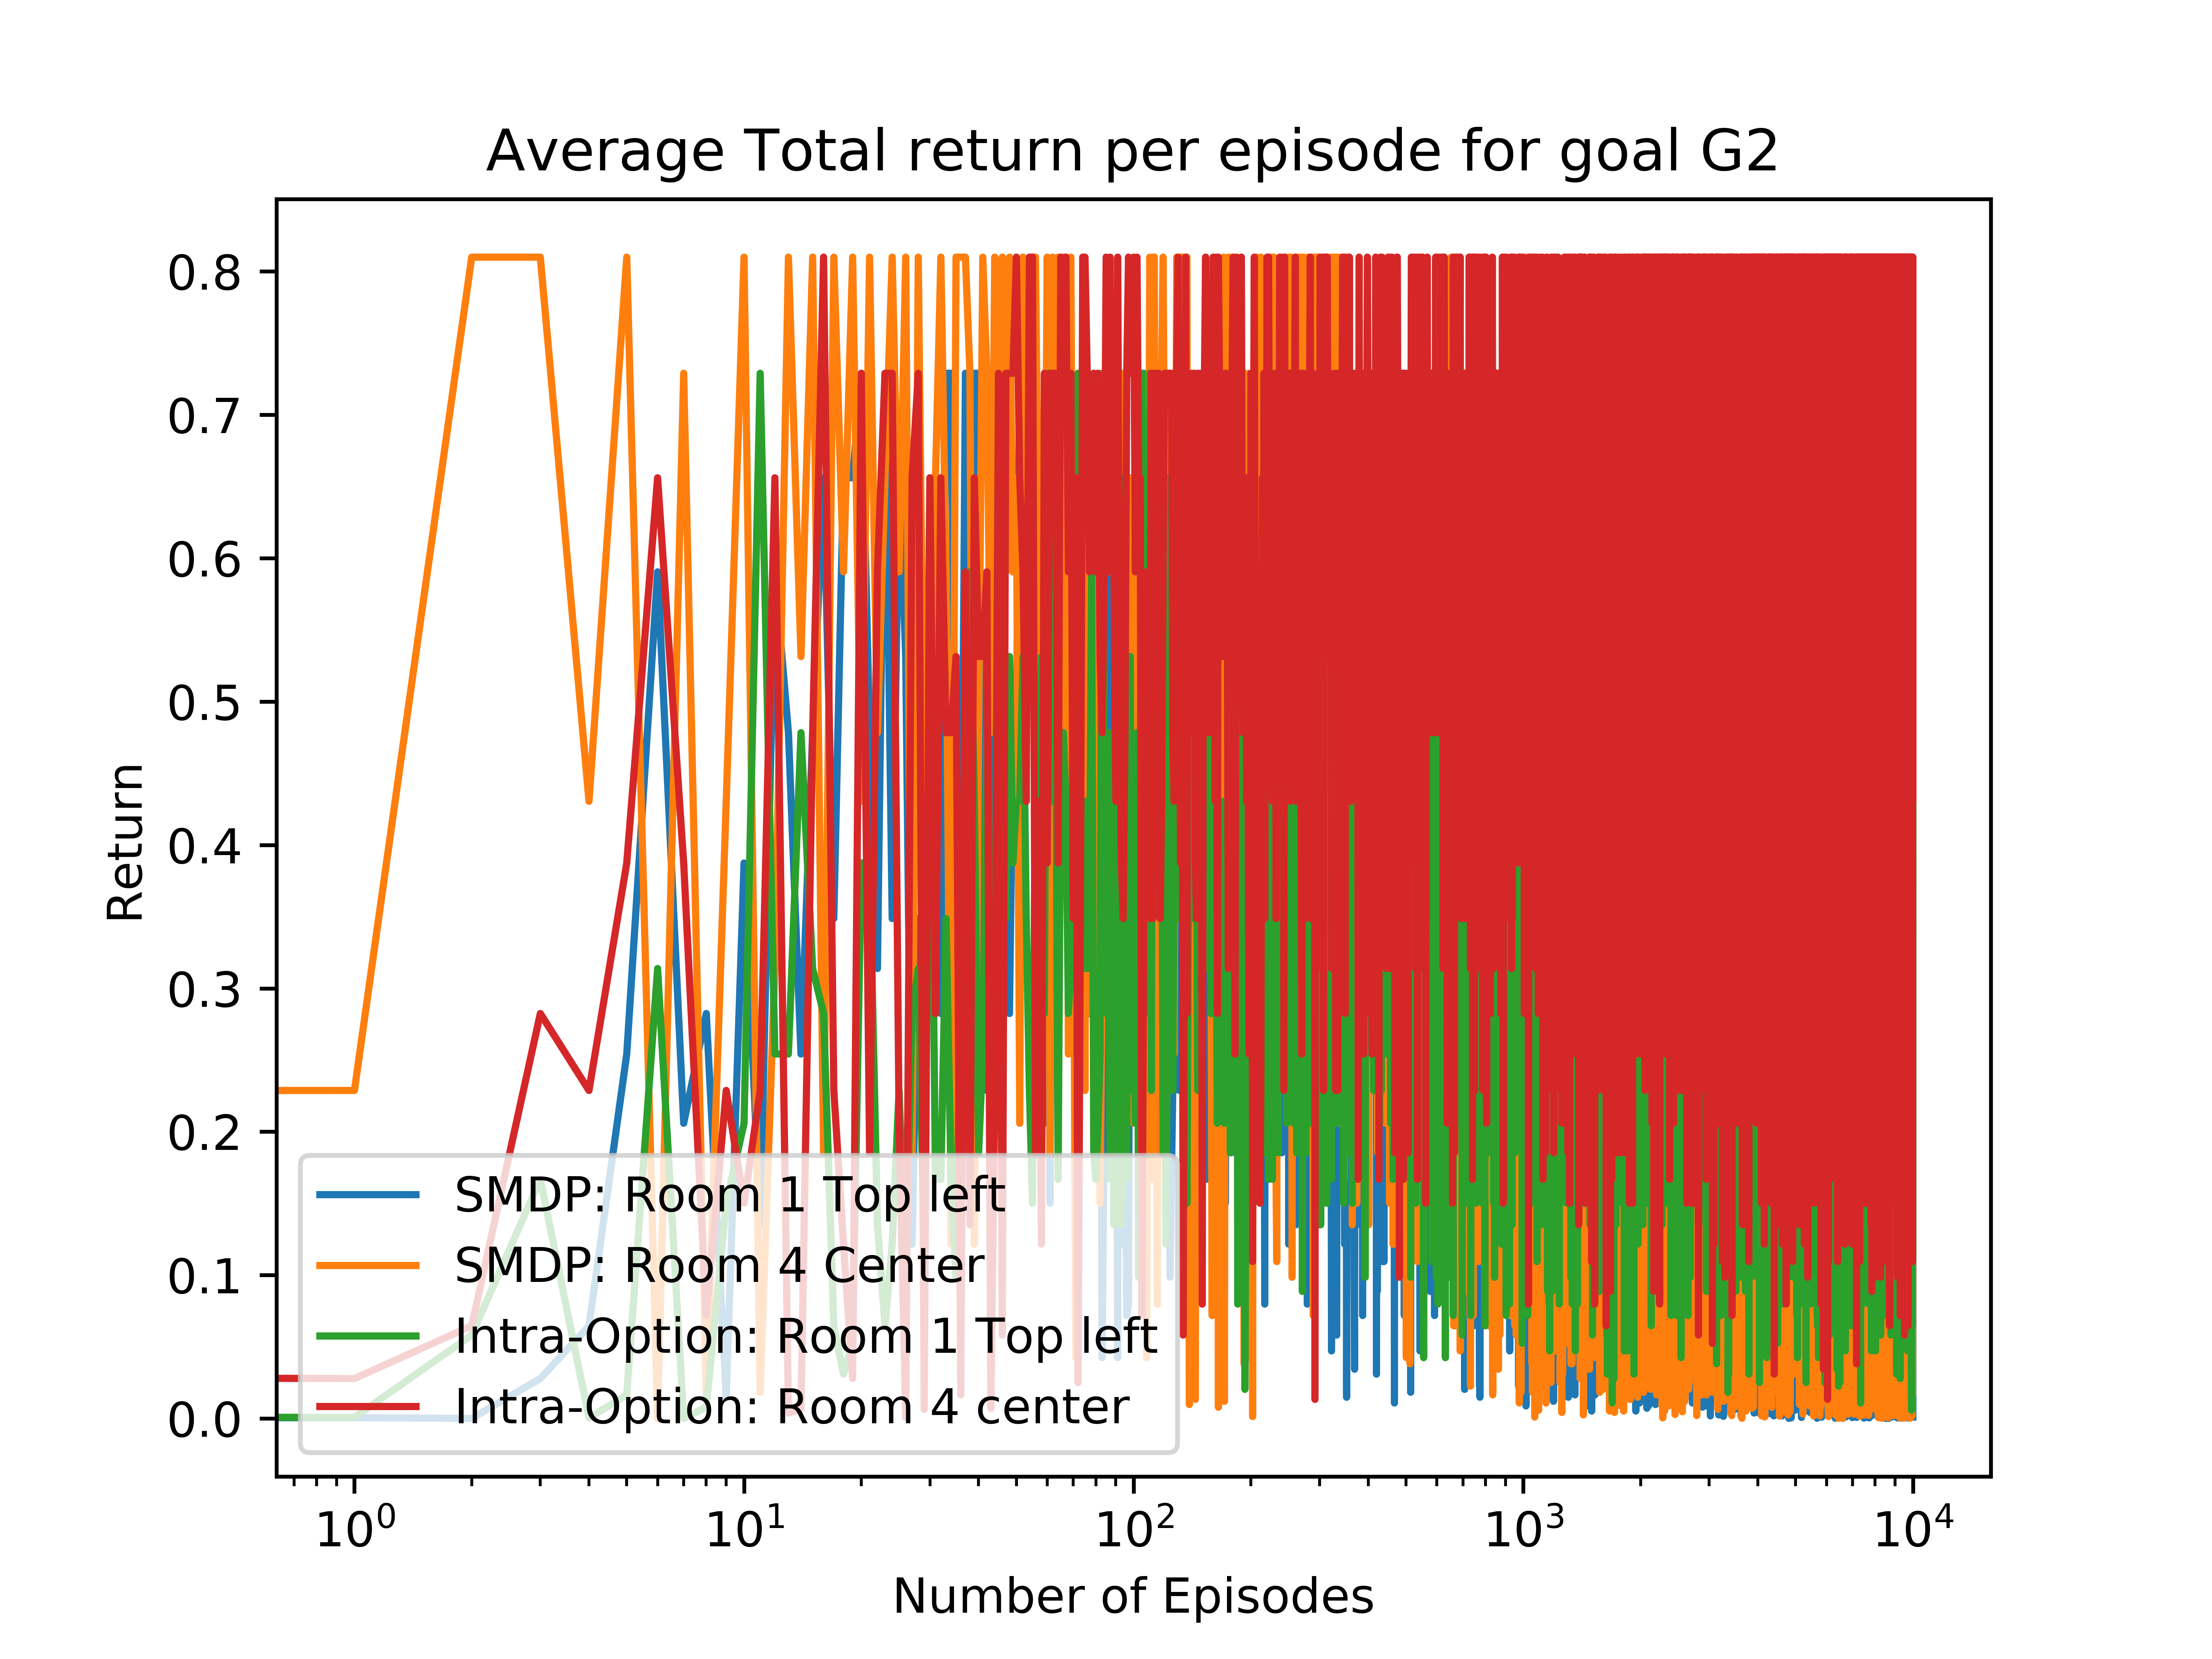
\includegraphics[width=0.4\linewidth]{./Total_return_G2.png}\label{option_G2}}
  	\caption{Average total return by SMDP and Intra-option Q learning for goal-G1 \ref{avg_steps_G1} and for goal-G2-\ref{avg_steps_G2}. Each option denotes the single step. The average is taken over 10 episodes and x-axis follows $\log 10$ scale.}
  	\label{fig:options}
  \end{figure}
 
 From fig.-\ref{fig:action} and fig.-\ref{fig:options}, it can be observed that \textbf{the average reward is higher for the case of Intra-option Q learning compared to SMDP. Variations in average reward is also slightly lower in case of intra-option Q leaning for the case of goal G1 and G2.}
 \newpage

\section{Deep Reinforcement Learning:}
 The downside of the reinforcement learning is instability for non-linear function. In some cases due to correlation in the observations, small change in Q value may adversely affect the target values and policy. Use of neural network with reinforcement learning to represent Q values can also change diverge the learning.
 
 To improve the stability of  reinforcement learning with neural network, \textbf{deep neural network(CNN)} can be used with experience reply. The role of  reinforcement learning is to reduce the correlation in the training set, by which learning can be smooth and variance can be reduced. Along with experience reply \textbf{target network} also play major role in stabilization of learning. Rather than computing the gradient of value function, target network can be used for generating $\hat{Q}$ from cloning of Q which can be used for learning targets $y_j$. This method can reduce the correlation.
 
 The loss function for DQn can be define as,
 \begin{equation}
 	L_i(\theta_i)  = E{s,a,r,s'}[(r+\gamma \max_{a'} Q(s',a',\theta_i) - Q(ss,a,\theta_i)^2]
 \end{equation} 
	
\subsection{Answers-1: Hyper-parameters and Learning Curve}	

  \begin{figure}[H]
  	\centering  
  	\subfigure
  	{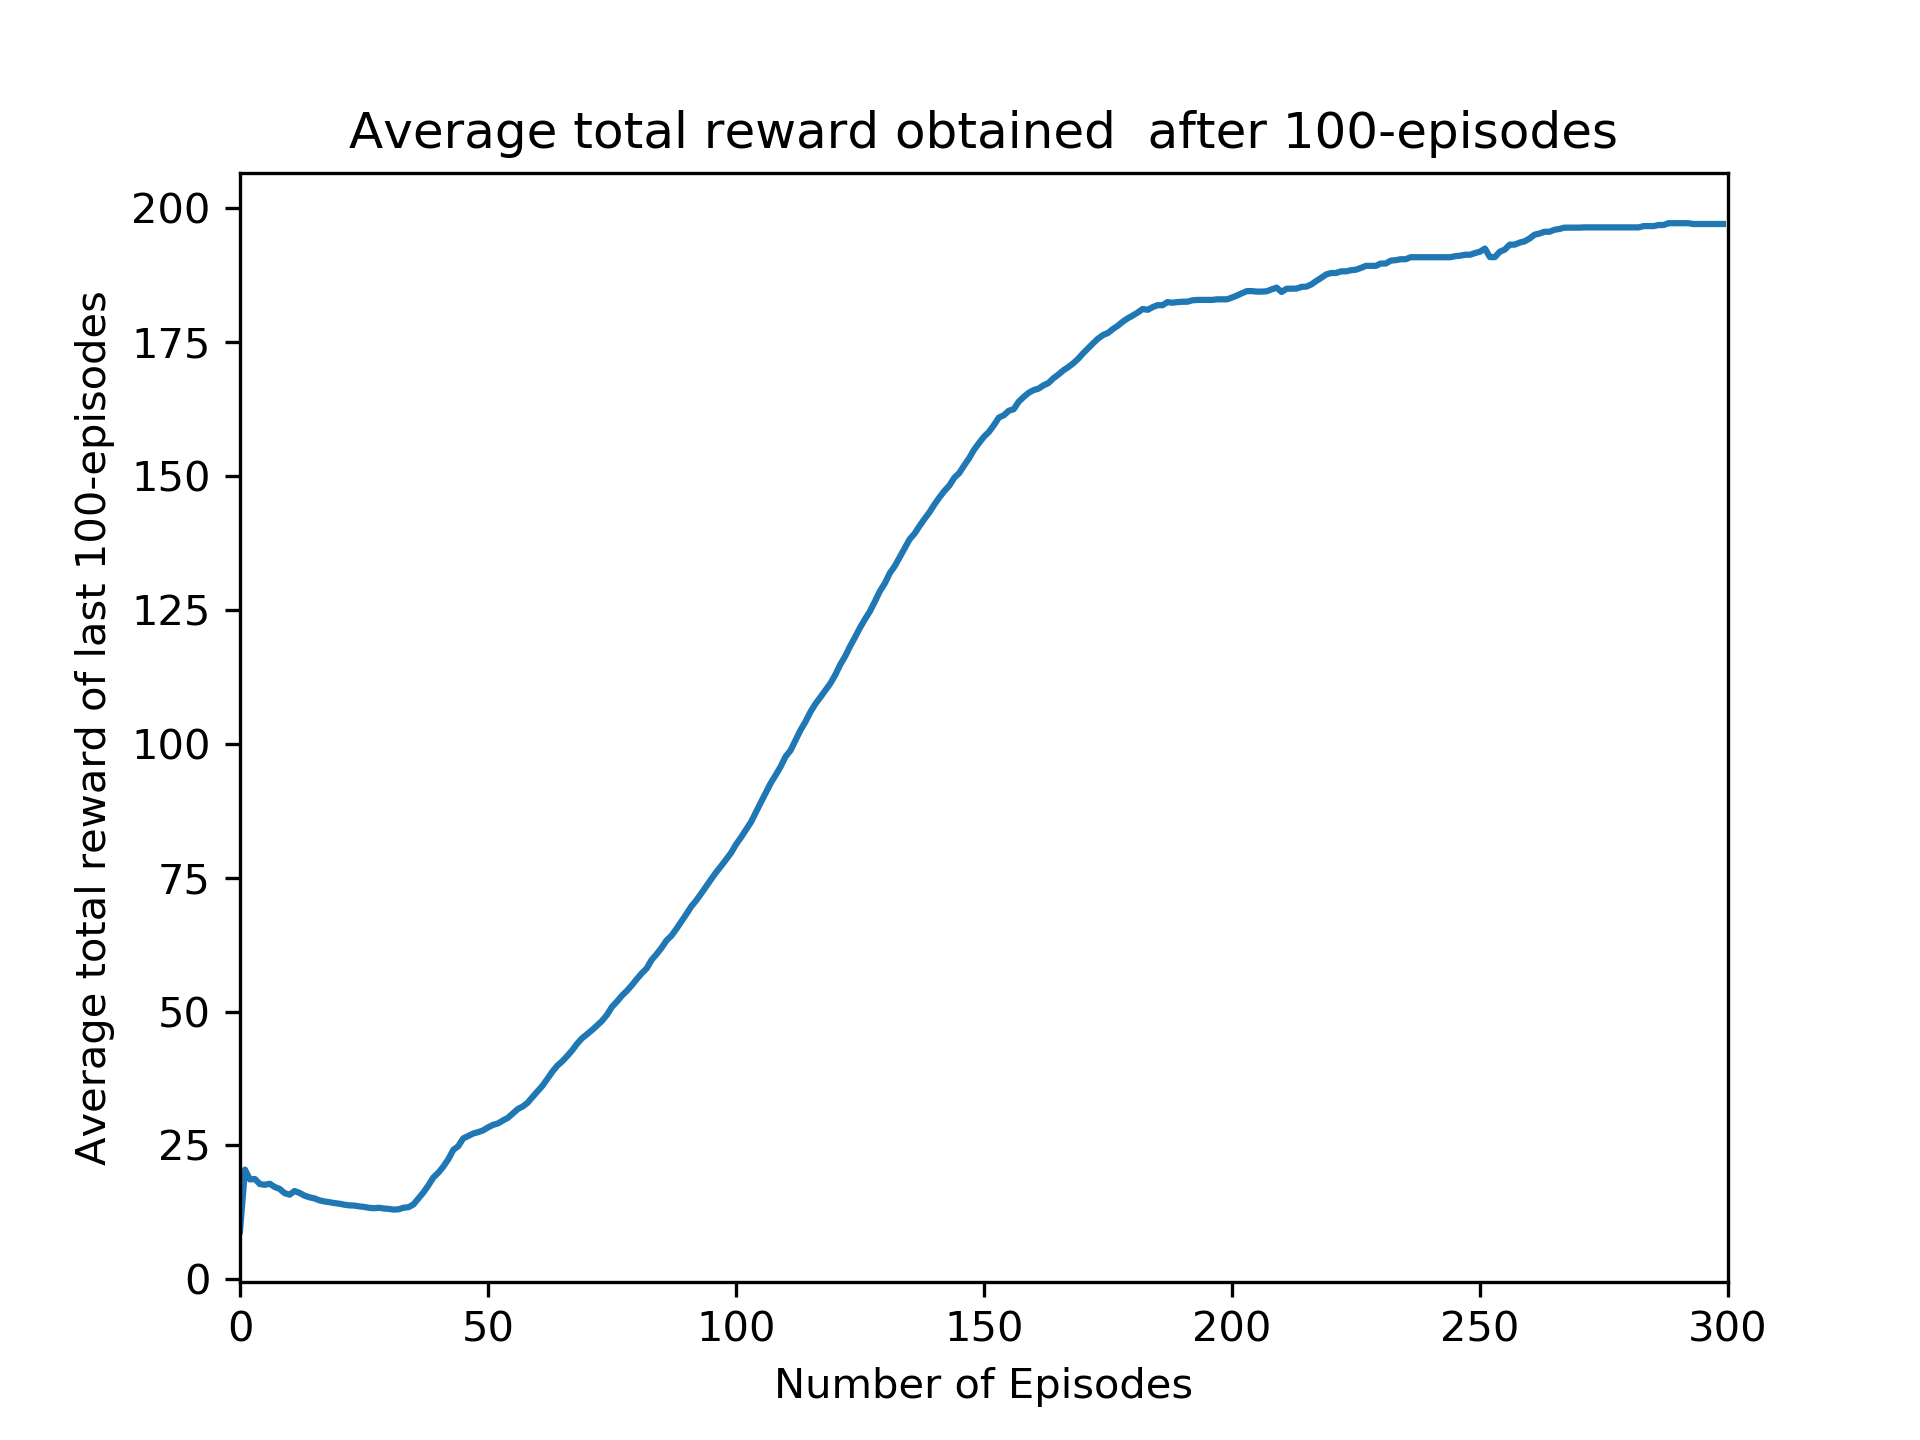
\includegraphics[width=0.4\linewidth]{./Avg_rewards.png}\label{re_simple_DQN}}
  	\subfigure
 	{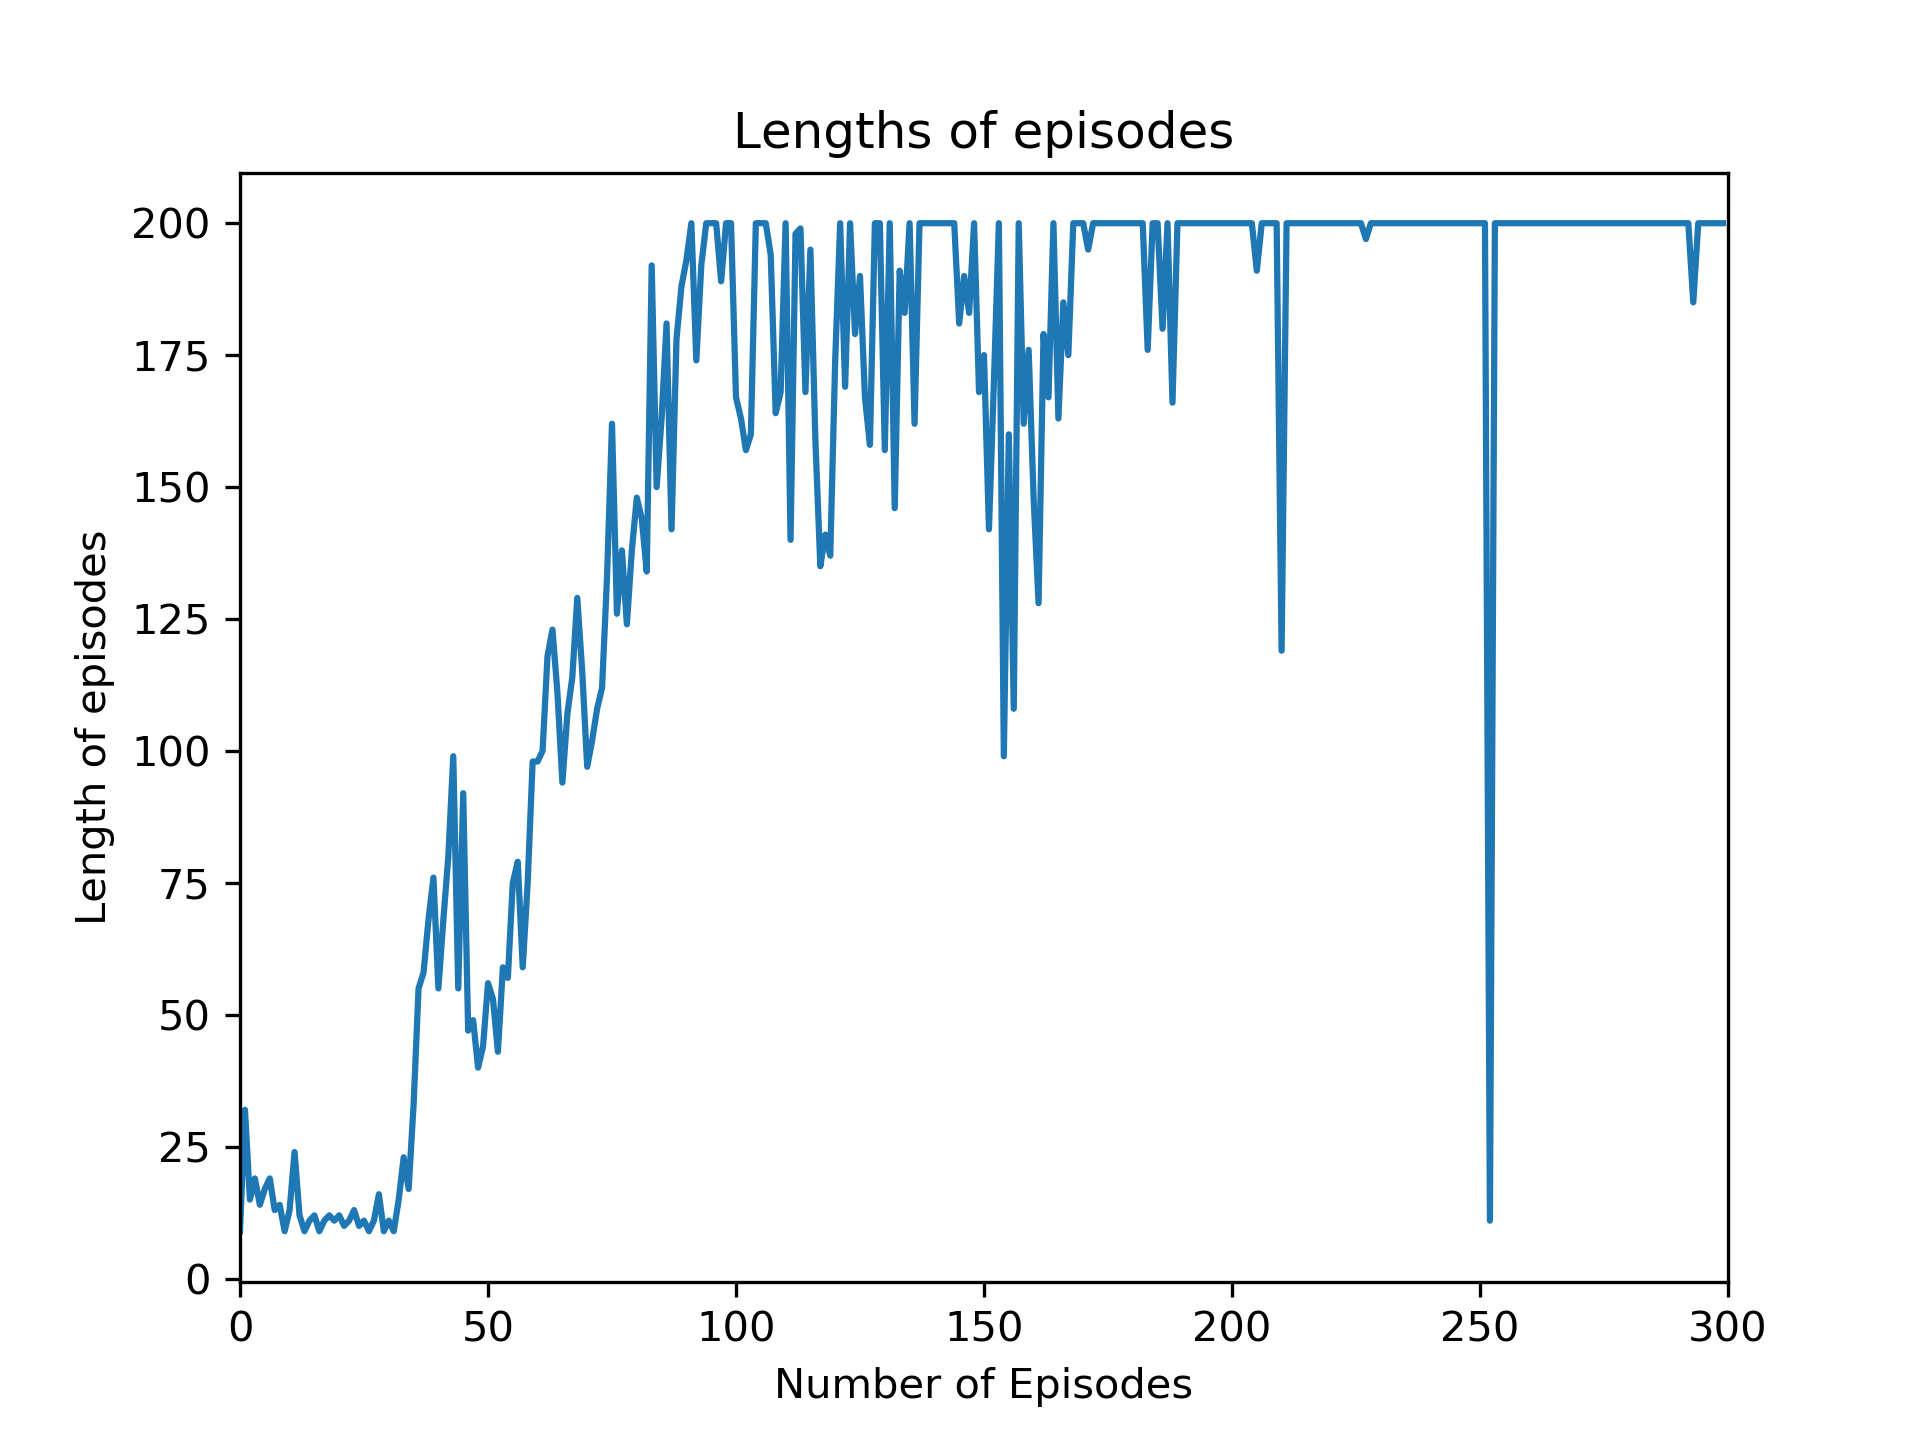
\includegraphics[width=0.4\linewidth]{./Episode_lengths.png}\label{epi_simple_DQN}}
  	\subfigure
	{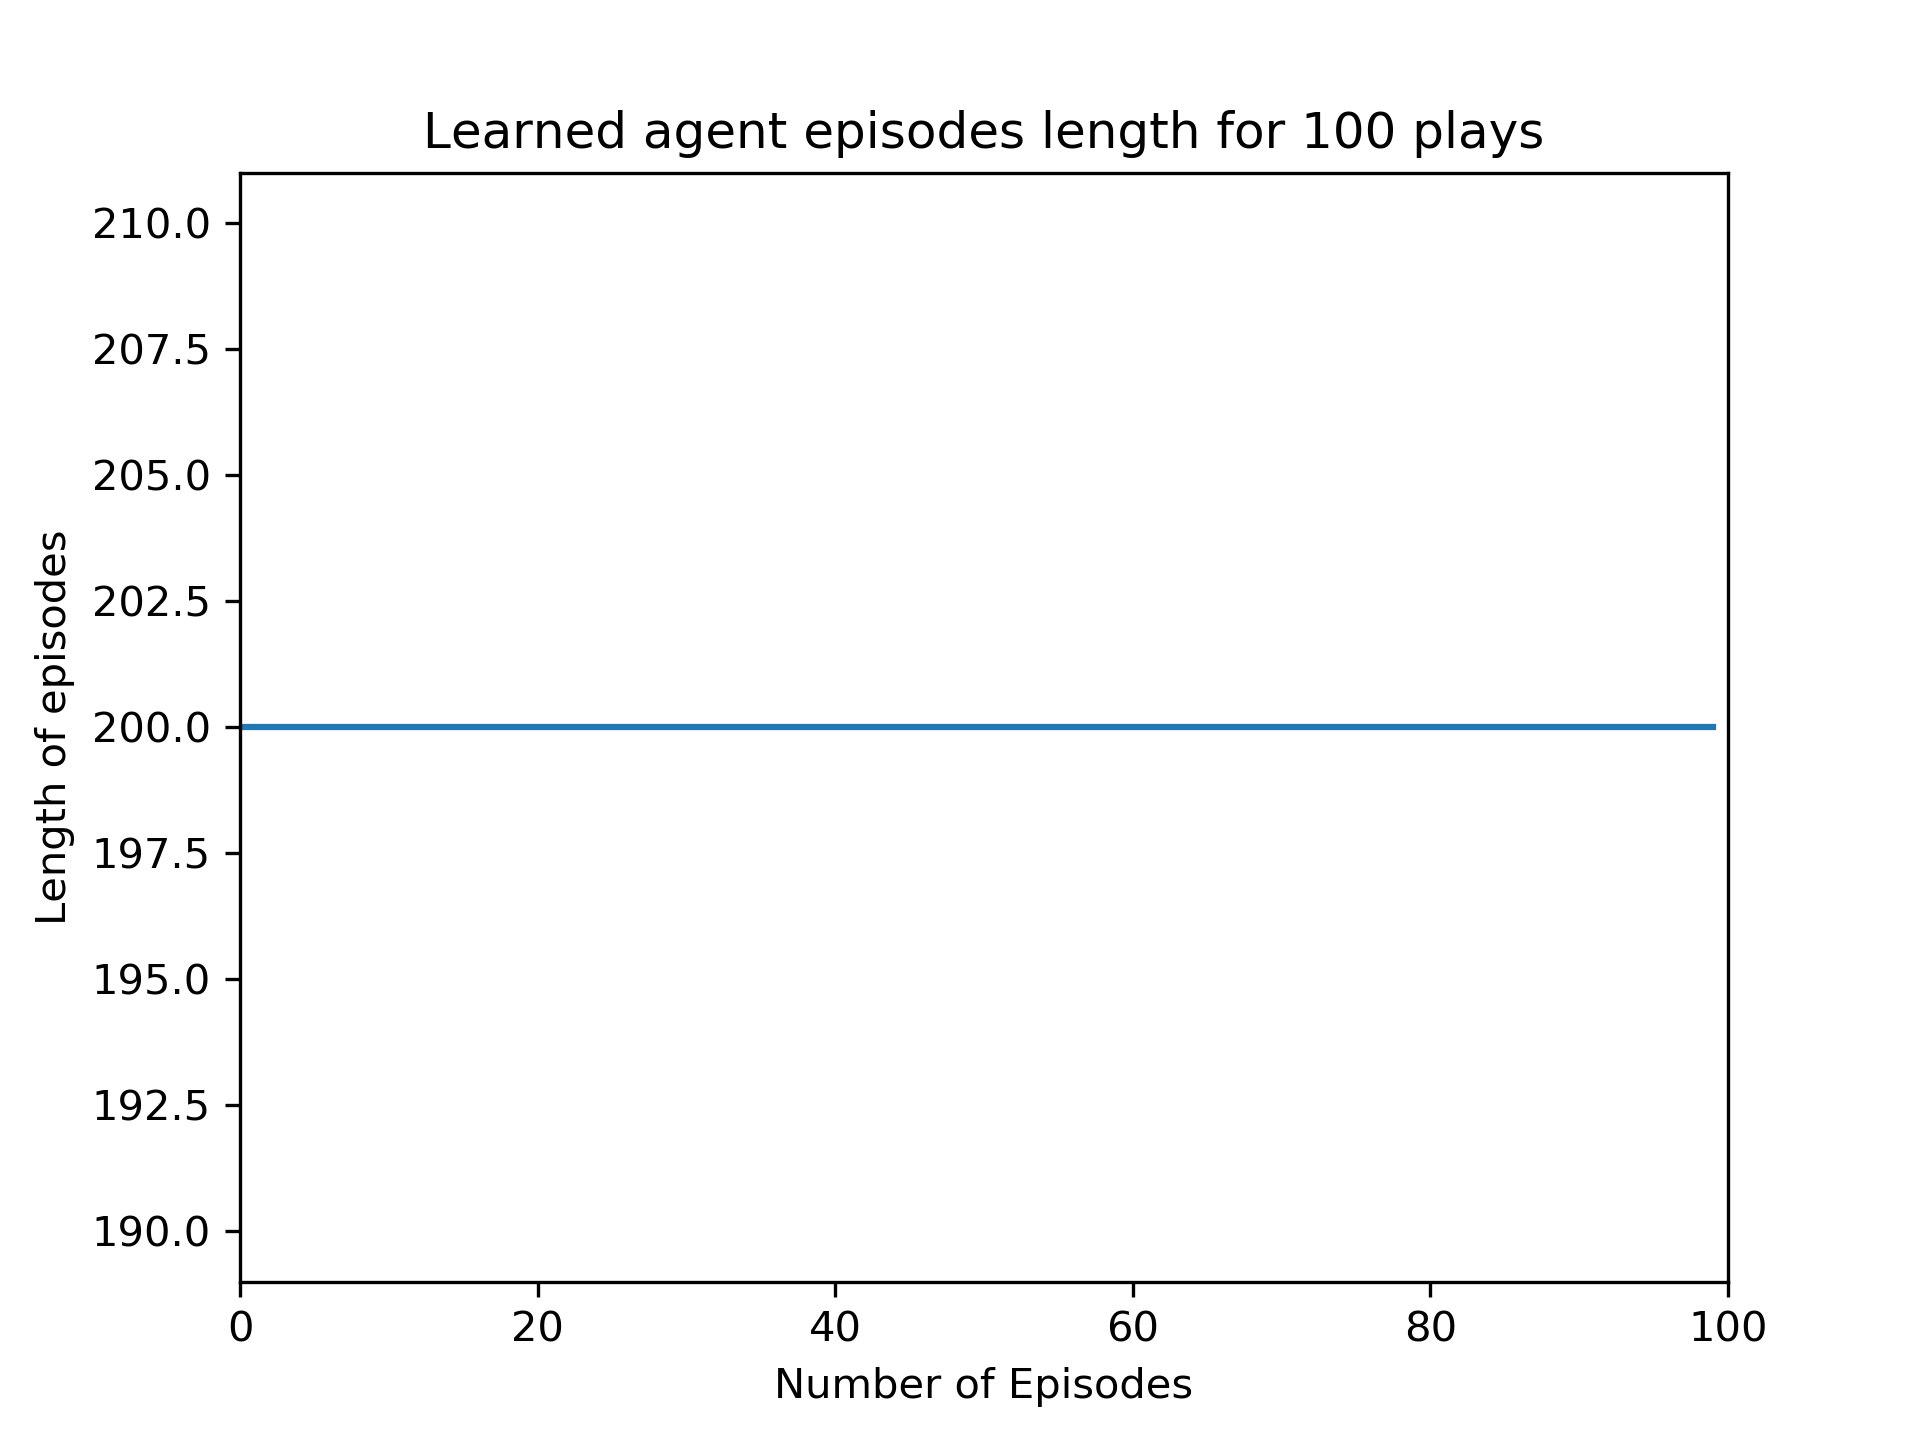
\includegraphics[width=0.4\linewidth]{./Learned_Episode_lengths.png}\label{ler_simple_DQN}}
  	\caption{Plots of Average total reward of last 100 episode \ref{re_simple_DQN}, episode length \ref{epi_simple_DQN}, learned agent episode length \ref{ler_simple_DQN}}
  	\label{fig:simple}
  \end{figure}
  
  The goal is to train the DQN such that it gives average reward for cart-pole should be more than 200 which is obtain as given in fig.-\ref{re_simple_DQN}. Figure-\ref{re_simple_DQN} indicates that performance agent is poor in initial stage due to set of $\epsilon$=1 and slow decay rate 0.995. After certain period of exploration, agent learned the optimal policy which can be concluded from figure-\ref{re_simple_DQN}. Till 180 episodes maximum reward obtained is 175, whereas after around 200 episodes agent has learned the optimal policy and has obtained reward around 190 to 200 for next 100 episodes. Similar observation can be concluded from the length of episode plot. 
  
  Around 50 episodes there is lot of fluctuation in episode length which reduces till 200. After 200 episode there is almost no fluctuation in result which is indication of learned optimal policy. Figure-\ref{ler_simple_DQN} indicates the episode length after 200 episodes. The constant vales indicates optimal policy.

\subsection{Answers-2: Report of hyper-parameters tuning}

The set of hyper parameter which worked best for cart-pole problem is given in table-\ref{tab:hyperPara}.

\begin{table}[H]
	\begin{tabular}{|c|c|c|}
		\hline
		\textbf{Hyperparameters} & \textbf{Value} & \textbf{Description} \\ \hline
		Initial Epsilon & 1 & Start value of $\epsilon $ for exploration \\ \hline
		Epsilon Decay Rate & 0.995 & Decay Multiplier of $\epsilon$ \\ \hline
		Discount Factor & 0.99 & Discount factor for Q learning \\ \hline
		Max Steps & 200 & Maximum Number of steps for each episodes \\ \hline
		Episode Num & 300 & Count of Number of episodes for traning \\ \hline
		Target Update Freq & 200 & Number of steps after which target network has to be upated \\ \hline
		Minibatch Size & 32 & Size of batch samples taken from experience reply \\ \hline
		Learning rate & 0.001 & Learning rate Adam Solver \\ \hline
		Reply Memory Size & 10000 & Size of reply memory \\ \hline
		Regularization Factor & 0.0001 & Regularization factor for overfitting \\ \hline
		Min Epsilon & 0.01 & Minimum value $\epsilon$ can achieve after decay \\ \hline
		Hidden1 Size & 20 & Size of neural network for Hidden layer - 1 \\ \hline
		Hidden2 Size & 20 & Size of neural network for Hidden layer - 2 \\ \hline
		Hidden3 Size & 20 & Size of neural network for Hidden layer - 3 \\ \hline
	\end{tabular}
	\vspace{1mm}
	\caption{Set of Hyperparameters}
	\label{tab:hyperPara}
\end{table}


\newpage

\subsection{Answers-3: Report of the variation of hyper-parameters like hidden layer sizes, epsilon, mini-batch size, target frequency.}  
	
	        \begin{figure}[H]
	        	\centering  
	        	\subfigure
	        	{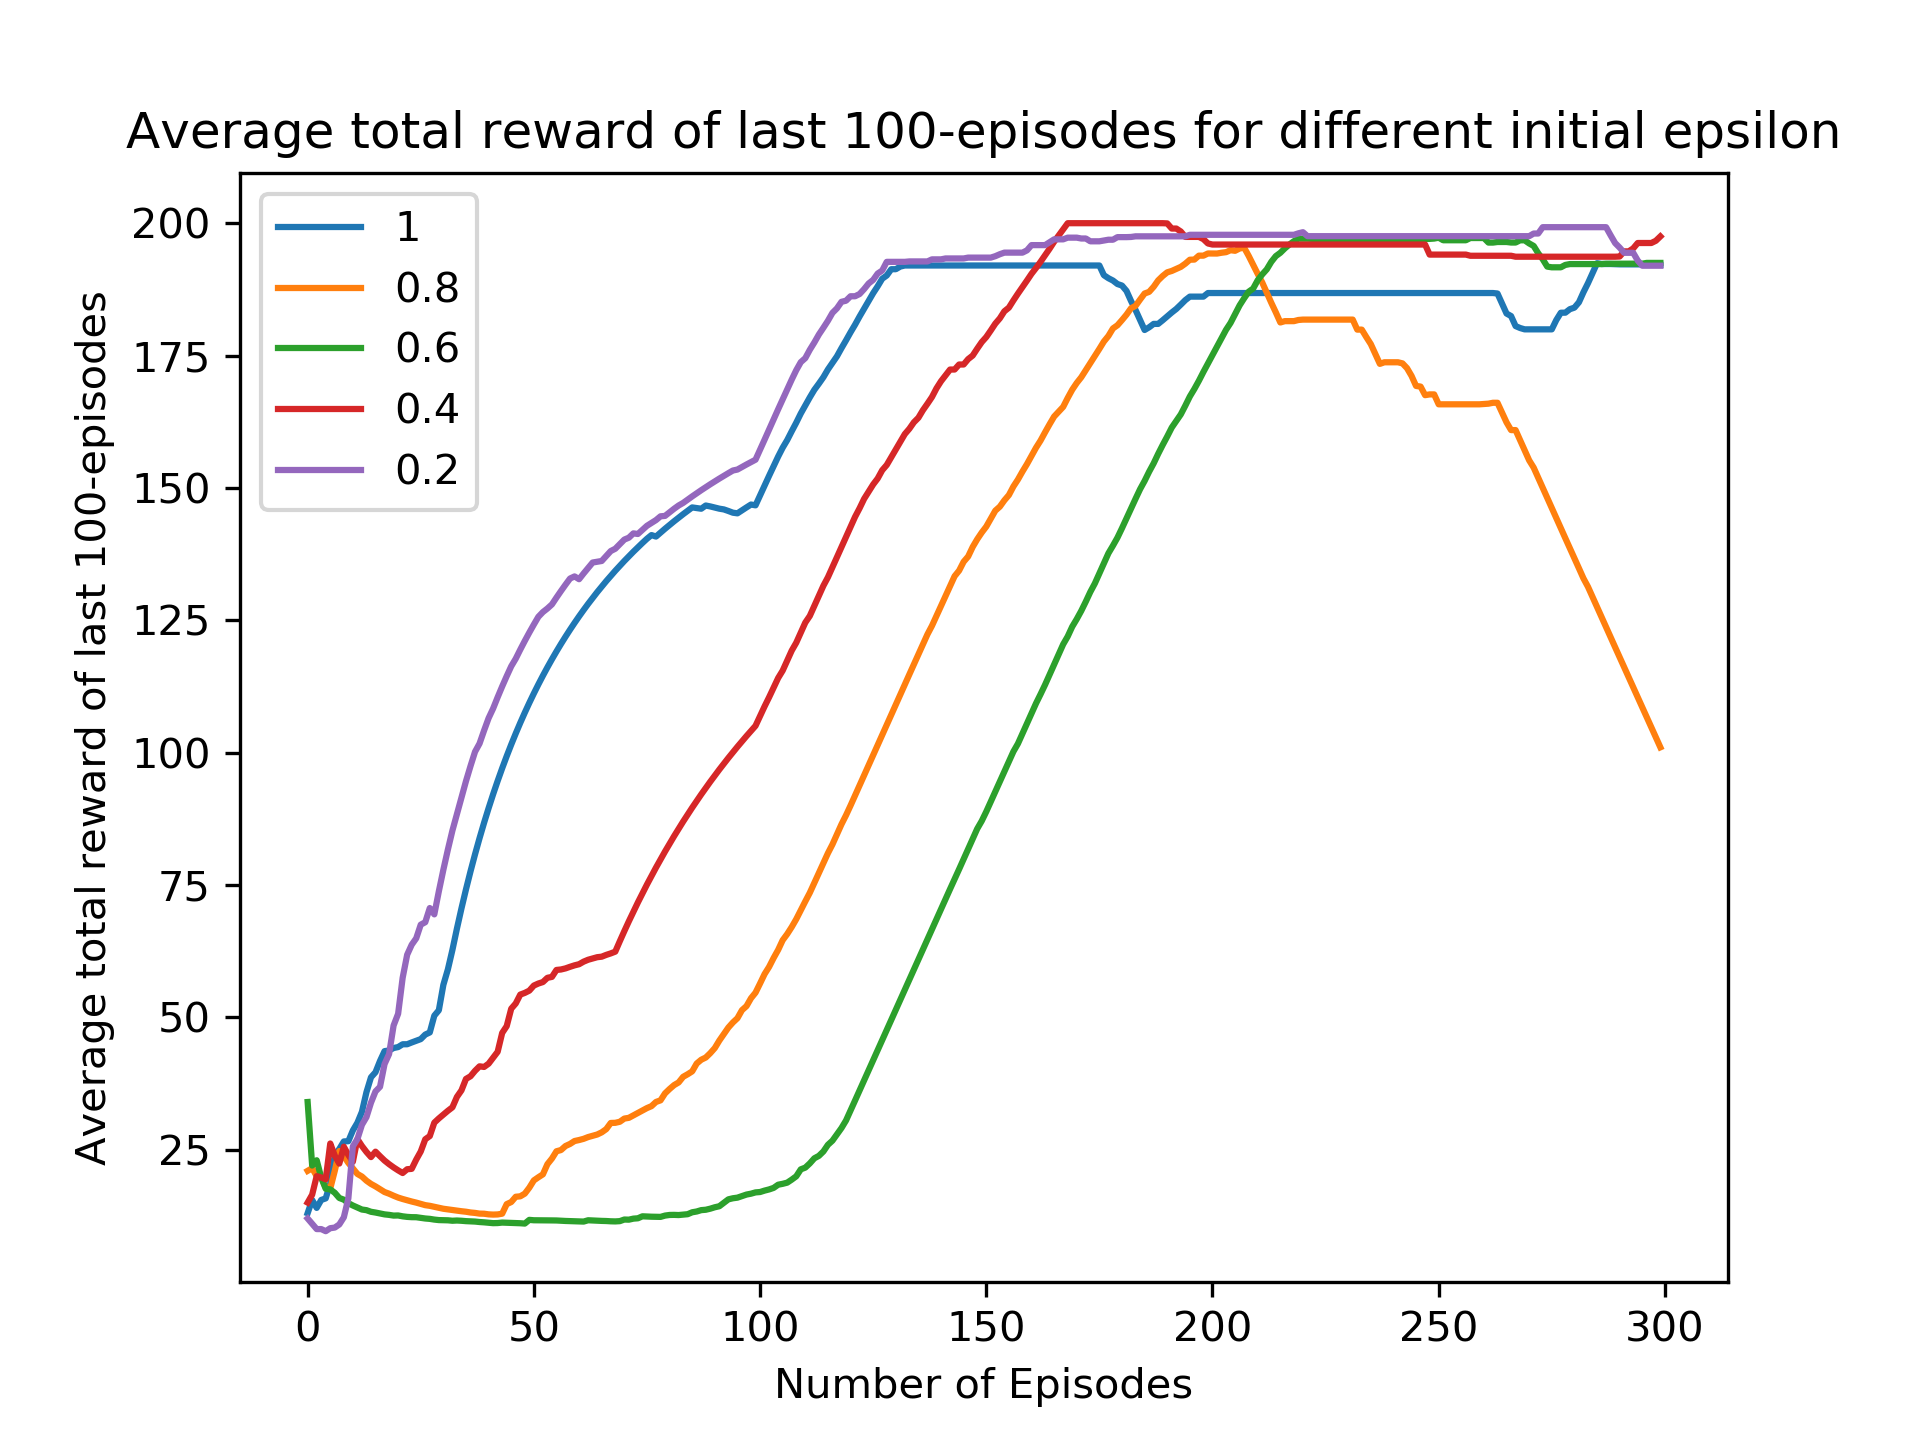
\includegraphics[width=0.4\linewidth]{./Avg_rewards_EPSILONs.png}\label{epsilon}}
	        	\subfigure
	        	{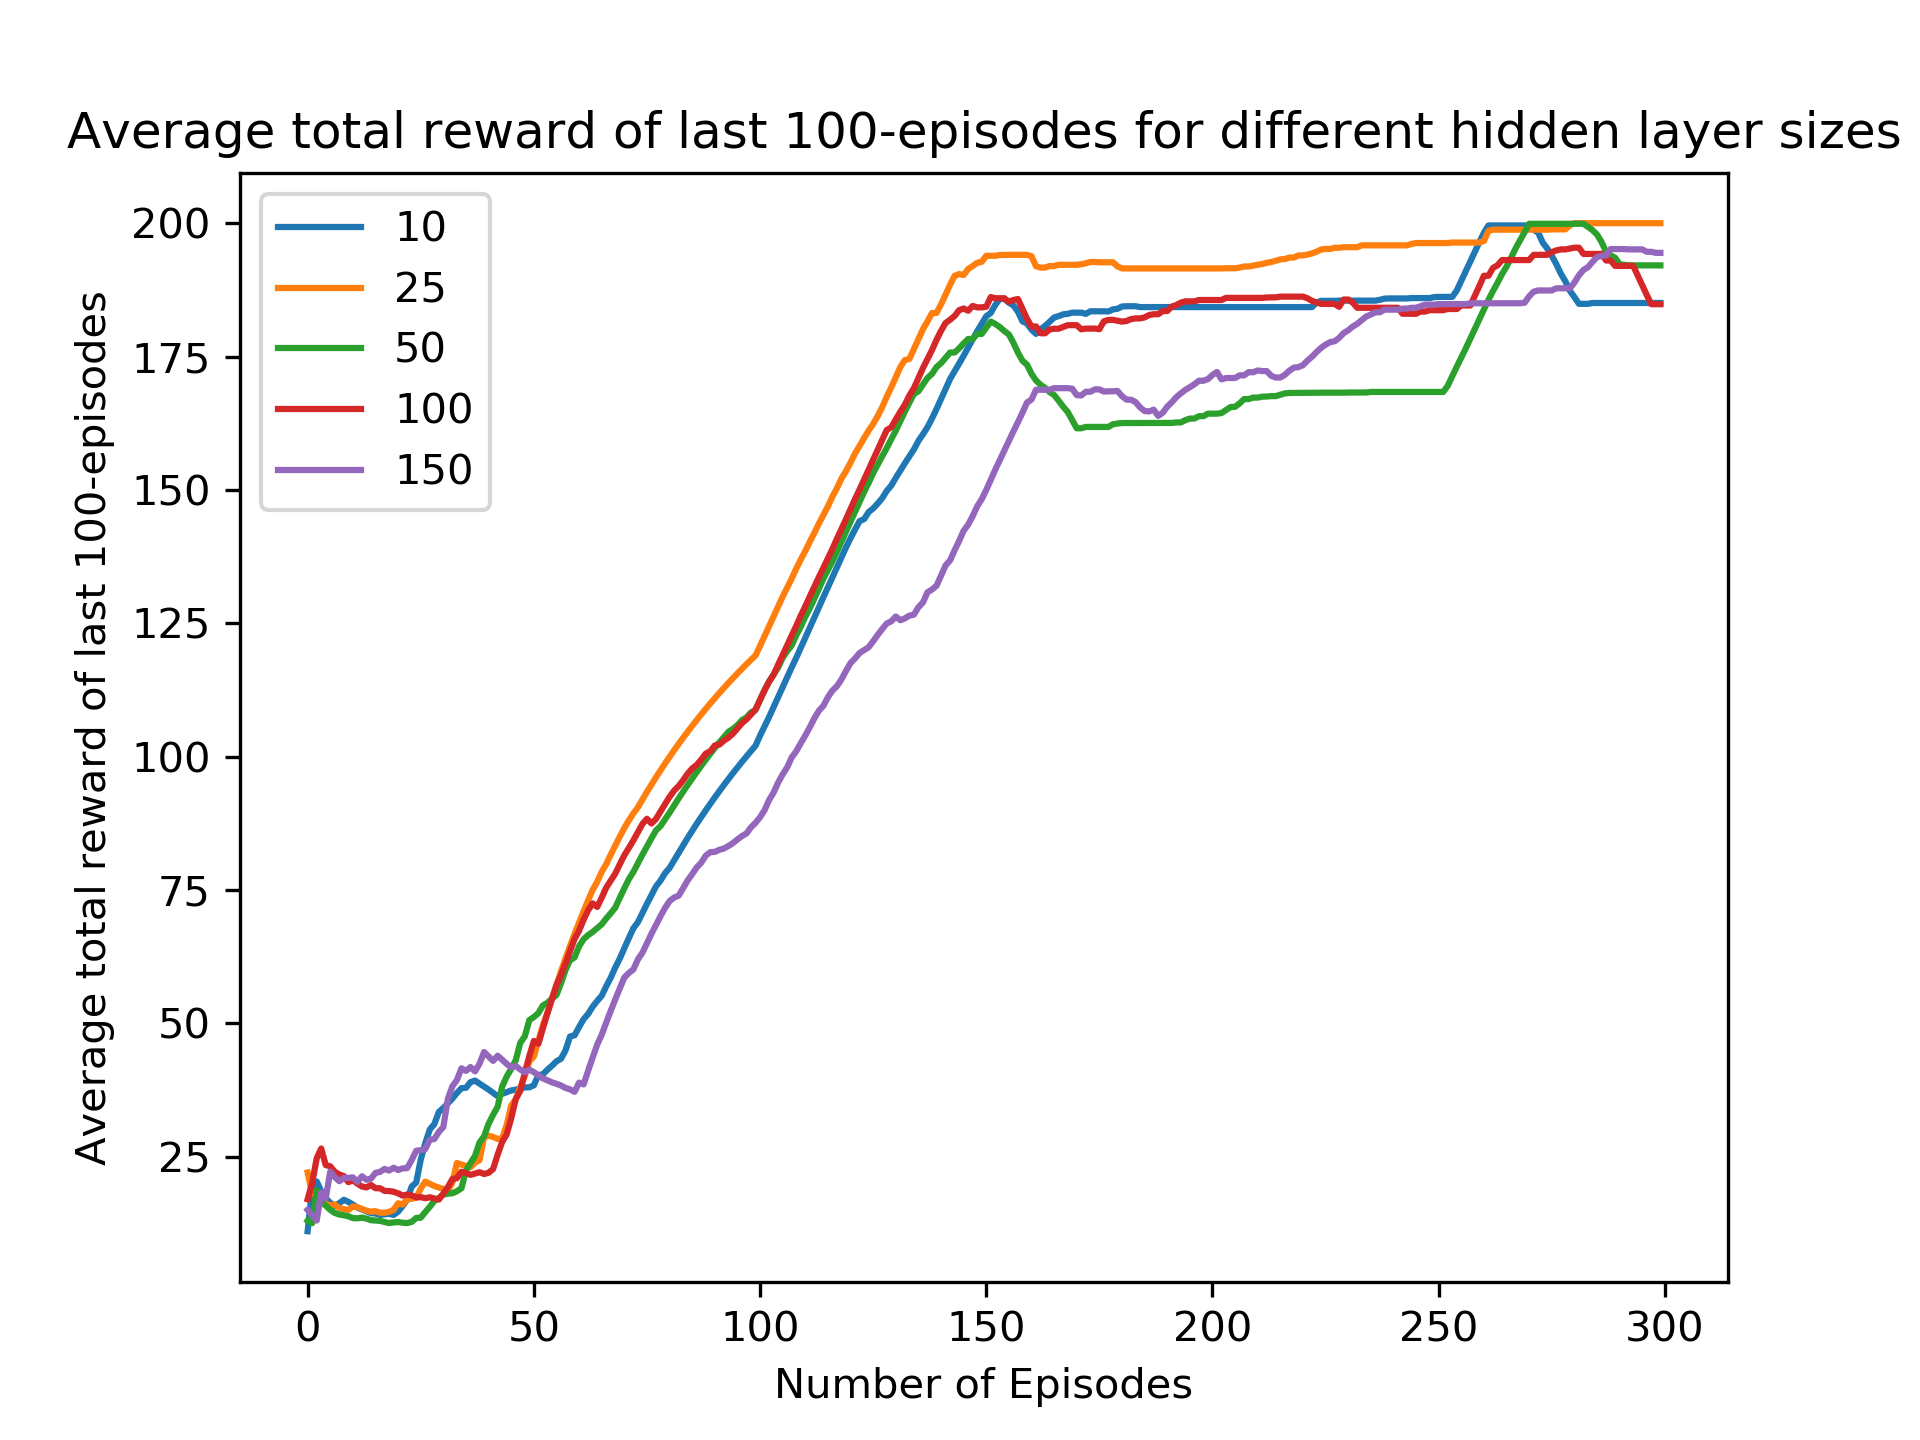
\includegraphics[width=0.4\linewidth]{./Avg_rewards_HiddenSizes.png}\label{hidden}}
	        	\subfigure
	        	{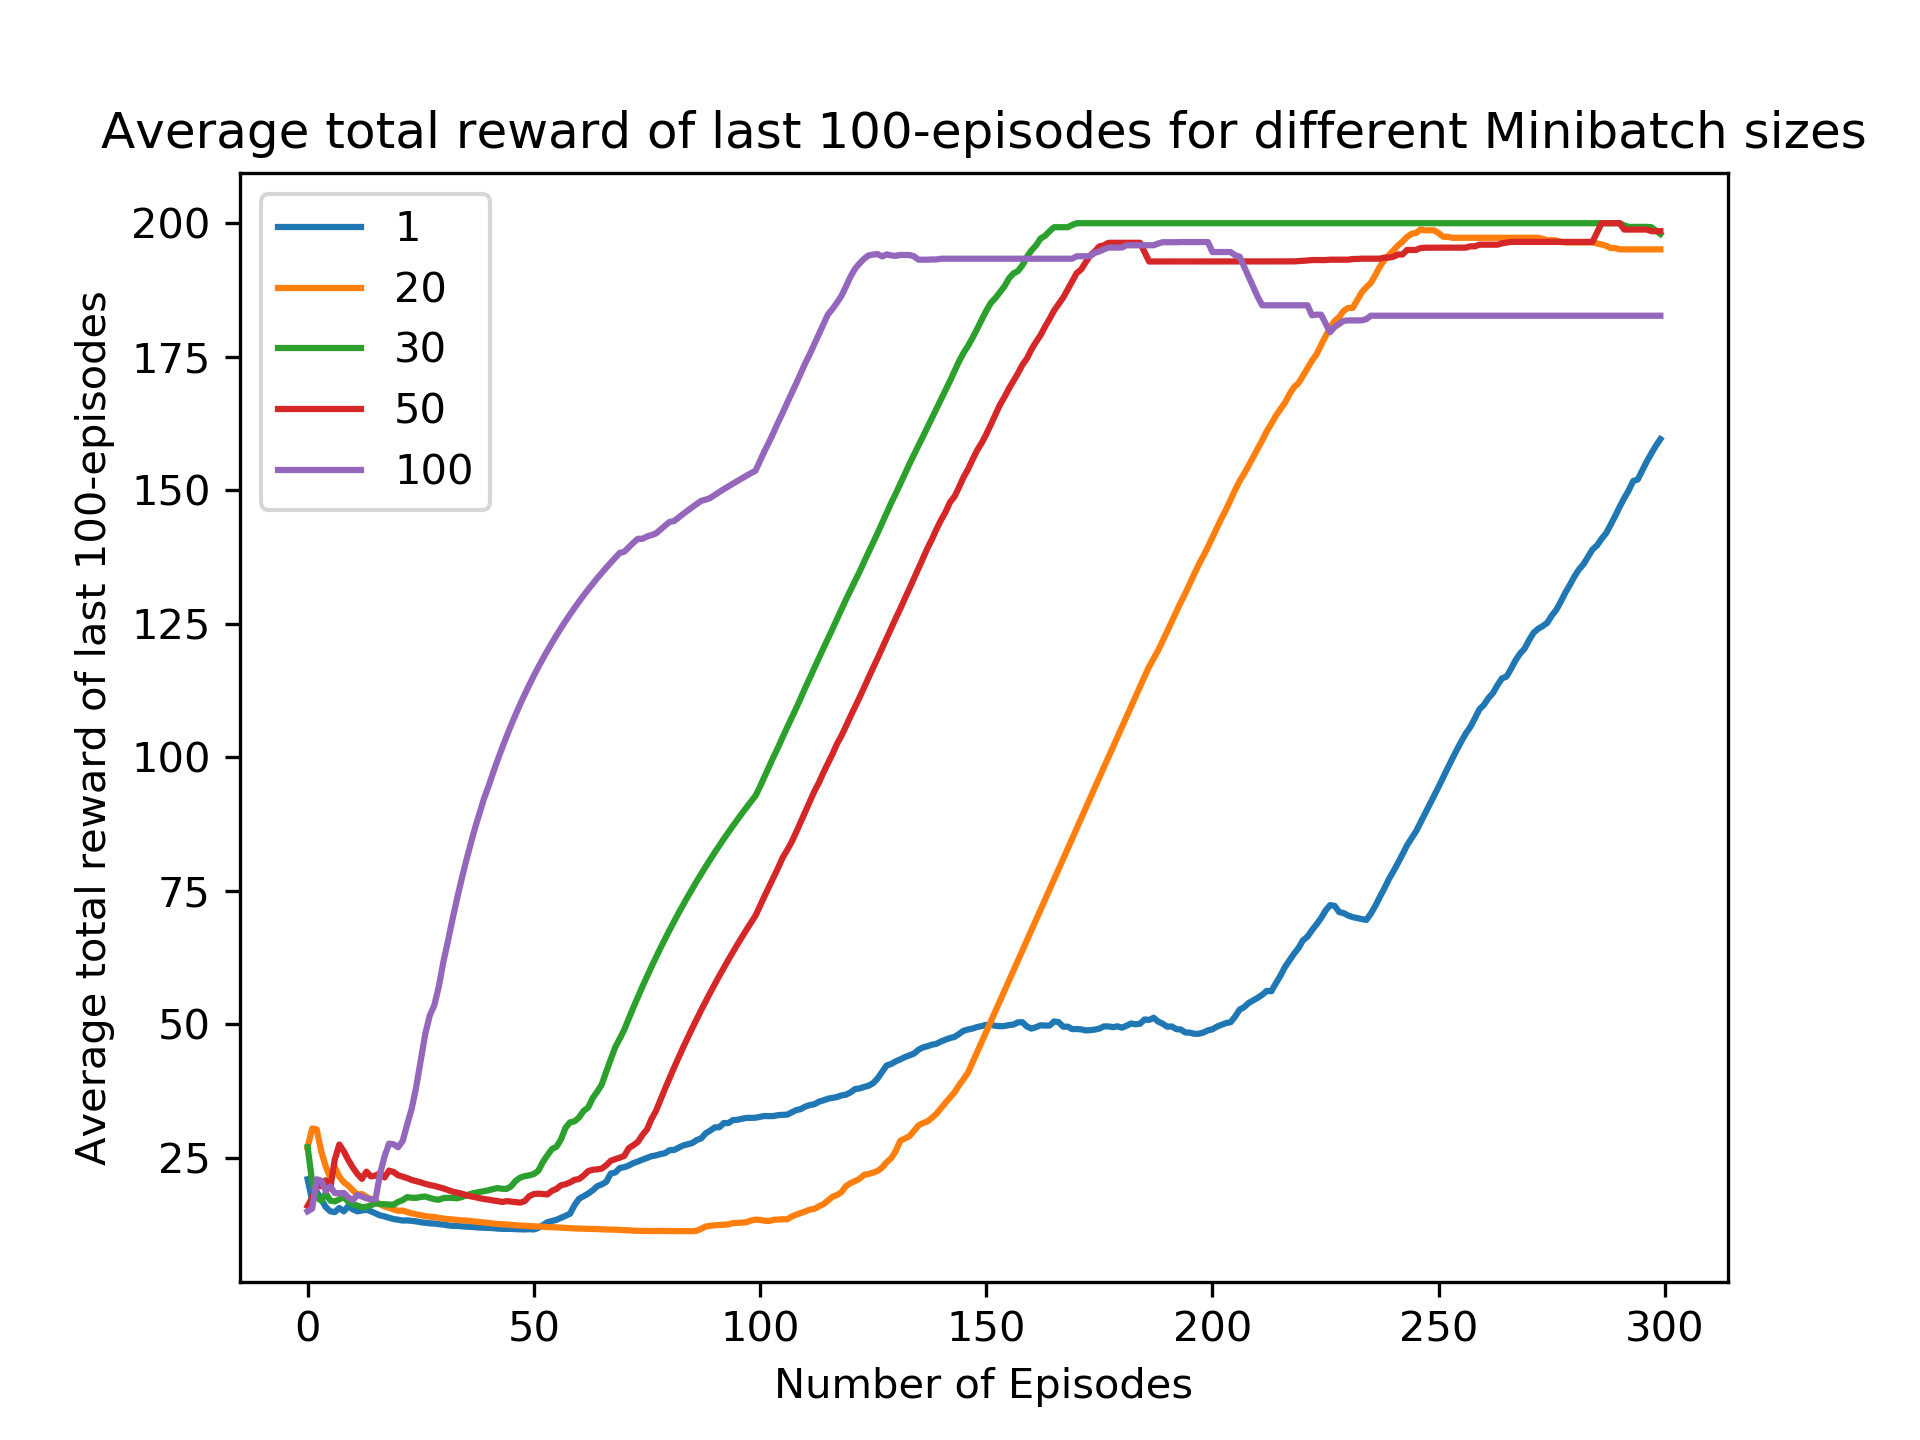
\includegraphics[width=0.4\linewidth]{./Avg_rewards_MINIBATCHs.png}\label{minibatch}}
	        	\subfigure
	        	{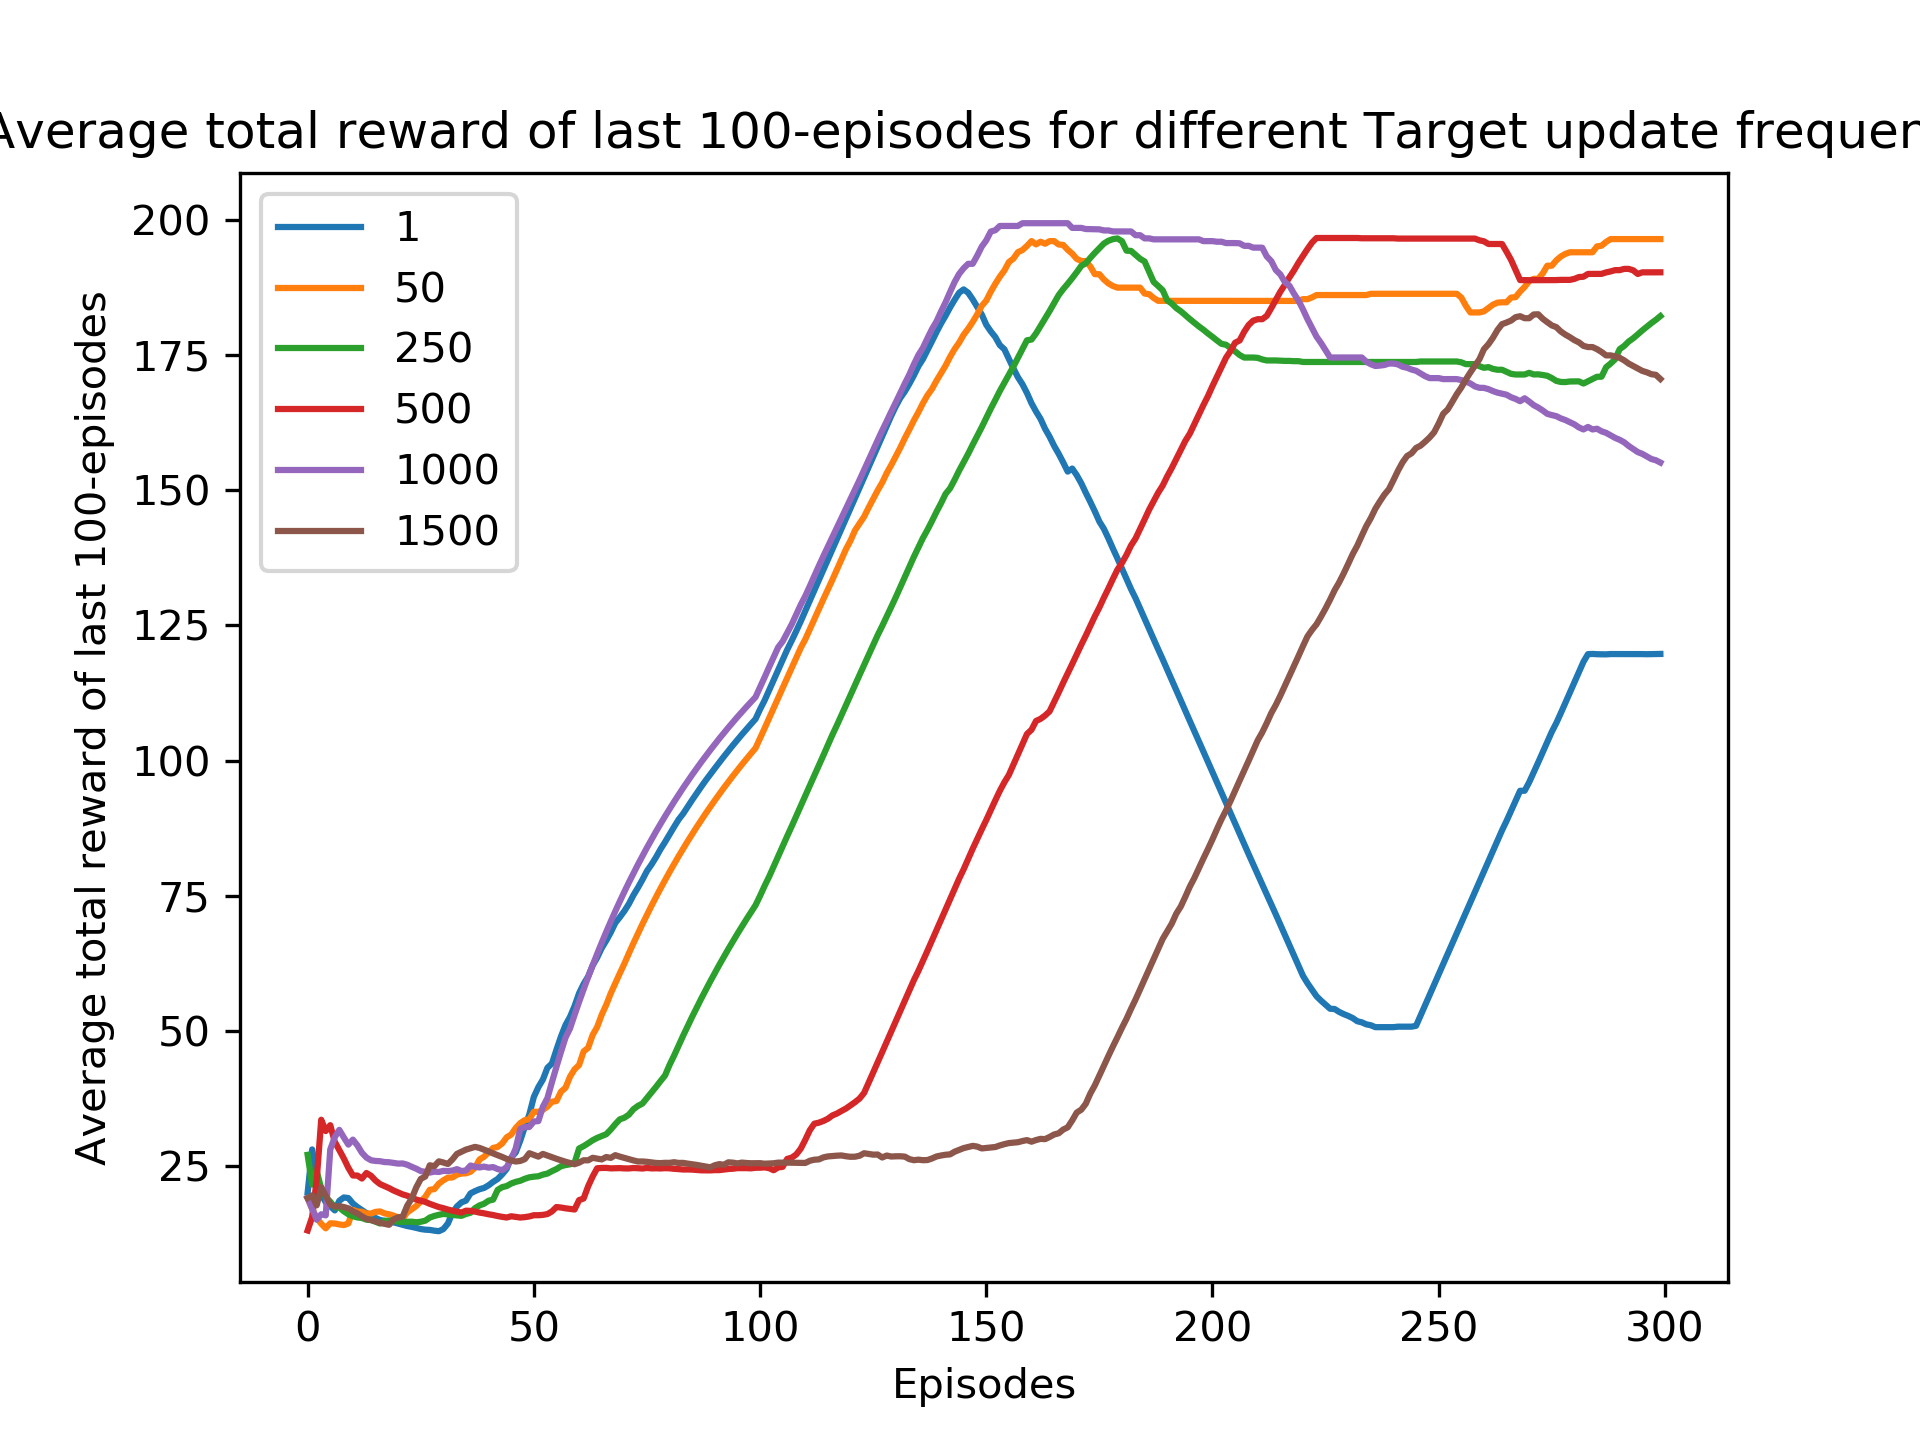
\includegraphics[width=0.4\linewidth]{./Avg_rewards_TARGETs.png}\label{target}}
	        	\caption{Comparative plots of learning curves of different hyper parameters : Initial value of epsilon-\ref{epsilon}, Hidden layers-\ref{hidden}, size of minibatch-\ref{minibatch}, update frequency of target networks-\ref{target}}
	        	\label{hyper}
	        \end{figure}
	 
	 The comparative plots of different hyper-parameters and its different values are given in fig.-\ref{hyper}. The initial value of $\epsilon$ is selected as \textbf{\{1, 0.8, 0.6, 0.4, 0.2\}.} For very high value(1) and small value (0.2), the agent learns policy faster and its gains the average reward of 200. For high value of $\epsilon$, agent does much exploration which helps to learn optimal policy faster. Whereas, for very small value of $\epsilon$, the greedy behavior causes the to learn optimal policy faster.
	 
	  But in both cases transition has fluctuation. For value of 0.8, due to exploration there is slight decline is average reward. For case of 0.4 result has slight fluctuation. But, \textbf{in case of $\epsilon = 0.6$ the average reward transition is intially slow due to exploration but slowly it stabilize and gives maximum average reward which gives overall smooth transition in the result.s}
	  
	  
 
    \begin{figure}[H]
    	\centering  
    	\subfigure
    	{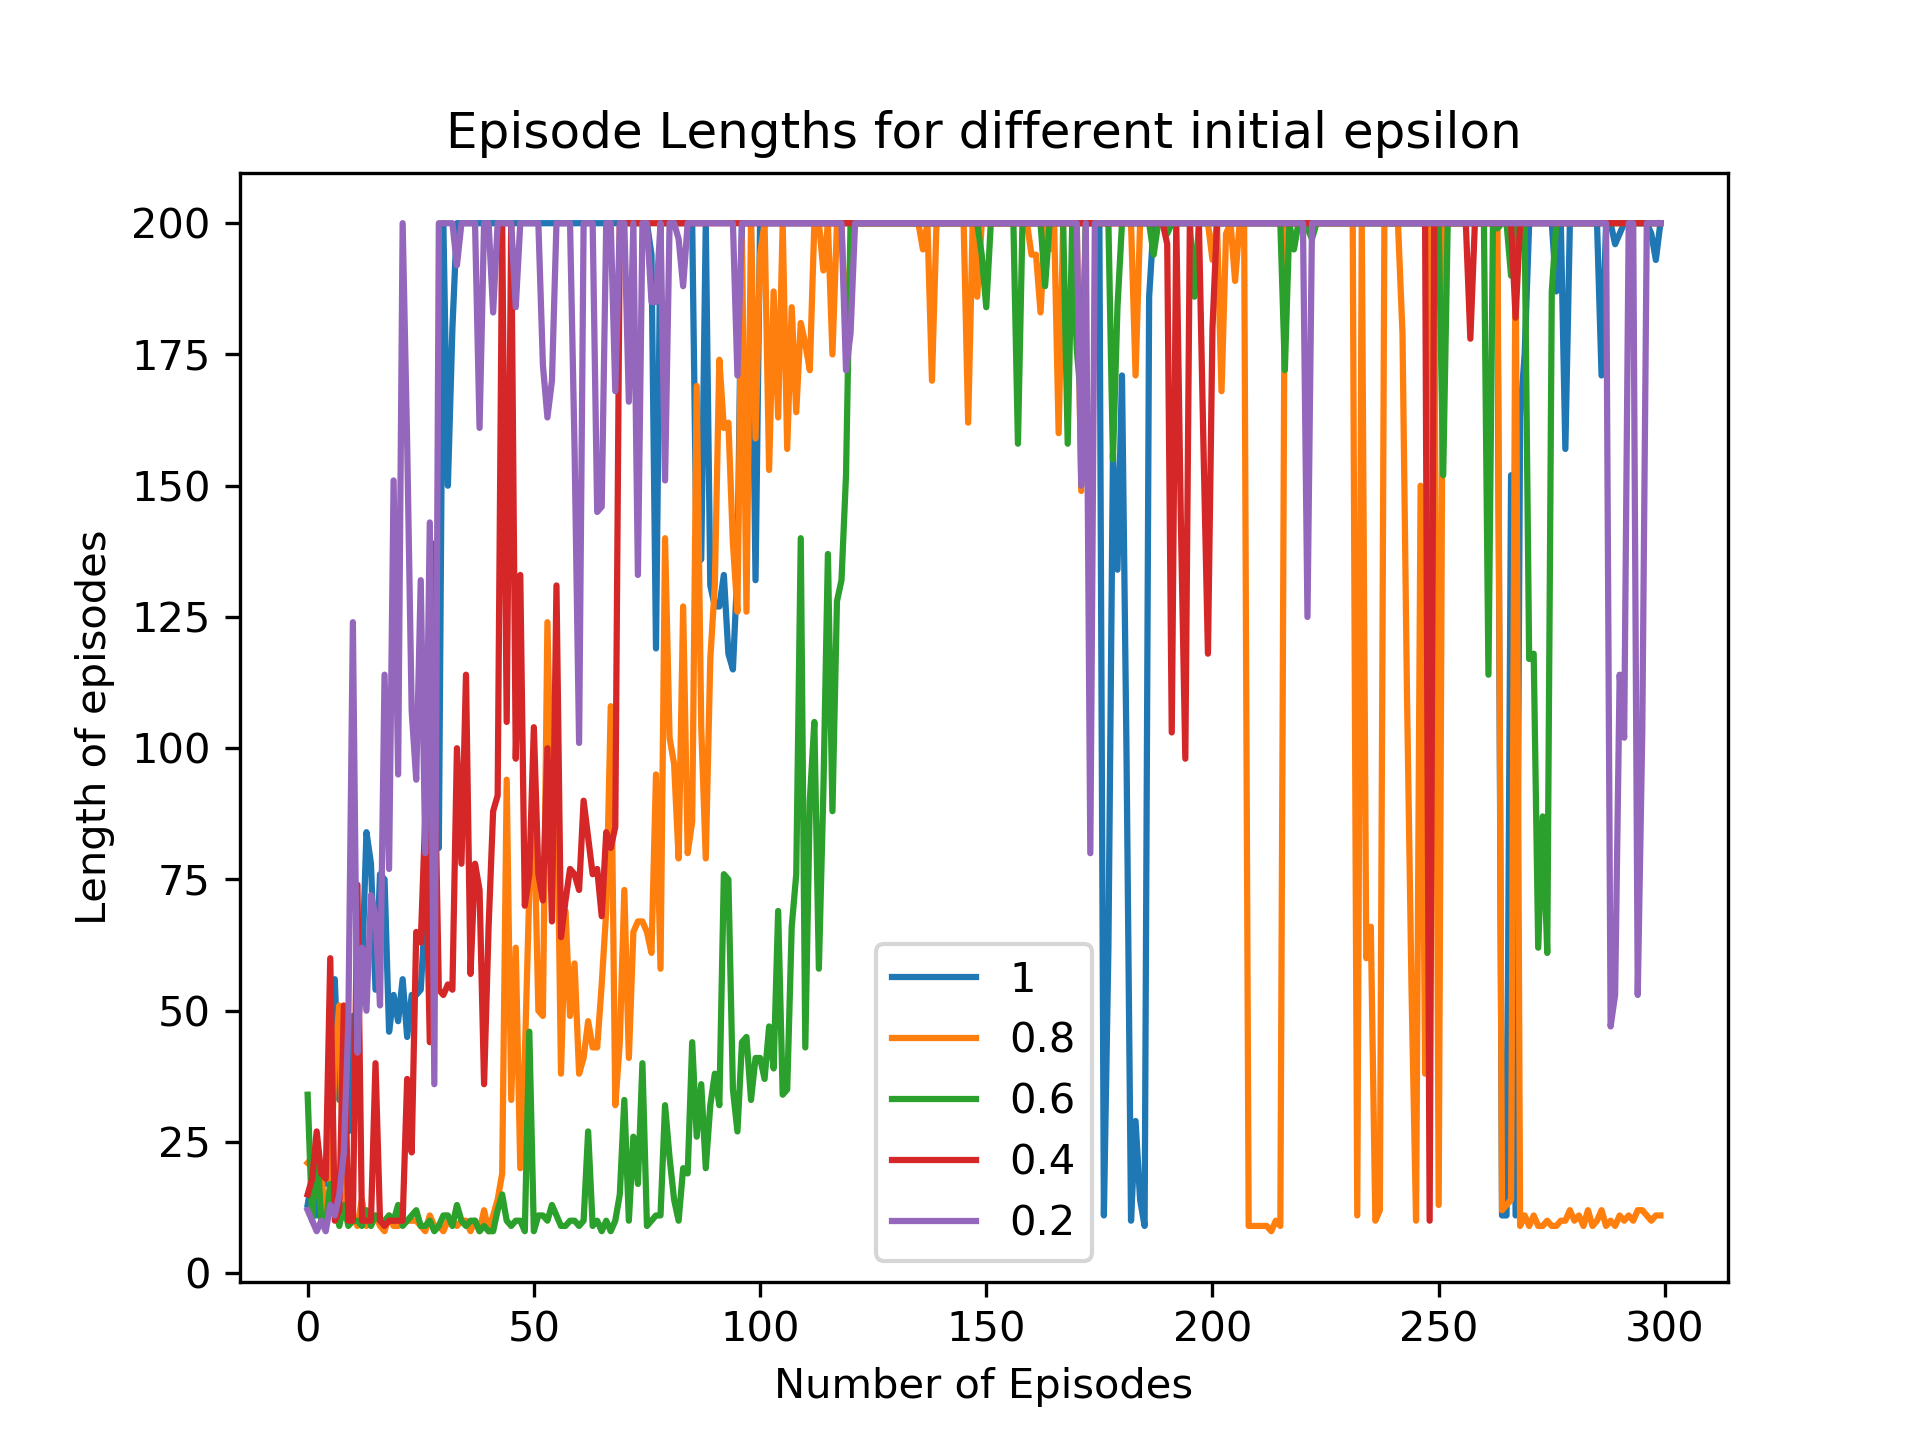
\includegraphics[width=0.4\linewidth]{./Episode_lengths_EPSILONs.png}\label{epsilon_len}}
    	\subfigure
    	{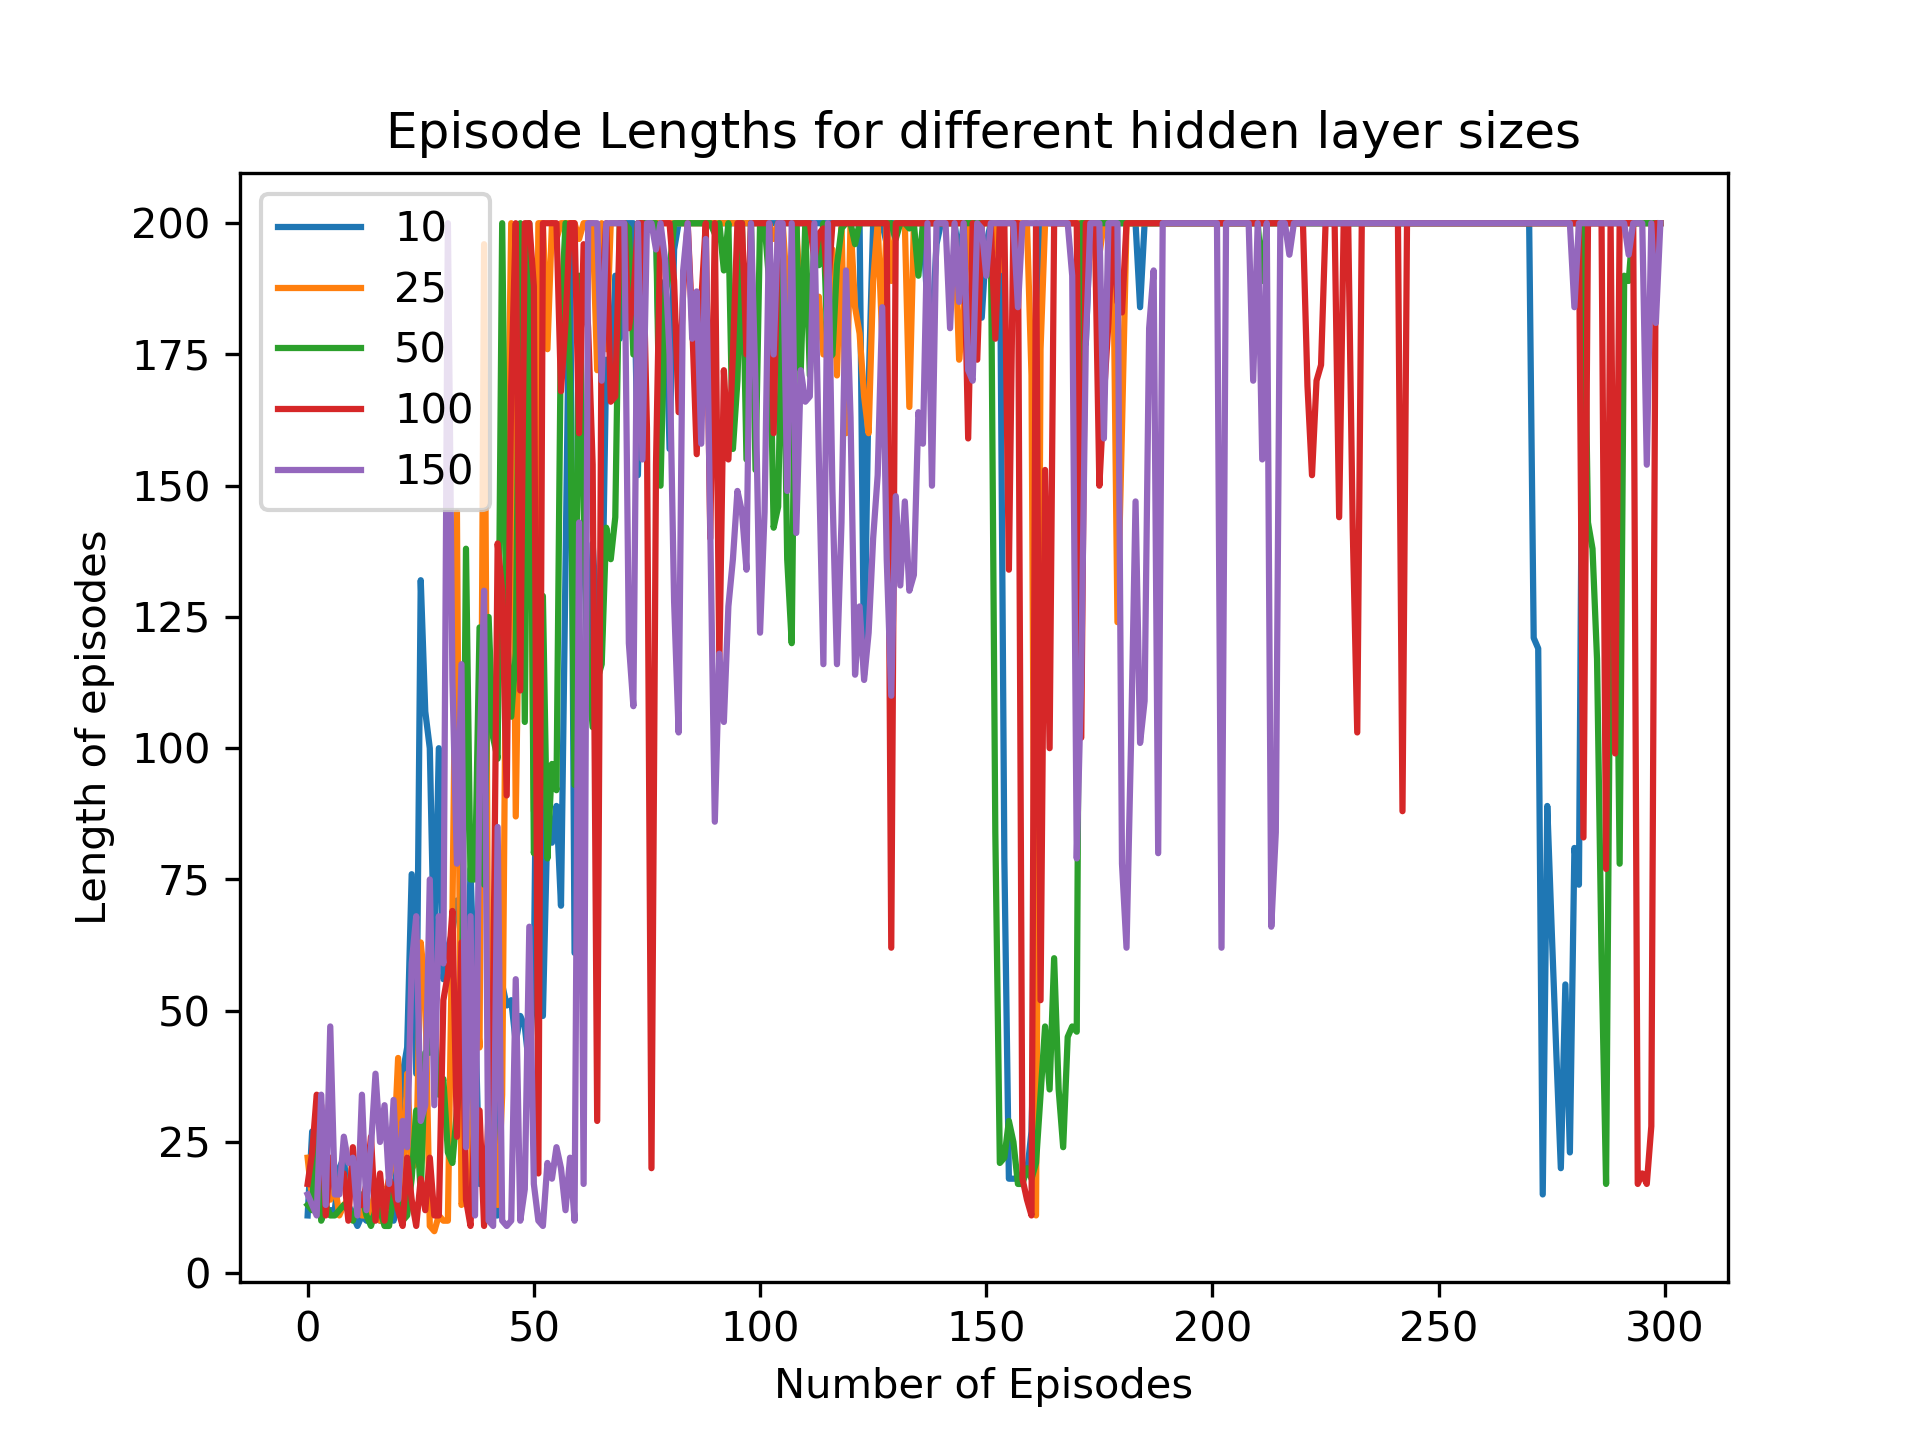
\includegraphics[width=0.4\linewidth]{./Episode_lengths_HiddenSizes.png}\label{hidden_len}}
    	\subfigure
    	{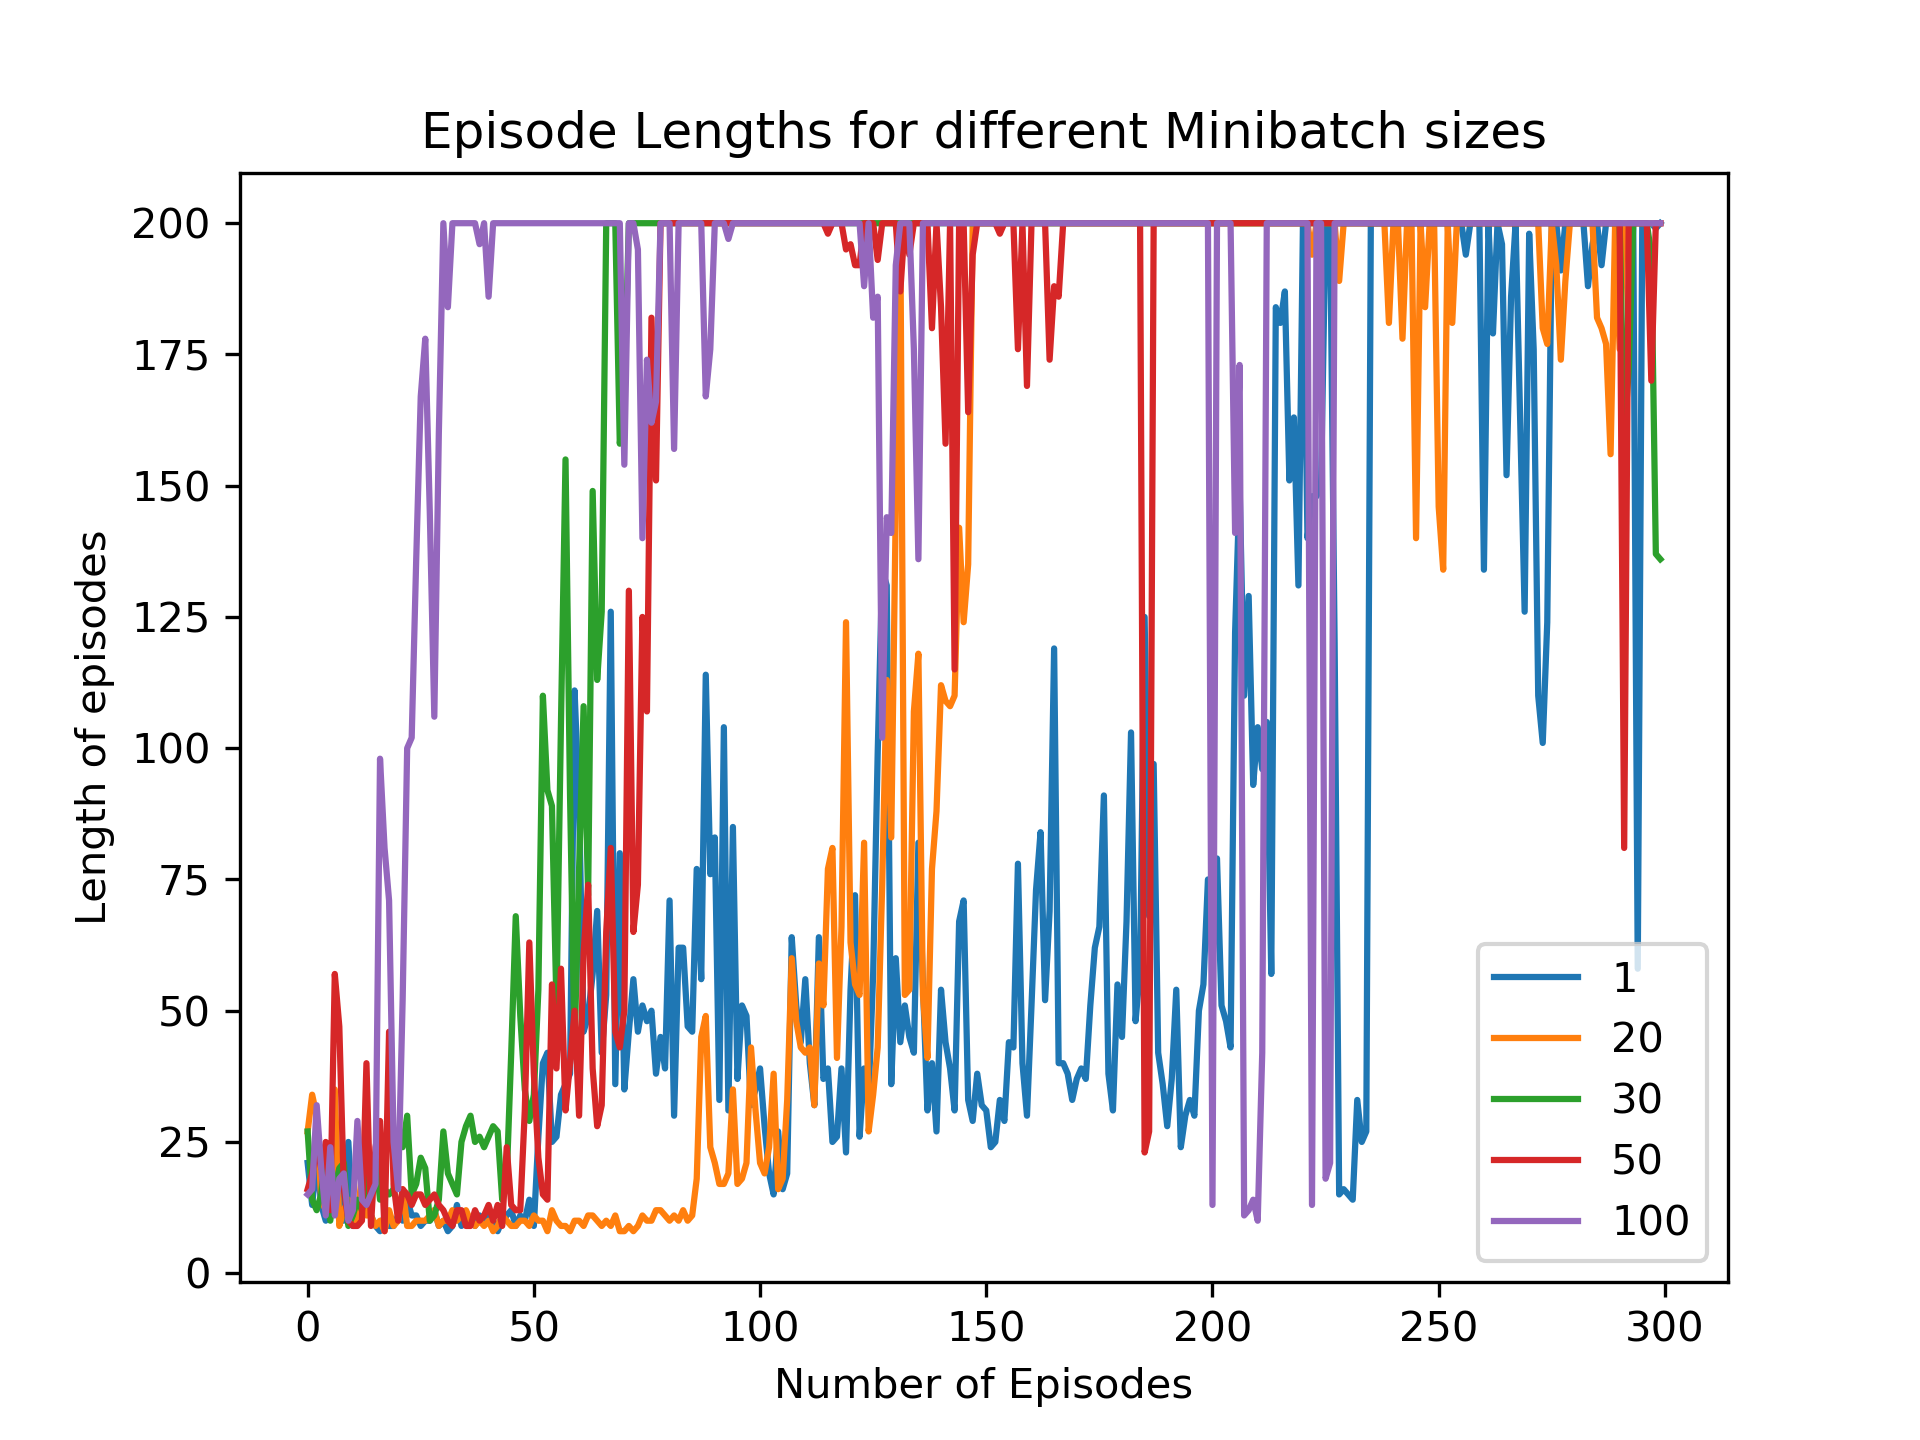
\includegraphics[width=0.4\linewidth]{./Episode_lengths_MINIBATCHs.png}\label{minibatch_len}}
    	\subfigure
    	{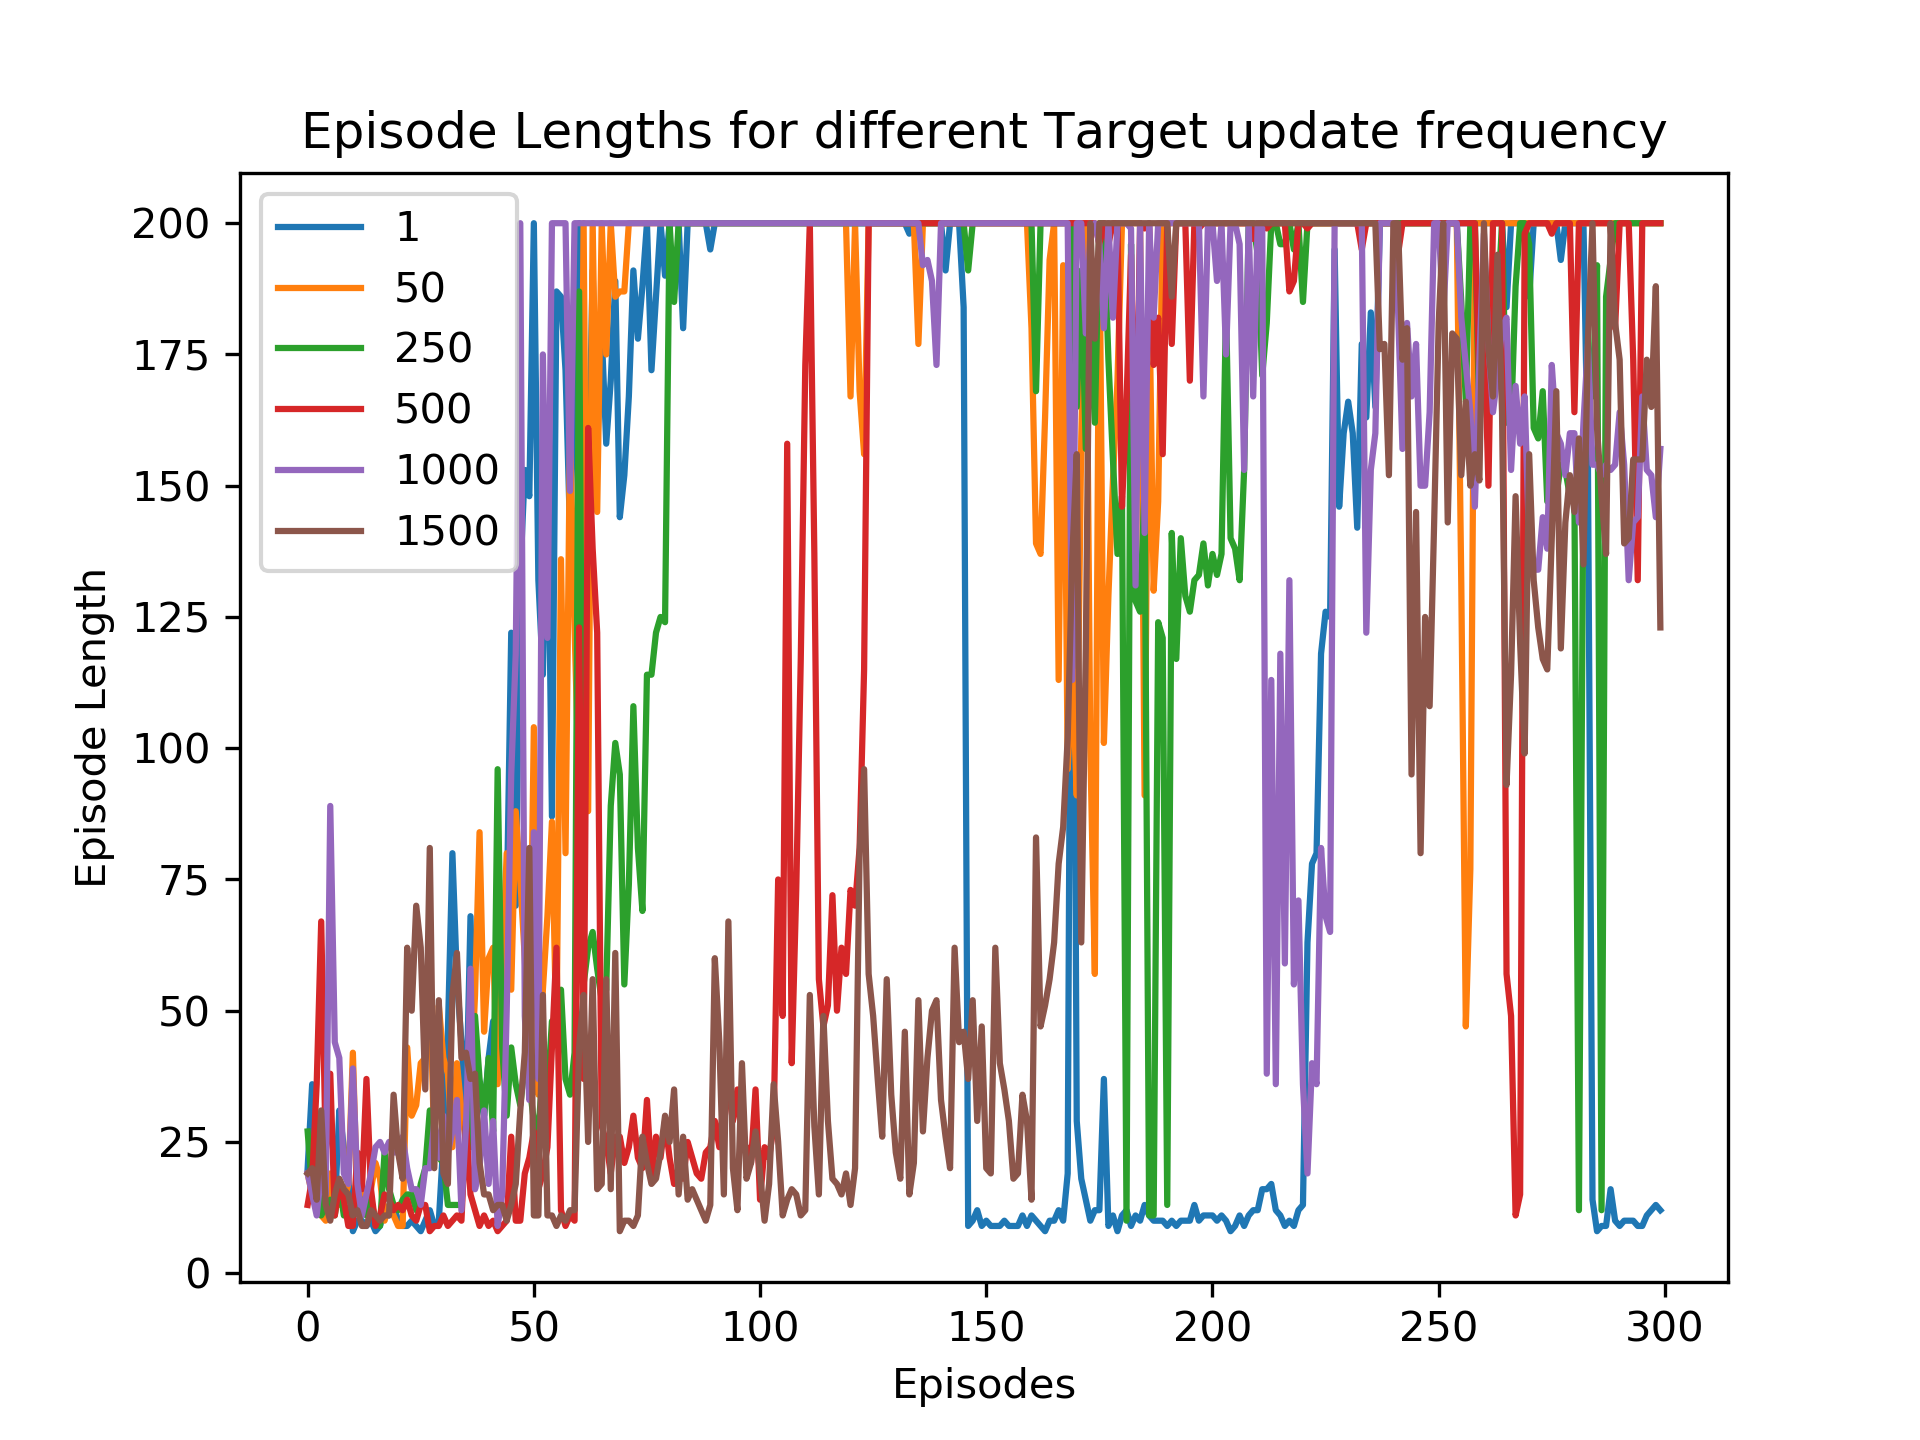
\includegraphics[width=0.4\linewidth]{./Episode_lengths_TARGETs.png}\label{target_len}}
    	\caption{Comparative Plots of episode length of different hyper parameters : Initial value of epsilon-\ref{epsilon}, Hidden layers-\ref{hidden}, size of minibatch-\ref{minibatch}, update frequency of target networks-\ref{target}}
    	\label{fig:episo_len}
    \end{figure}
    
    

  
  
\subsection{Bonus Answers-4: Observations and inferences of removal of the experience replay and/or the target network}


  
    \begin{figure}[H]
    	\centering  
    	\subfigure
    	{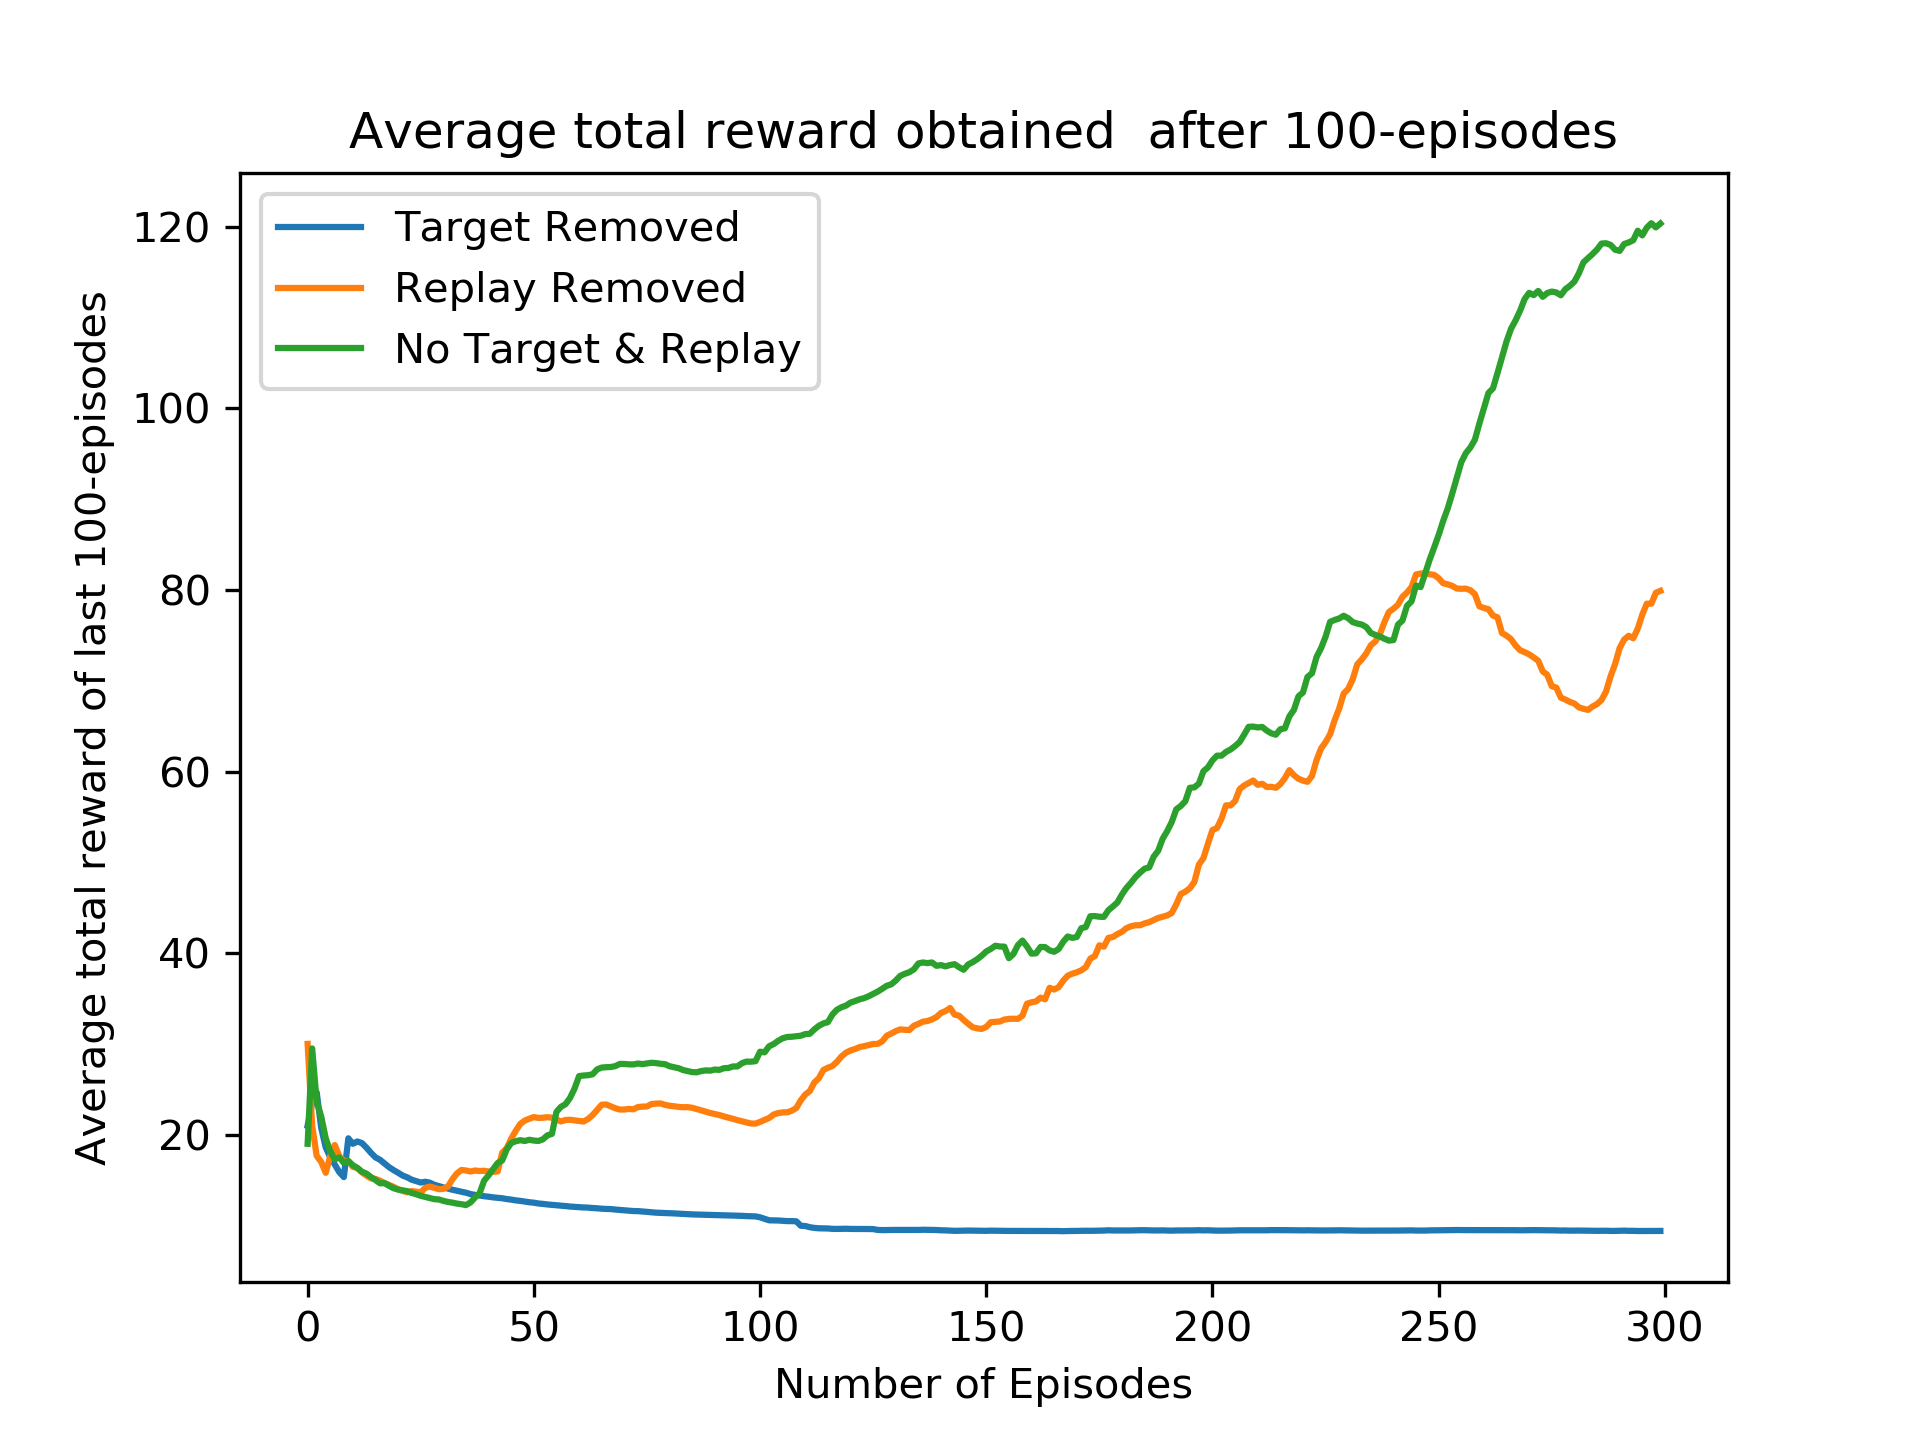
\includegraphics[width=0.4\linewidth]{./Avg_rewards_wos.png}\label{reward_wos}}
    	\subfigure
    	{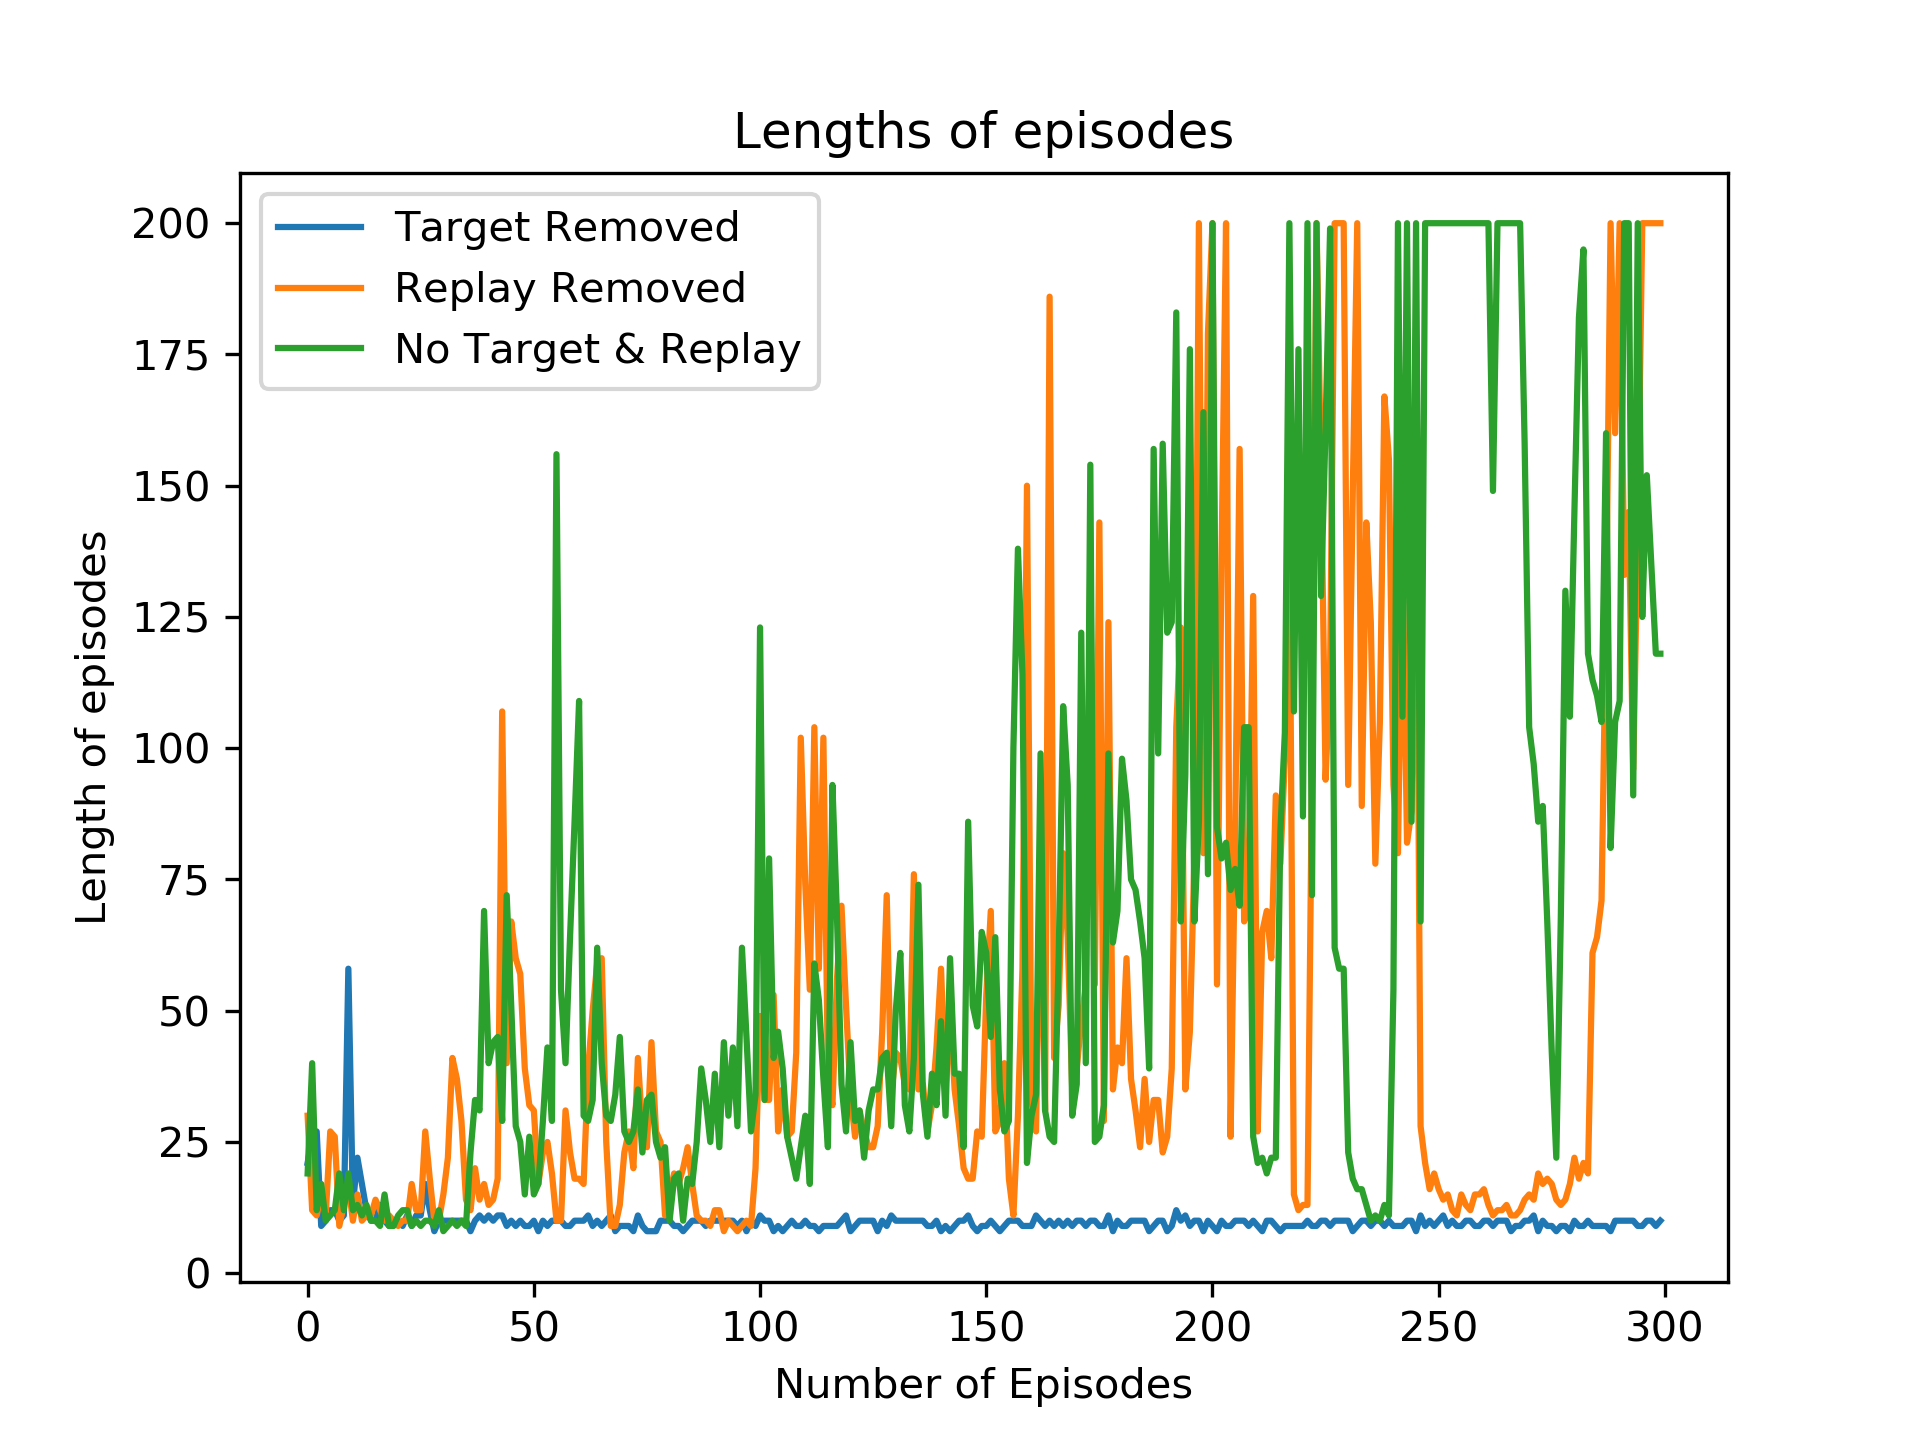
\includegraphics[width=0.4\linewidth]{./Episode_lengths_wos.png}\label{len_wos}}
    	\subfigure
    	{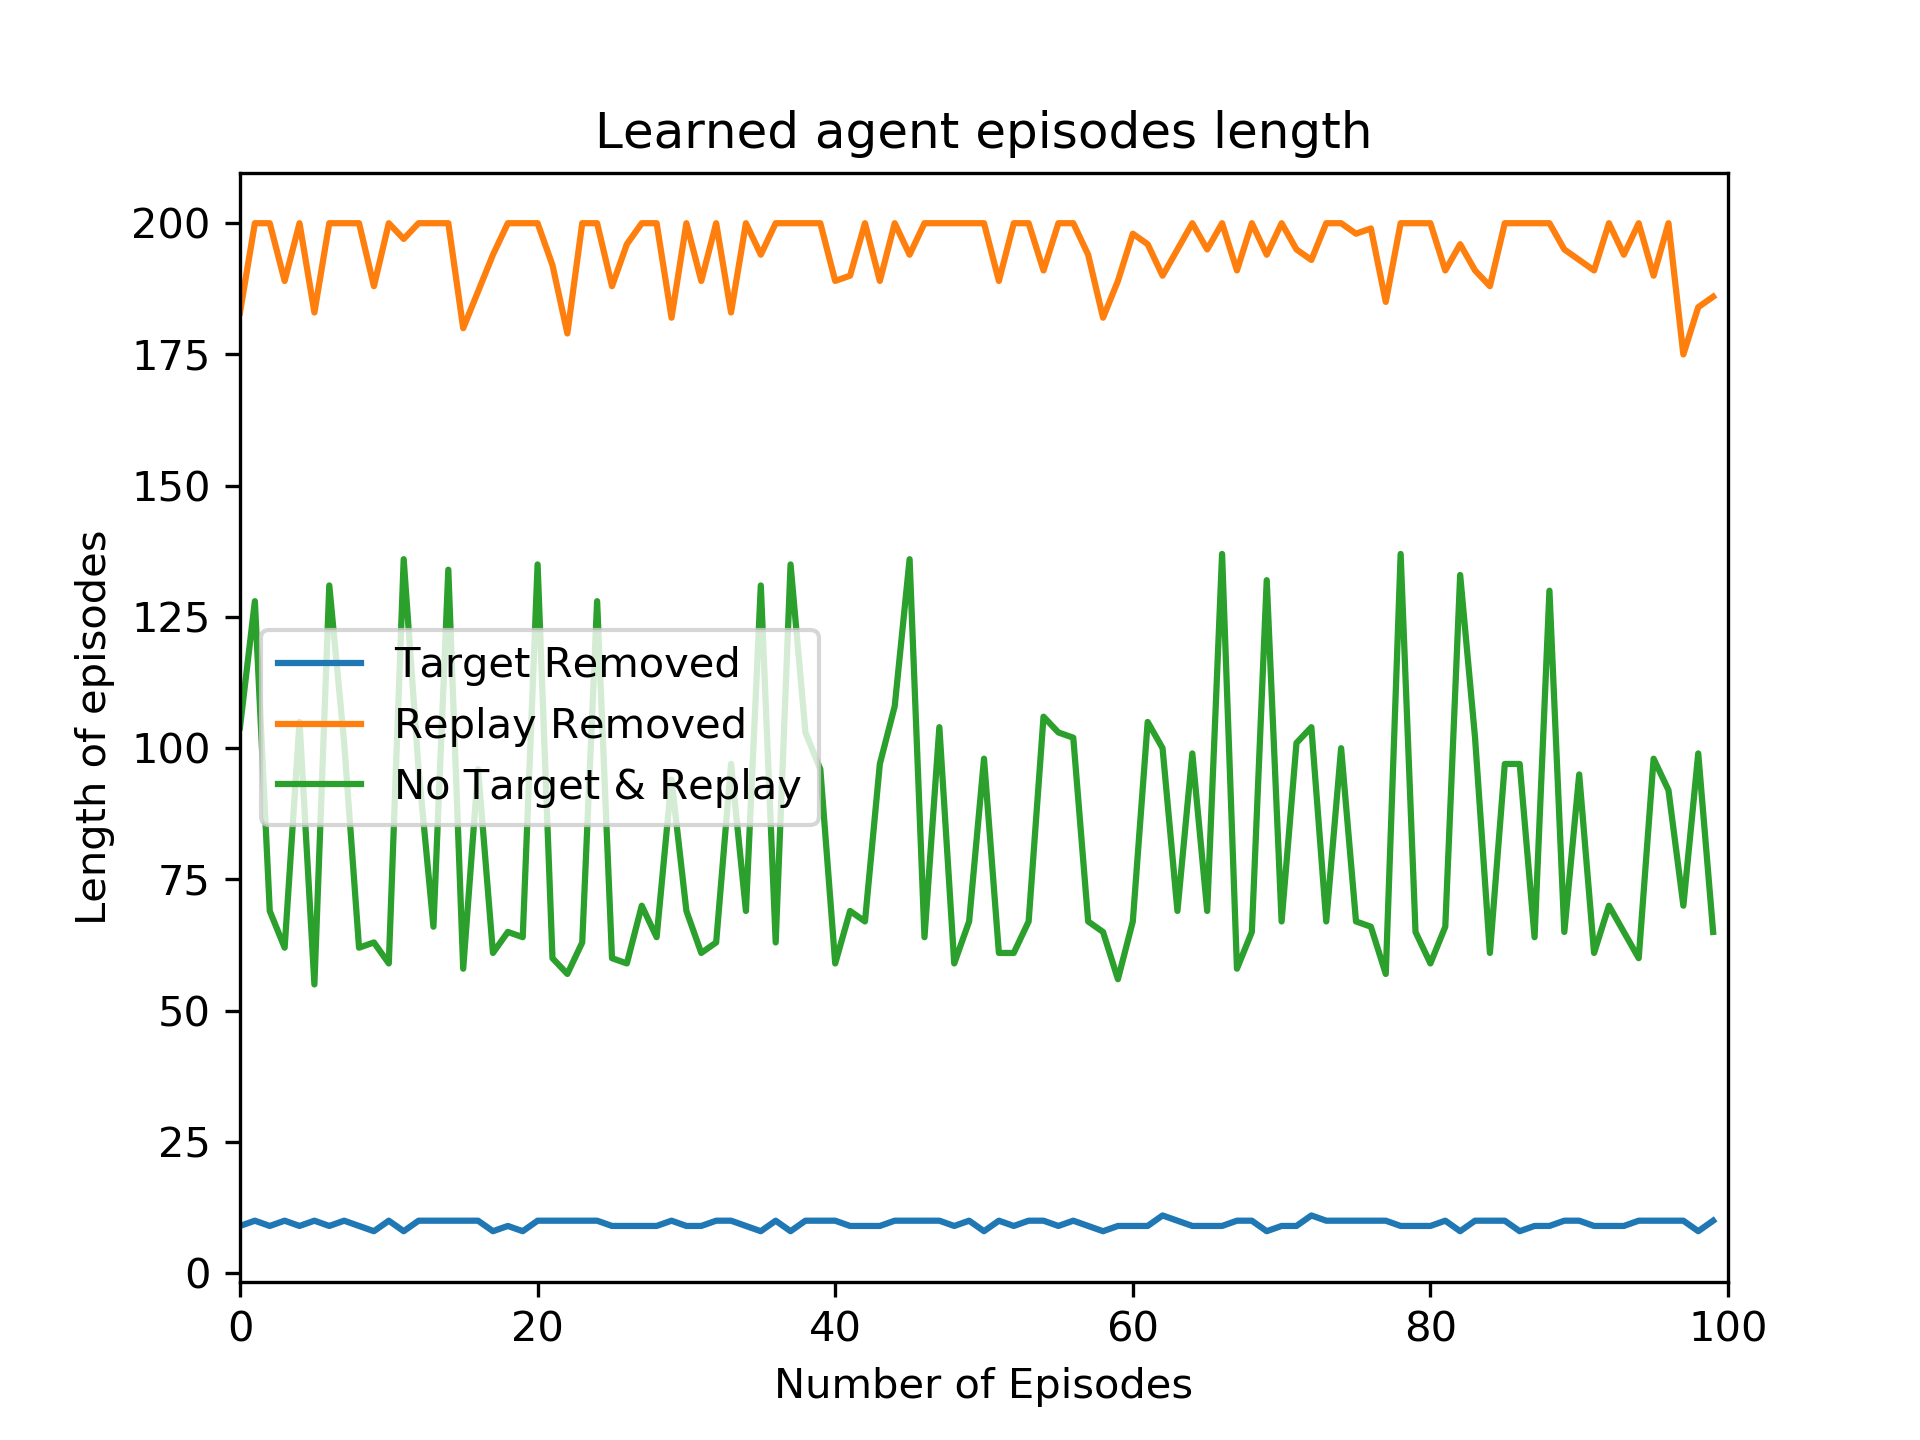
\includegraphics[width=0.4\linewidth]{./Learned_Episode_lengths_wos.png}\label{epi_wos}}
    	\caption{Plots of average reward-\ref{reward_wos}, length of episodes-\ref{epi_wos}, episode length for leaned agent-\ref{len_wos} after removing the target network, experience reply and both together. }
    	\label{fig:without}
    \end{figure}
	\newpage
	
	References:
	\\
	
	%%
	%% Following citation commands can be used in the body text:
	%% Usage of \cite is as follows:
	
	%%   \cite{key}          ==>>  [#]
	%%   \cite[chap. 2]{key} ==>>  [#, chap. 2]
	%%   \citet{key}         ==>>  Author [#]
	
	%% References with bibTeX database:
	\bibliographystyle{ieeetr}
	\bibliography{biblio.bib}					
	%% Authors are advised to submit their bibtex database files. They are
	%% requested to list a bibtex style file in the manuscript if they do
	%% not want to use model1-num-names.bst.
	
	%% References without bibTeX database:
	
	% \begin{thebibliography}{00}
	
	%% \bibitem must have the following form:
	%%   \bibitem{key}...
	%%
	
	% \bibitem{}
	
	% \end{thebibliography}


\end{document}